\chapter{Hadronic Resonance Identification}
\label{sec:jets}

In this chapter, we describe the reconstruction and identification of heavy ($\gtrsim 100$ GeV) resonances that decay to two or more quarks.
Within the Standard Model, the only such resonances are the massive vector bosons ($W,Z\rightarrow q\bar{q}'$), the Higgs boson (typically $H\rightarrow b\bar{b}$), and the top quark ($t\rightarrow bW(\rightarrow q\bar{q}')$).
The focus of this chapter is on the cases in which the resonance is boosted and the decay products merge, such that they cannot be identified as 2 or 3 distinct AK4 jets.
In preparation for Chapter~\ref{sec:mt}, we will take the top quark as a concrete example.
The studies presented here can, and in some cases have been, applied to other heavy resonances, both within and beyond the Standard Model.

\section{Reconstruction}
\label{sec:jets:reco}

The need for a dedicated boosted top jet reconstruction arises from the momentum-dependence of the angular separation between the quarks from a heavy resonance decay~\cite{tasijets}:
\begin{equation}
    \Delta R \sim \frac{2M}{\pt}
    \label{eq:jets:dr}
\end{equation}
where $M$ is the resonance mass and $\pt$ is the resonance transverse momentum.
If $\pt\gtrsim300$ GeV and $M = m_t$, then $\Delta R = 1.2$.
At this separation, three AK4 jets will begin to overlap, reducing the efficiency of reconstructing each of the daughter quarks separately.
This is verified by checking the distribution of the \emph{decay radius} in top quark simulation.
Here, we define decay radius as: 
\begin{equation}
    \max\Delta R_{qq} \equiv \displaystyle\max_{0\leq i < j \leq 2} \{\Delta R(q_i,q_j)\} \text{, where } t\rightarrow q_0q_1q_2
\end{equation}
Using a broad spectrum of generated top quark $\pt$, Figure~\ref{fig:jets:dr} shows the dependence of the decay radius on the top quark $\pt$.

The analysis described in Chapter~\ref{sec:mt} targets top jets with $\pt>250$ GeV.
Figure~\ref{fig:jets:dr} and Equation~\ref{eq:jets:dr} both indicate that at this momentum, a three-jet reconstruction is not optimal.
In particular, Figure~\ref{fig:jets:dr} shows that for $\pt\approx 250$ GeV, it is equally likely that a top quark's decay products will fall within a single $R=1.5$ jet or that they will be resolvable as three separate jets. 
However, past this threshold momentum, the large-radius jet becomes the preferred reconstruction option.
This motivates the use of $R=1.5$ jets to reconstruct hadronic top quarks with $\pt>250$ GeV. 

\begin{figure}[]
    \begin{center}
        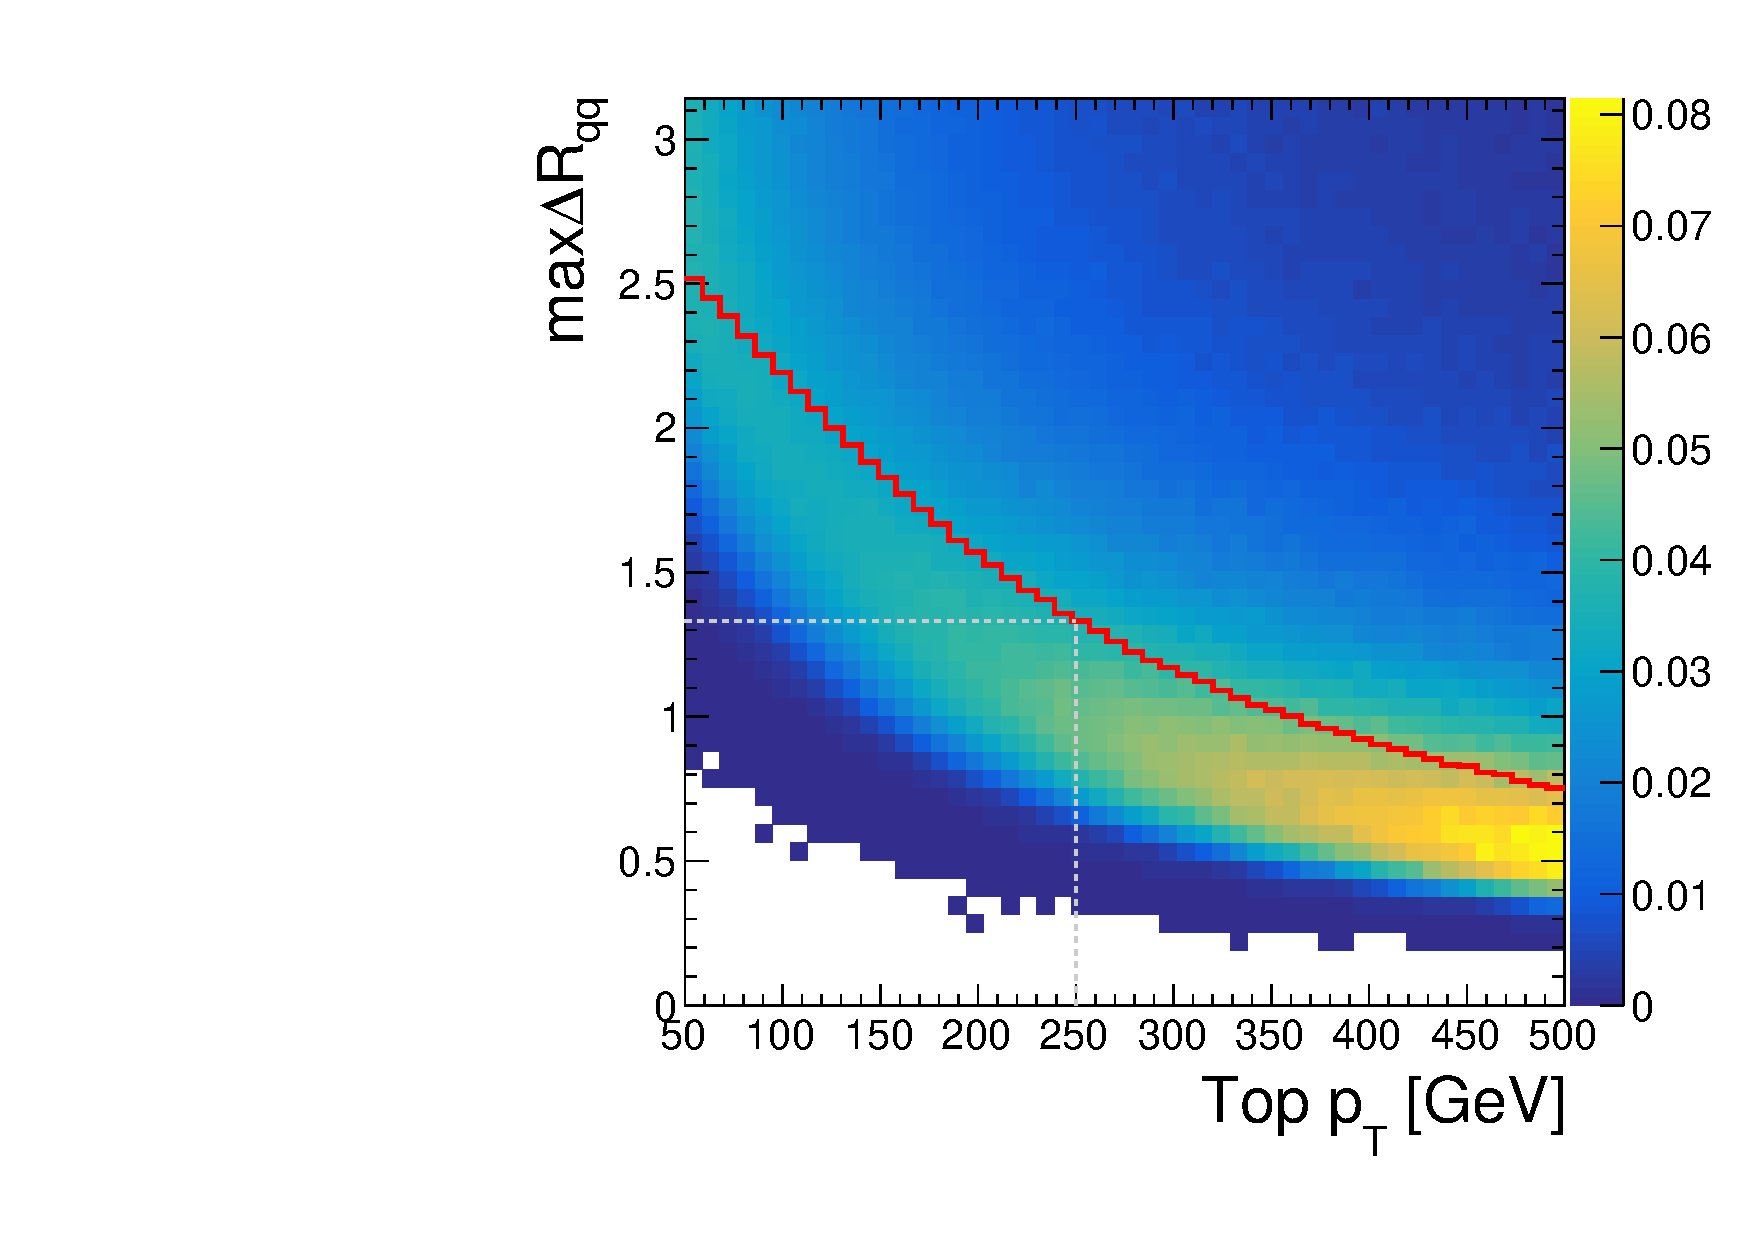
\includegraphics[width=0.5\textwidth]{figures/toptagging/gen/ptdr.pdf}
        \caption{Distribution of top quark momenta versus decay radii in a simulated top quark pair sample.
                 The events are weighted such that the inclusive momentum distribution is uniform. 
                 The $z$-axis units are arbitrary, but proportional to the distribution of jets. 
                 The solid red line marks the 50\% quantile of jets at each value of $\pt$. }
        \label{fig:jets:dr}
    \end{center}
\end{figure}

There are two tunable parameters in jet reconstruction.
We have specified the jet radius, but we must also choose the jet algorithm.
The anti-$k_\mathrm{T}$ algorithm tends to pick circular jets, whereas the Cambridge-Aachen (CA) algorithm results in more geometric shapes (Figure~\ref{fig:jets:algos}).
As the top jets we seek to reconstruct are the sum of three light quark jets, we do not necessarily expect the $R=1.5$ jet to be circular.
Figure~\ref{fig:jets:caak} compares the jet mass distribution for top and light quark/gluon (LQG) jets, where the jets are clustered using both algorithms.
CA produces a top jet mass distribution with a narrower peak closer to $m_t$ than anti-\kt, which is why we choose the CA algorithm. 
Hereafter, we will refer to Cambridge-Aachen $R=1.5$ jets as CA15 jets. 

\begin{figure}[]
    \begin{center}
        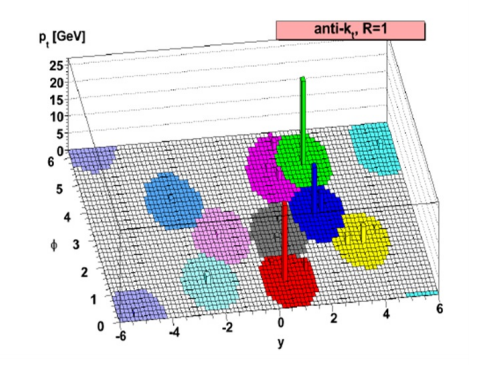
\includegraphics[width=0.35\textwidth]{figures/toptagging/gen/ak.png}
        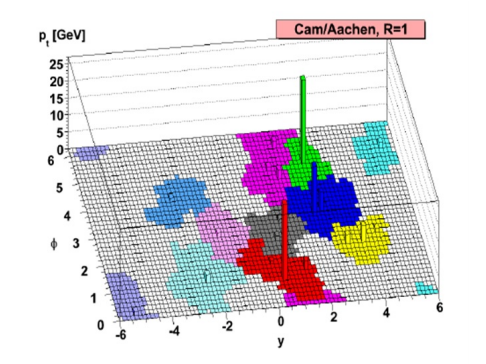
\includegraphics[width=0.35\textwidth]{figures/toptagging/gen/ca.png}
        \caption{Jets clustered using the anti-$k_\mathrm{T}$ (left) and CA (right) algorithms.
                 Shown is the $y$-$\phi$ plane of a hypothetical calorimeter, unrolled onto a flat surface.
                 The height of each cell represents the \pt~of the particle. 
                 The anti-\kt~jets tend to be more circular when compared to the CA jets.
                 Figures are adapted from~\cite{antikt}.}
        \label{fig:jets:algos}
    \end{center}
\end{figure}

\begin{figure}[]
    \begin{center}
        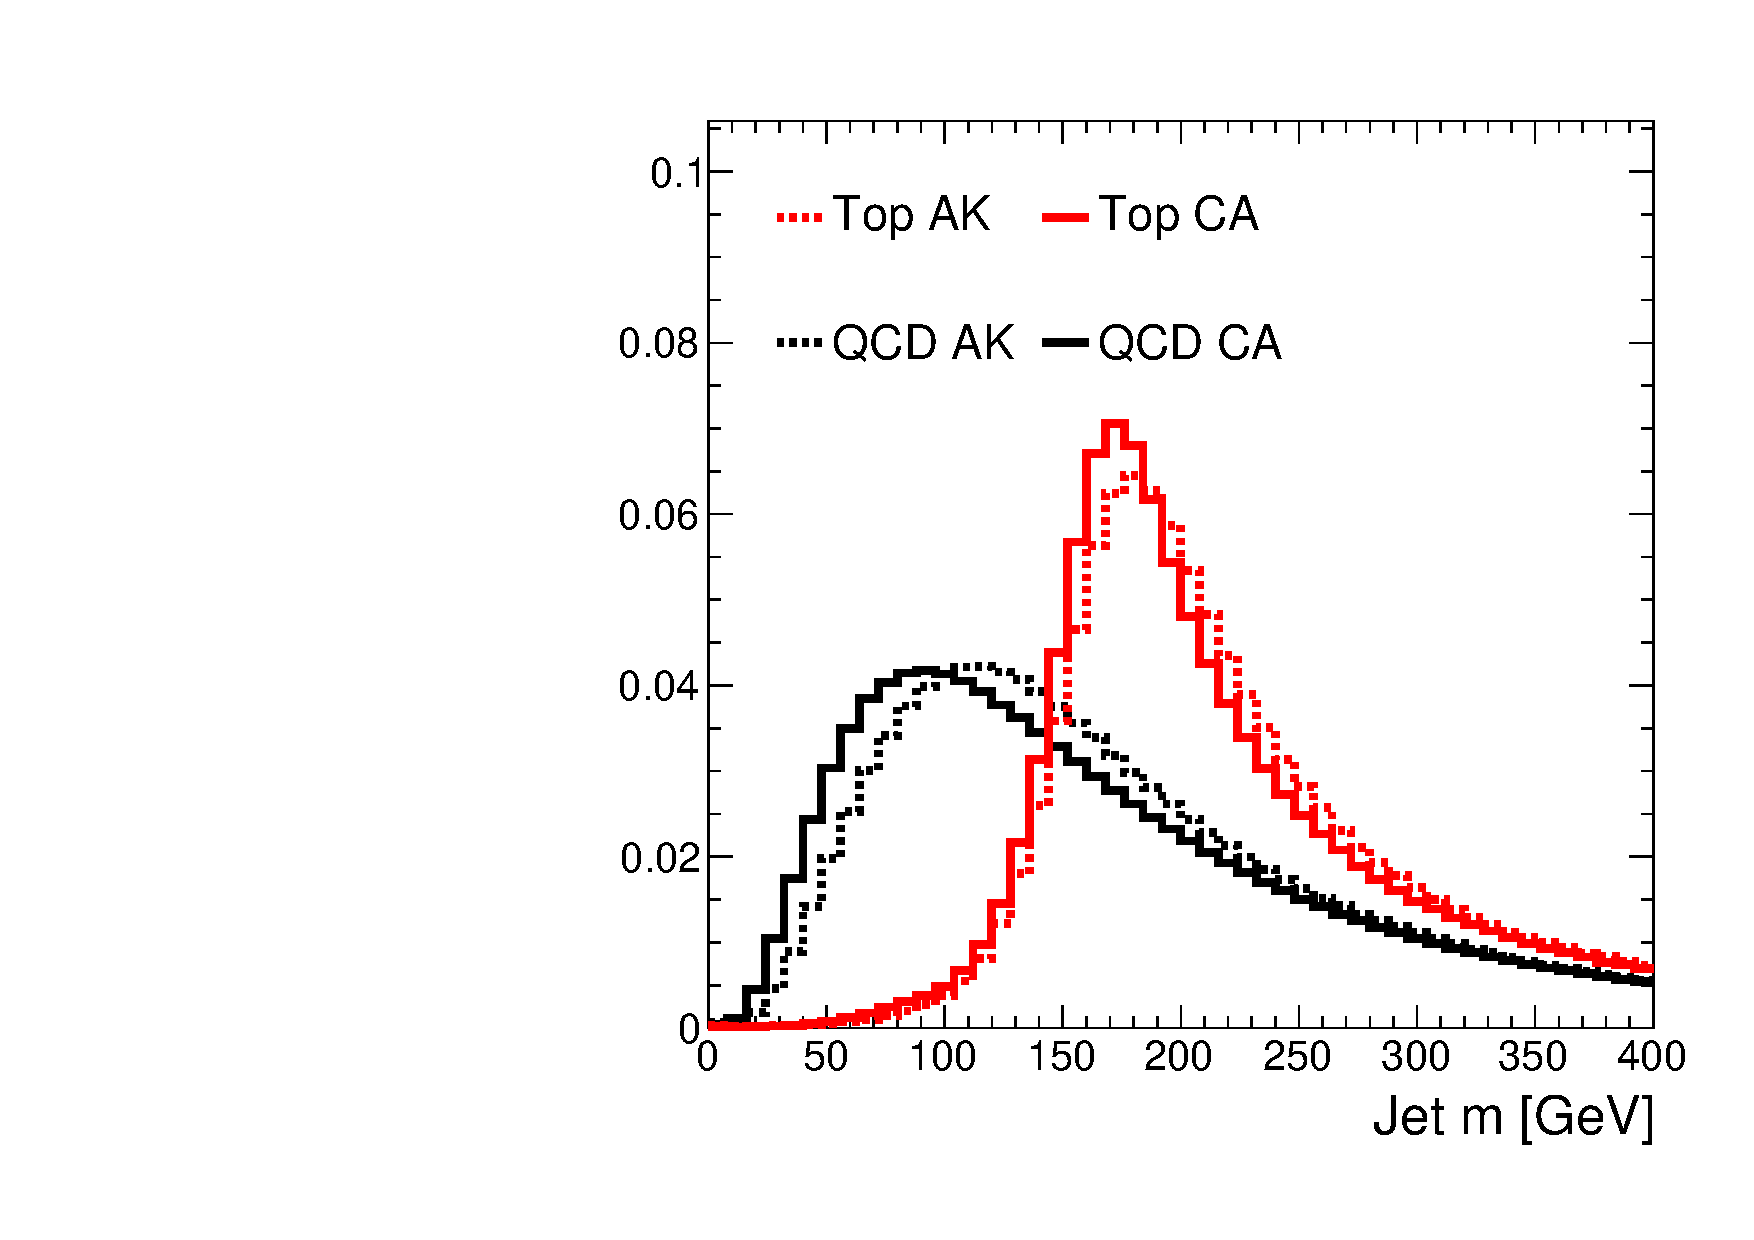
\includegraphics[width=0.5\textwidth]{figures/toptagging/gen/clf_M.pdf}
        \caption{Mass distribution for jets clustered using the anti-$k_\mathrm{T}$ (dashed) and CA (solid) algorithms.
                 QCD refers to jets originating in QCD multijet events, i.e.~from the hadronization of light quarks or gluons.
                 The CA top peak is slightly sharper than the anti-\kt~peak, is closer to $m_t$, and the QCD background is slightly lower near the peak.
                 }
        \label{fig:jets:caak}
    \end{center}
\end{figure}

The distance parameter of $R=1.5$ corresponds approximately to a maximal azimuthal angle separation of $\nicefrac{\pi}{2}$, which can cover half of the detector's fiducial volume.
As the jet is so large, particles from pile-up interactions may be clustered into a jet from the primary vertex.
Fundamental quantities (like top quark momentum) are uncorrelated with \NPV, but reconstructed quantities acquire such a dependence due to the extra radiation.
These additional particles bias the energy scale of the jet, as well as other observables.
To mitigate these effects, we scale the particles' 4-momenta by their corresponding PUPPI scores (described in Chapter~\ref{sec:cms}) prior to clustering the jet.
Jets clustered without PUPPI weighting have a jet mass and $\tau_{32}^\mathrm{SD}$ distributions (Figure~\ref{fig:jets:puppi}) in which both the mean and variance are dependent on \NPV.
Subjecting particles to PUPPI prior to clustering strongly reduces this dependence.

\begin{figure}[]
    \begin{center}
        \begin{subfigure}[t]{0.35\textwidth}
            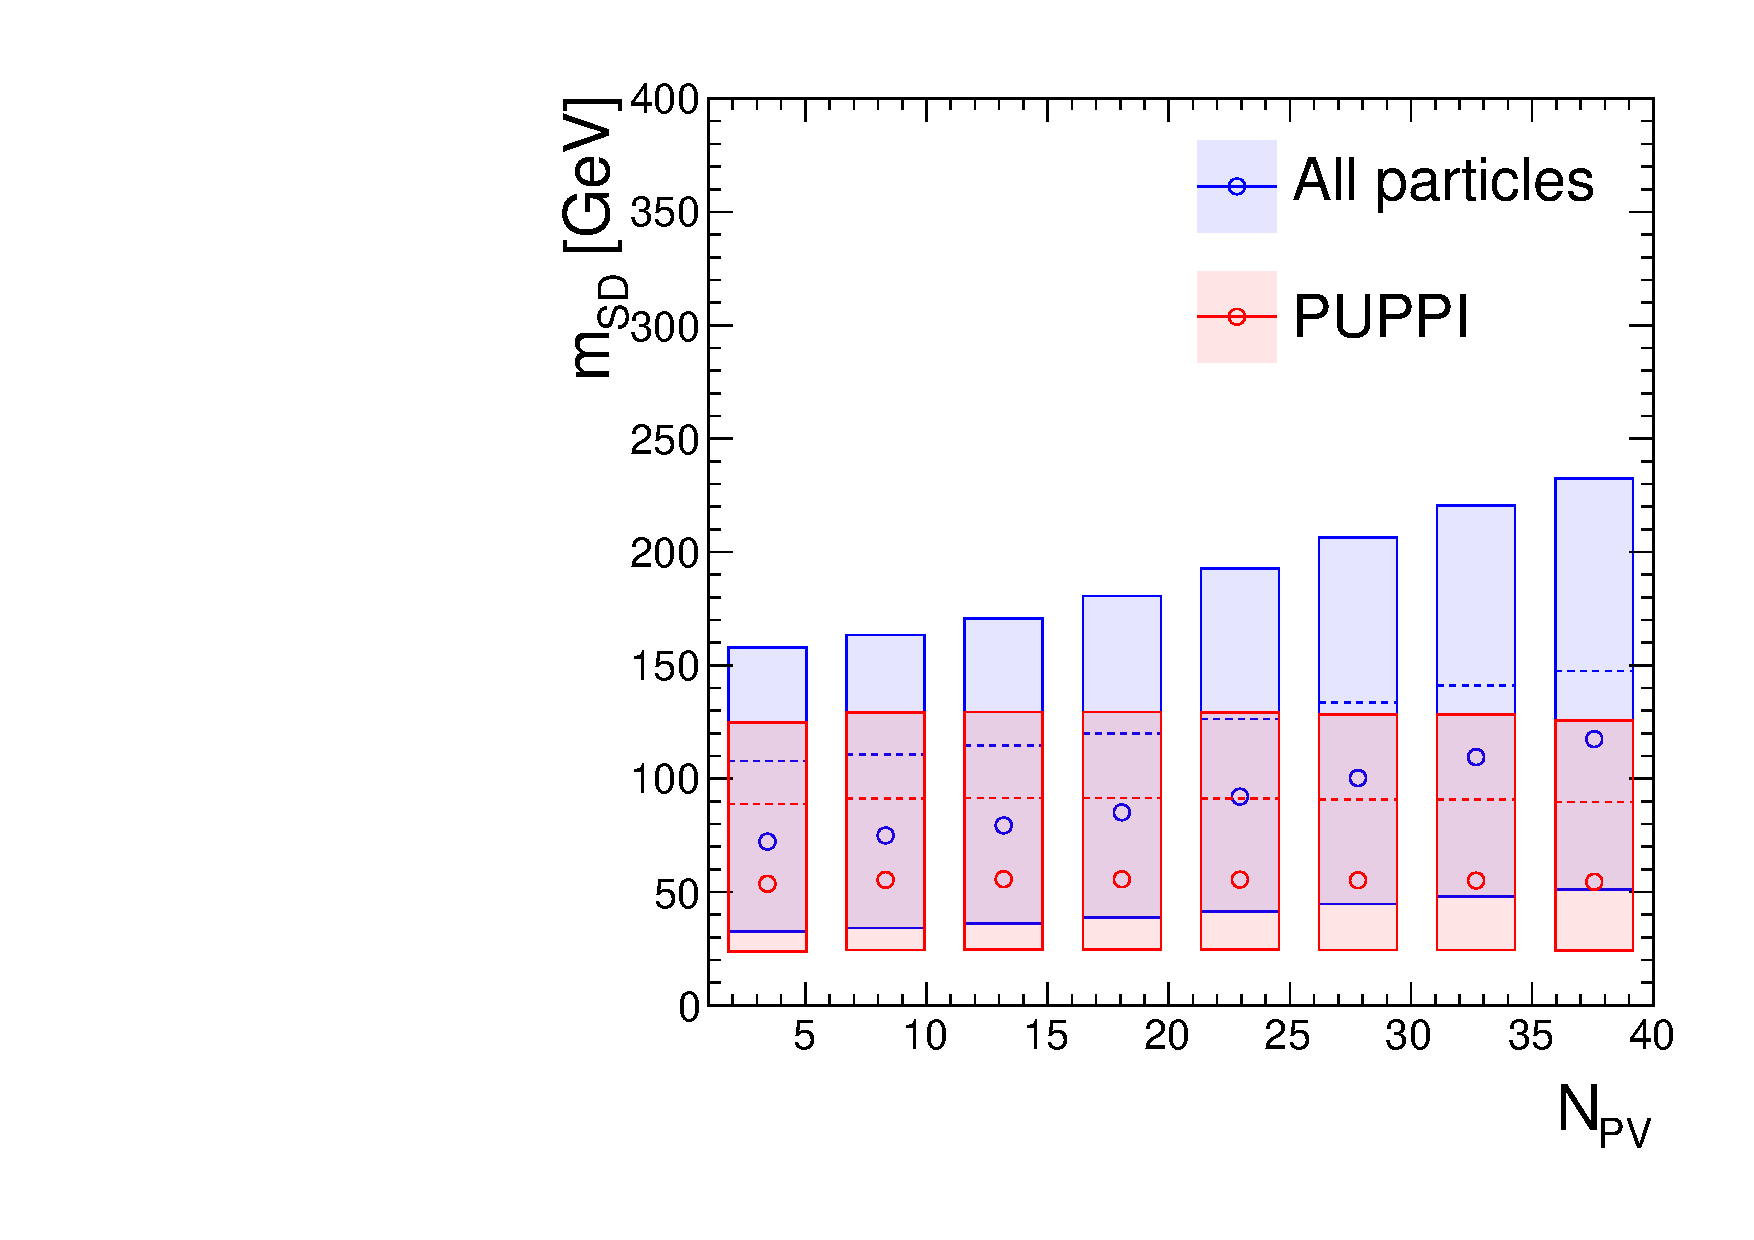
\includegraphics[width=\textwidth]{figures/toptagging/gen/npv_clf_MSD_QCD.pdf}
            \caption{Jet mass, LQG}
        \end{subfigure}
        \begin{subfigure}[t]{0.35\textwidth}
            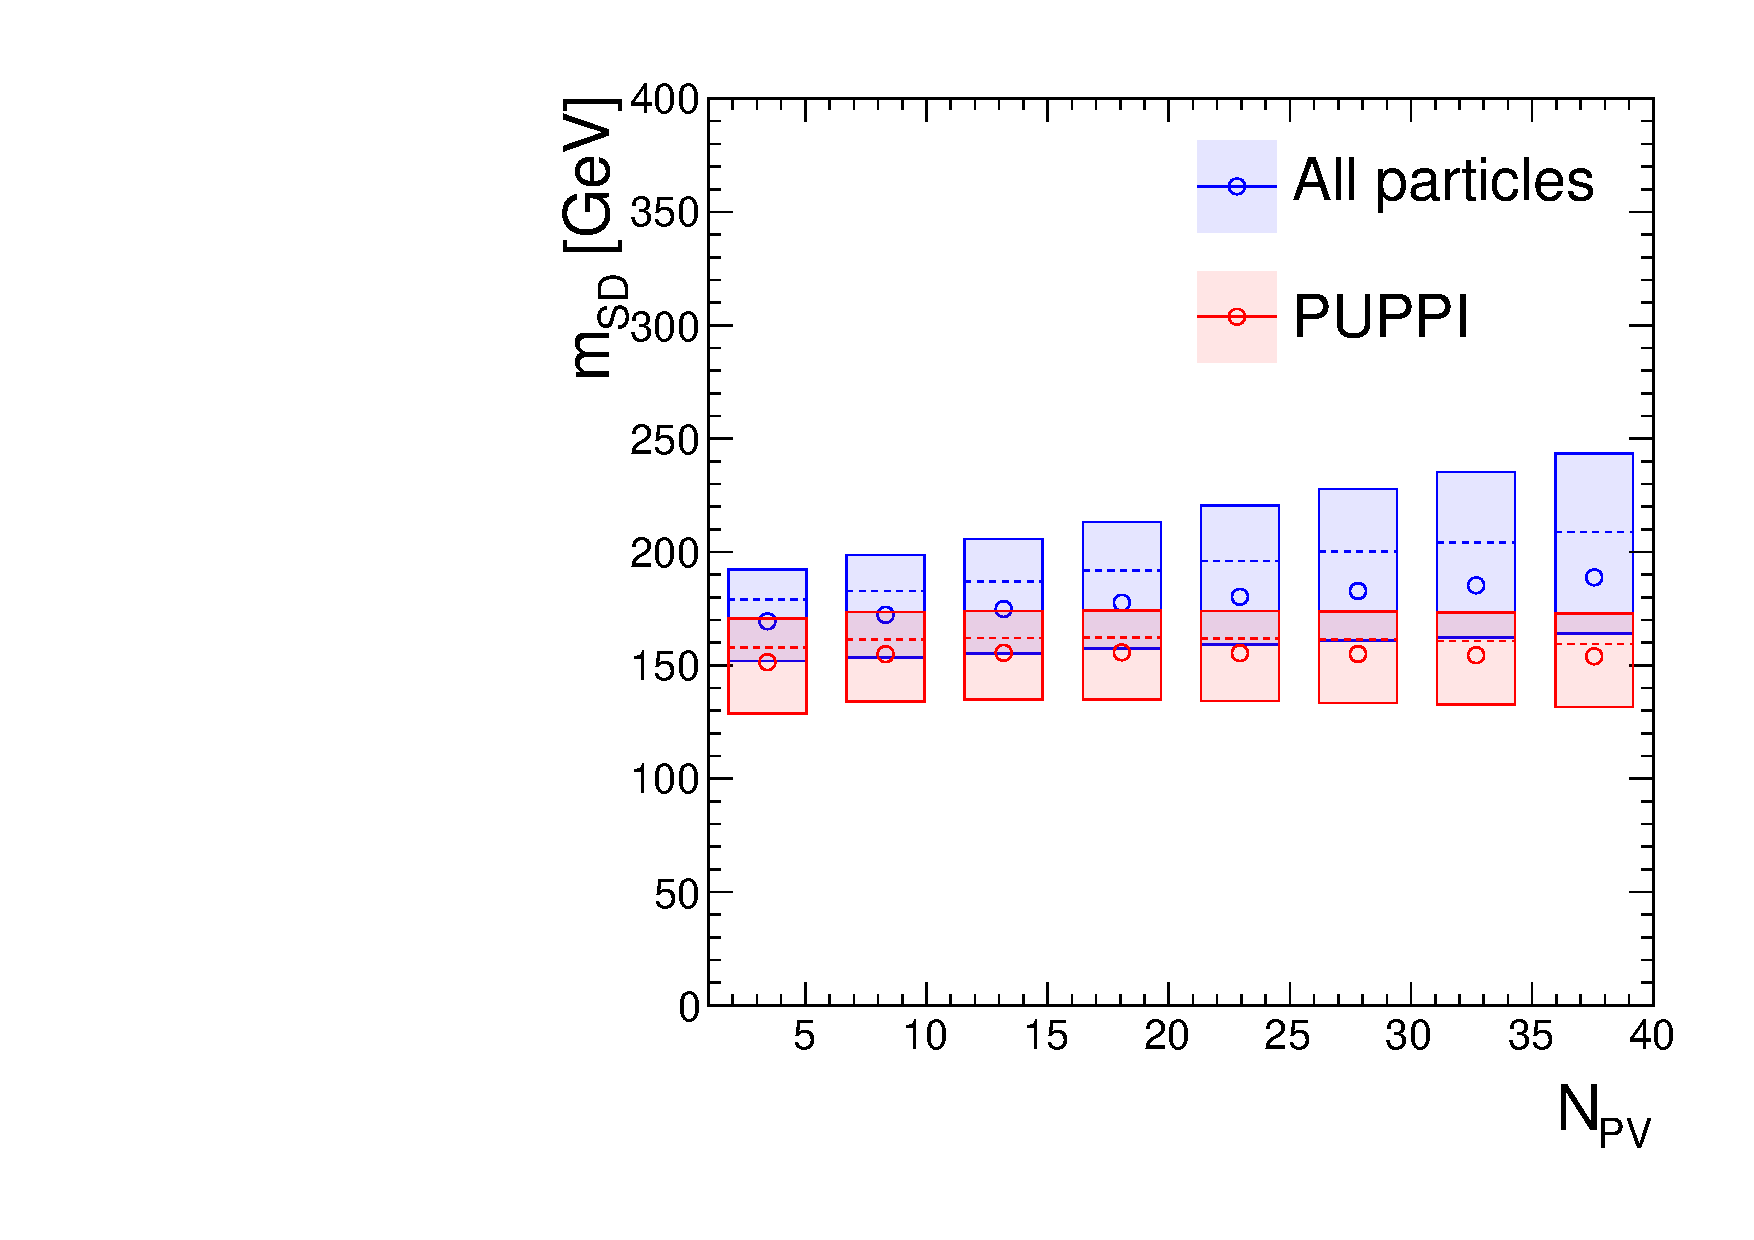
\includegraphics[width=\textwidth]{figures/toptagging/gen/npv_clf_MSD_ZpTT_lo.pdf}
            \caption{Jet mass, Top}
        \end{subfigure}
        \begin{subfigure}[t]{0.35\textwidth}
            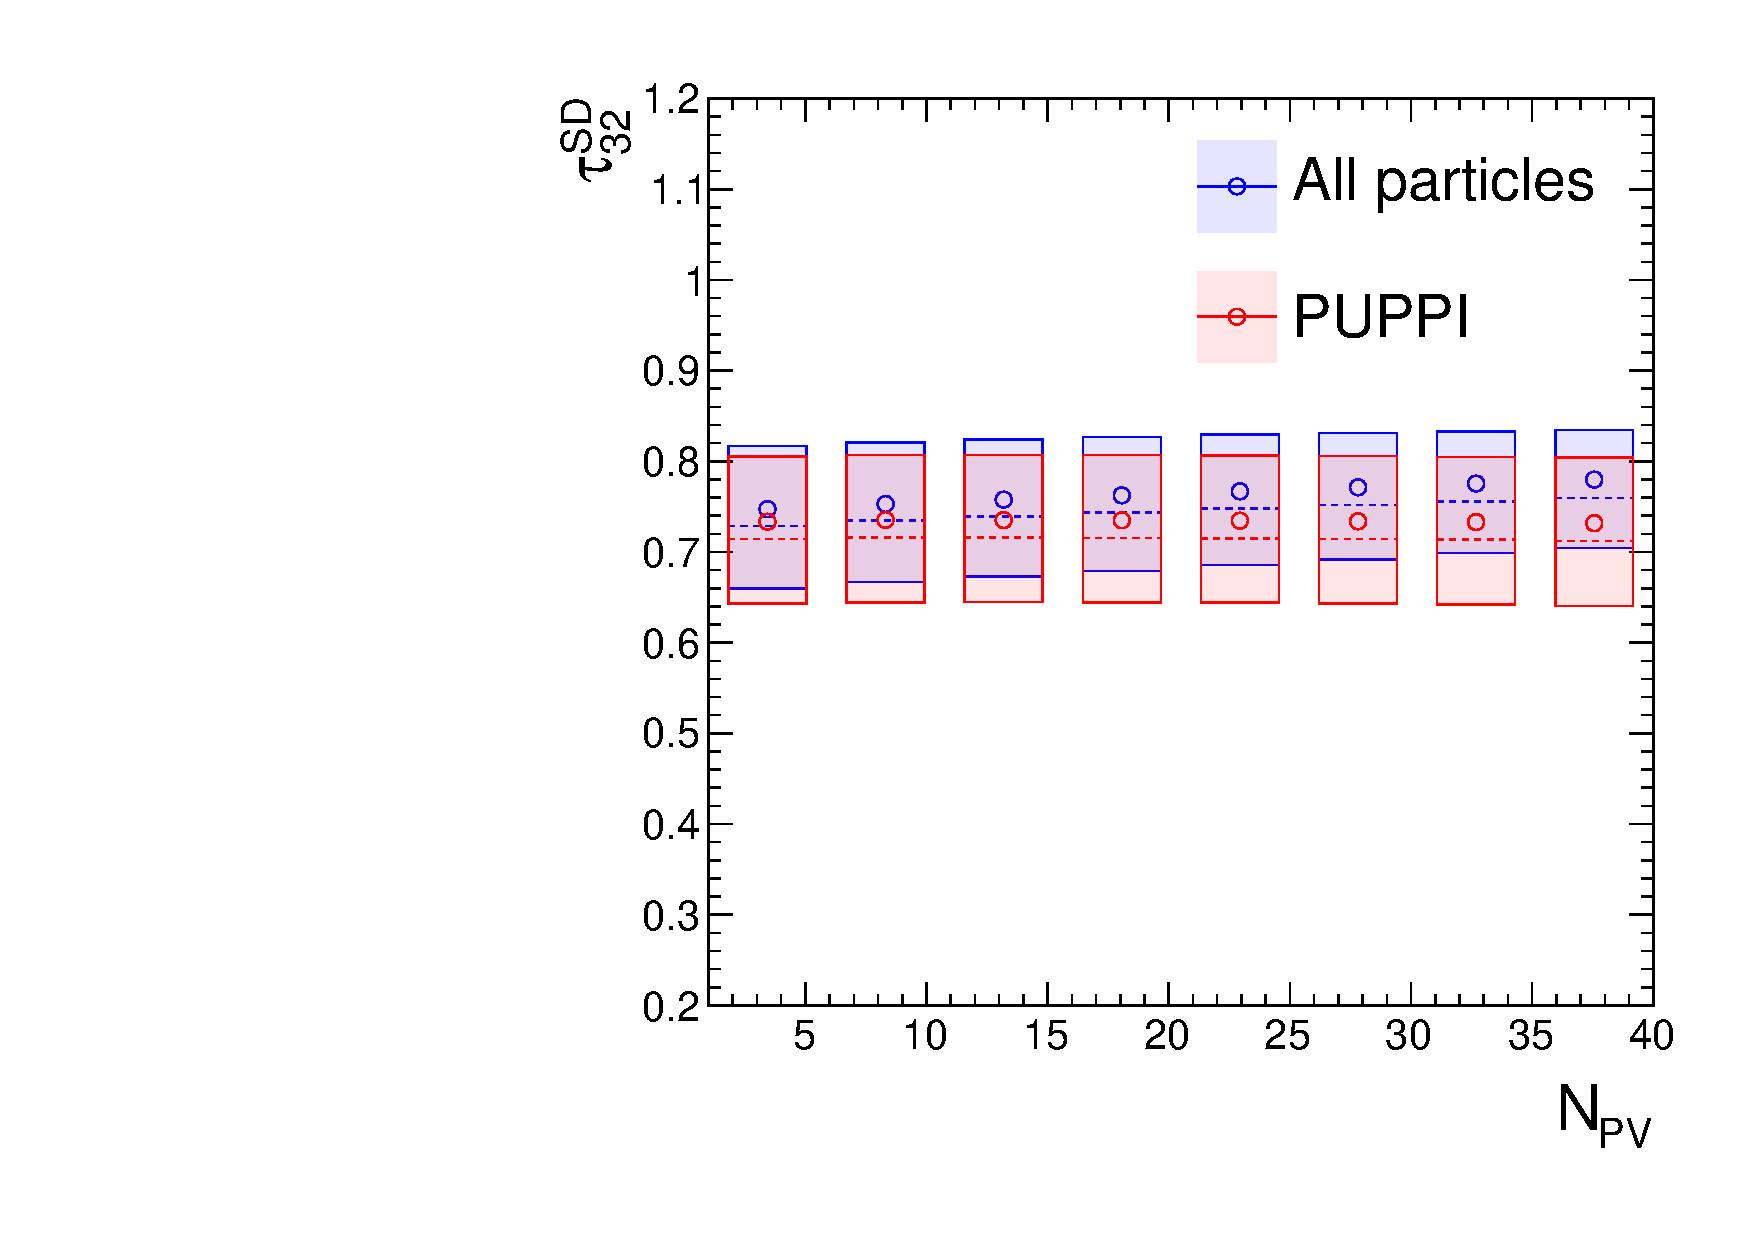
\includegraphics[width=\textwidth]{figures/toptagging/gen/npv_clf_Tau32SD_QCD.pdf}
            \caption{$\tau_{32}^\SD$, LQG}
        \end{subfigure}
        \begin{subfigure}[t]{0.35\textwidth}
            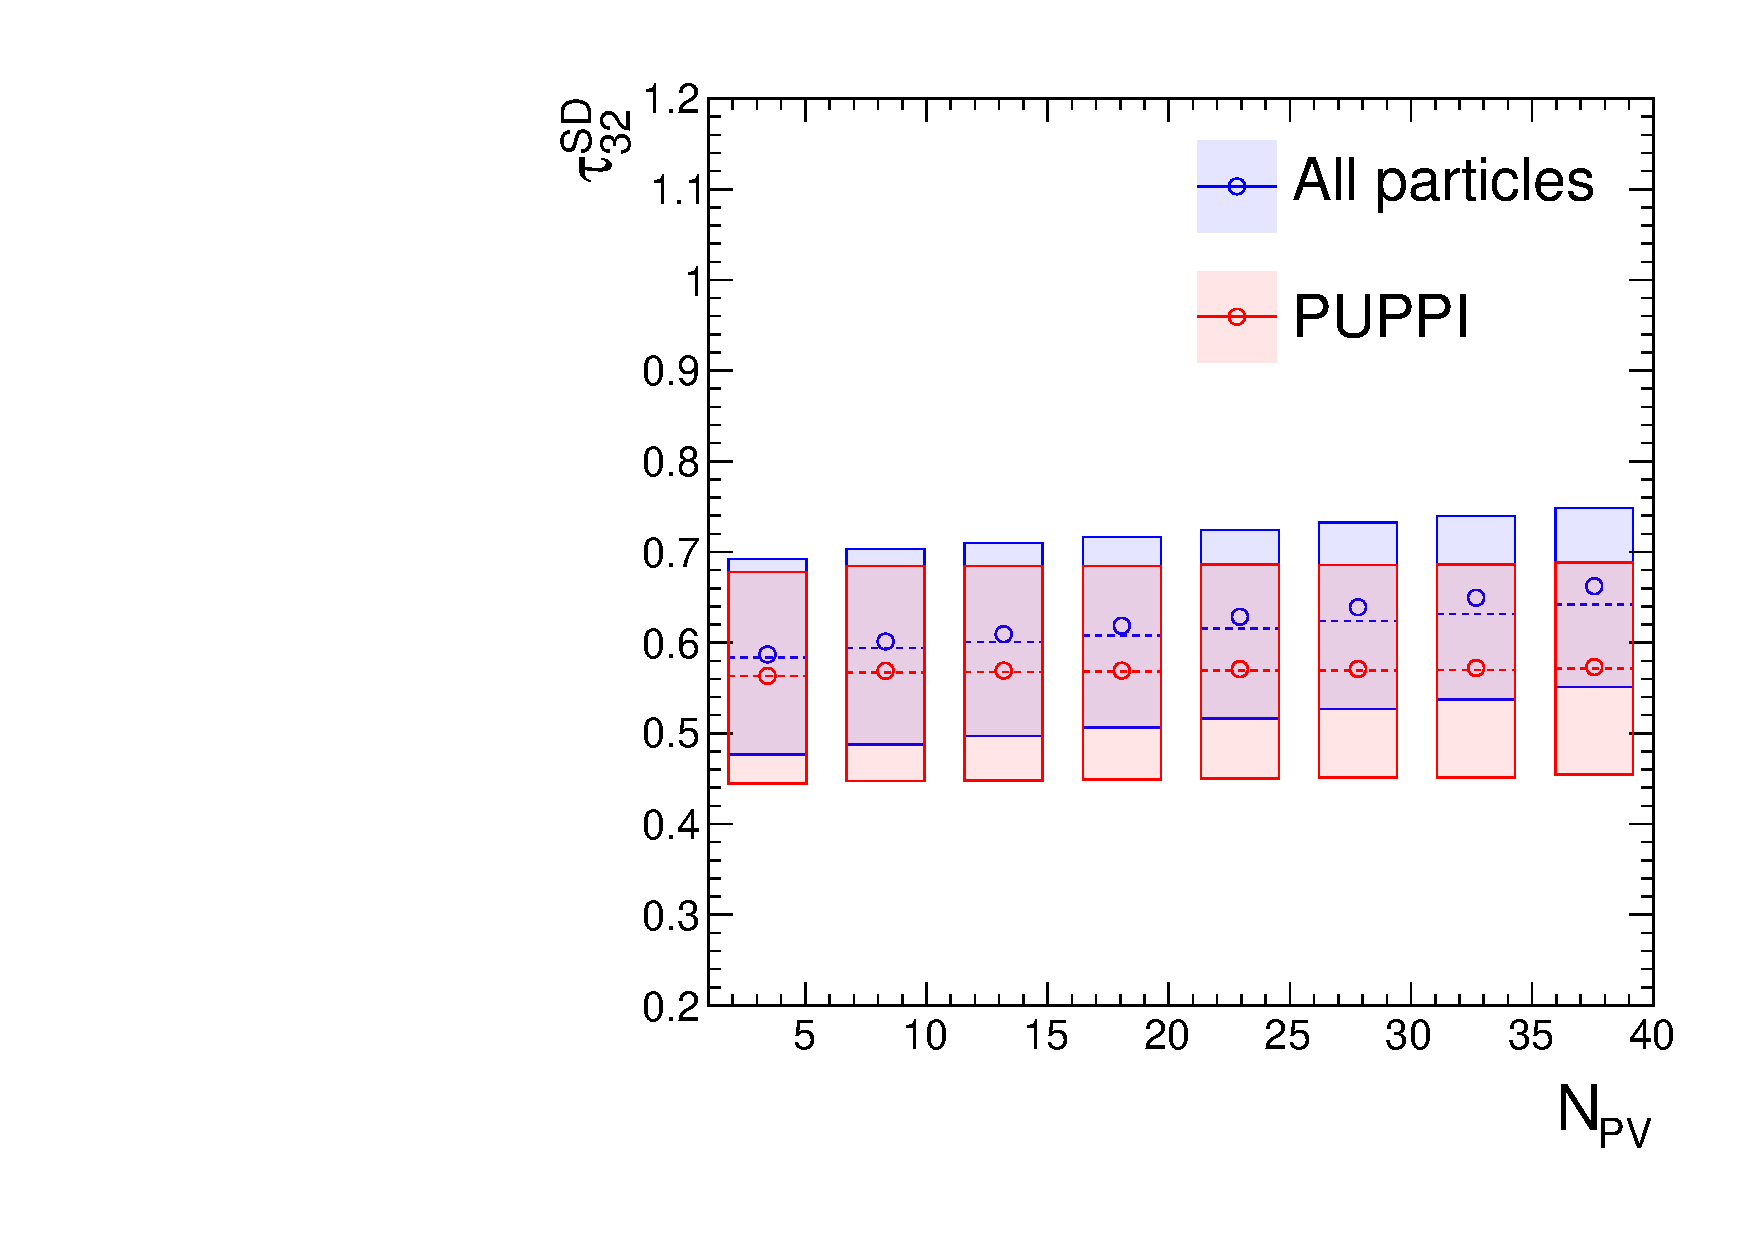
\includegraphics[width=\textwidth]{figures/toptagging/gen/npv_clf_Tau32SD_ZpTT_lo.pdf}
            \caption{$\tau_{32}^\SD$, Top}
        \end{subfigure}
        \caption{Stability of two CA15 jet observables (described in Section~\ref{sec:jets:id}) as a function of $N_\mathrm{PV}$.
            The median (mean) of each \NPV~bin is represented by an open circle (dashed line), while the $[25\%,75\%]$ percentile range is shown with a box.}
        \label{fig:jets:puppi}
    \end{center}
\end{figure}


\section{Identification}
\label{sec:jets:id}

Having reconstructed the candidate top quark jets, we turn to the problem of \emph{identifying} which CA15 jets originate from top quarks as opposed to light $q/g$ hadronization. 
As indicated in Figure~\ref{fig:jets:caak}, the jet mass is a powerful observable, but top (LQG) jets do not necessarily have a mass of $m_t$ ($m_q,m_g\sim 0$). 
While some of this discrepancy is caused by mismeasurement of the jet energy scale, a substantial fraction originates from extra radiation being absorbed into the jet.
These extra particles arise from pile-up, ISR, and underlying event (UE).
Pile-up particles are already accounted for by PUPPI.
Many algorithms exist to \emph{groom} ISR and UE particles from a jet after it has been clustered; here, we will discuss and use the soft drop (SD) method~\cite{sd}.
SD removes parts of the CA clustering tree which represent very wide-angle or asymmetric splittings, whic are atypical for a parton shower.
More formally, at each node in the clustering tree, the softer subjet of the node will be removed if it satisfies the condition:
\begin{equation}
    \frac{\min(p_\mathrm{T,1},p_\mathrm{T,2})}{p_\mathrm{T,1}+p_\mathrm{T,2}} < 
    \left(\frac{\Delta R_{12}}{R}\right)^\beta
\end{equation}
where $p_\mathrm{T,i}$ refers to the \pt~of the $i$-th subjet of the node; $\Delta R_{12}$ is the $R$-distance between the two subjets; and $R$ and $\beta$ are tunable parameters. 
This process starts at the root node of the clustering tree (i.e.~the whole jet) and proceeds iteratively to the leaves (i.e.~individual particles).
This condition is satisfied if the two subjets are very far apart (assuming $\beta \geq 0)$ or if the splitting is very asymmetric in momentum. 
We define the \emph{SD subjets} (or where clear, simply \emph{subjets}) of a jet to be the two branches of the root node, after branches failing the SD condition have been removed. 
The particles remaining after this grooming procedure are combined to make the \emph{groomed} or SD jet. 

We then define $m_\mathrm{SD}$ as the mass of the SD jet. 
Observables may also be defined in terms of the groomed or ungroomed jet. 
Figure~\ref{fig:jets:msd} compares the ungroomed and groomed mass distributions in top and LQG jets, as a function of jet momentum. 
It is immediately clear that grooming provides (a) a sharper mass peak in top jets at $m_t$ and (b) a smoothly falling mass distribution in LQG jets that goes to 0.
Furthermore, SD ensures the stability of the mass distribution as a function of jet \pt, especially in LQG jets.
For these reasons, $m_\mathrm{SD}$ will be our standard definition of jet mass. 


\begin{figure}[]
    \begin{center}
        \begin{subfigure}[t]{0.35\textwidth}
            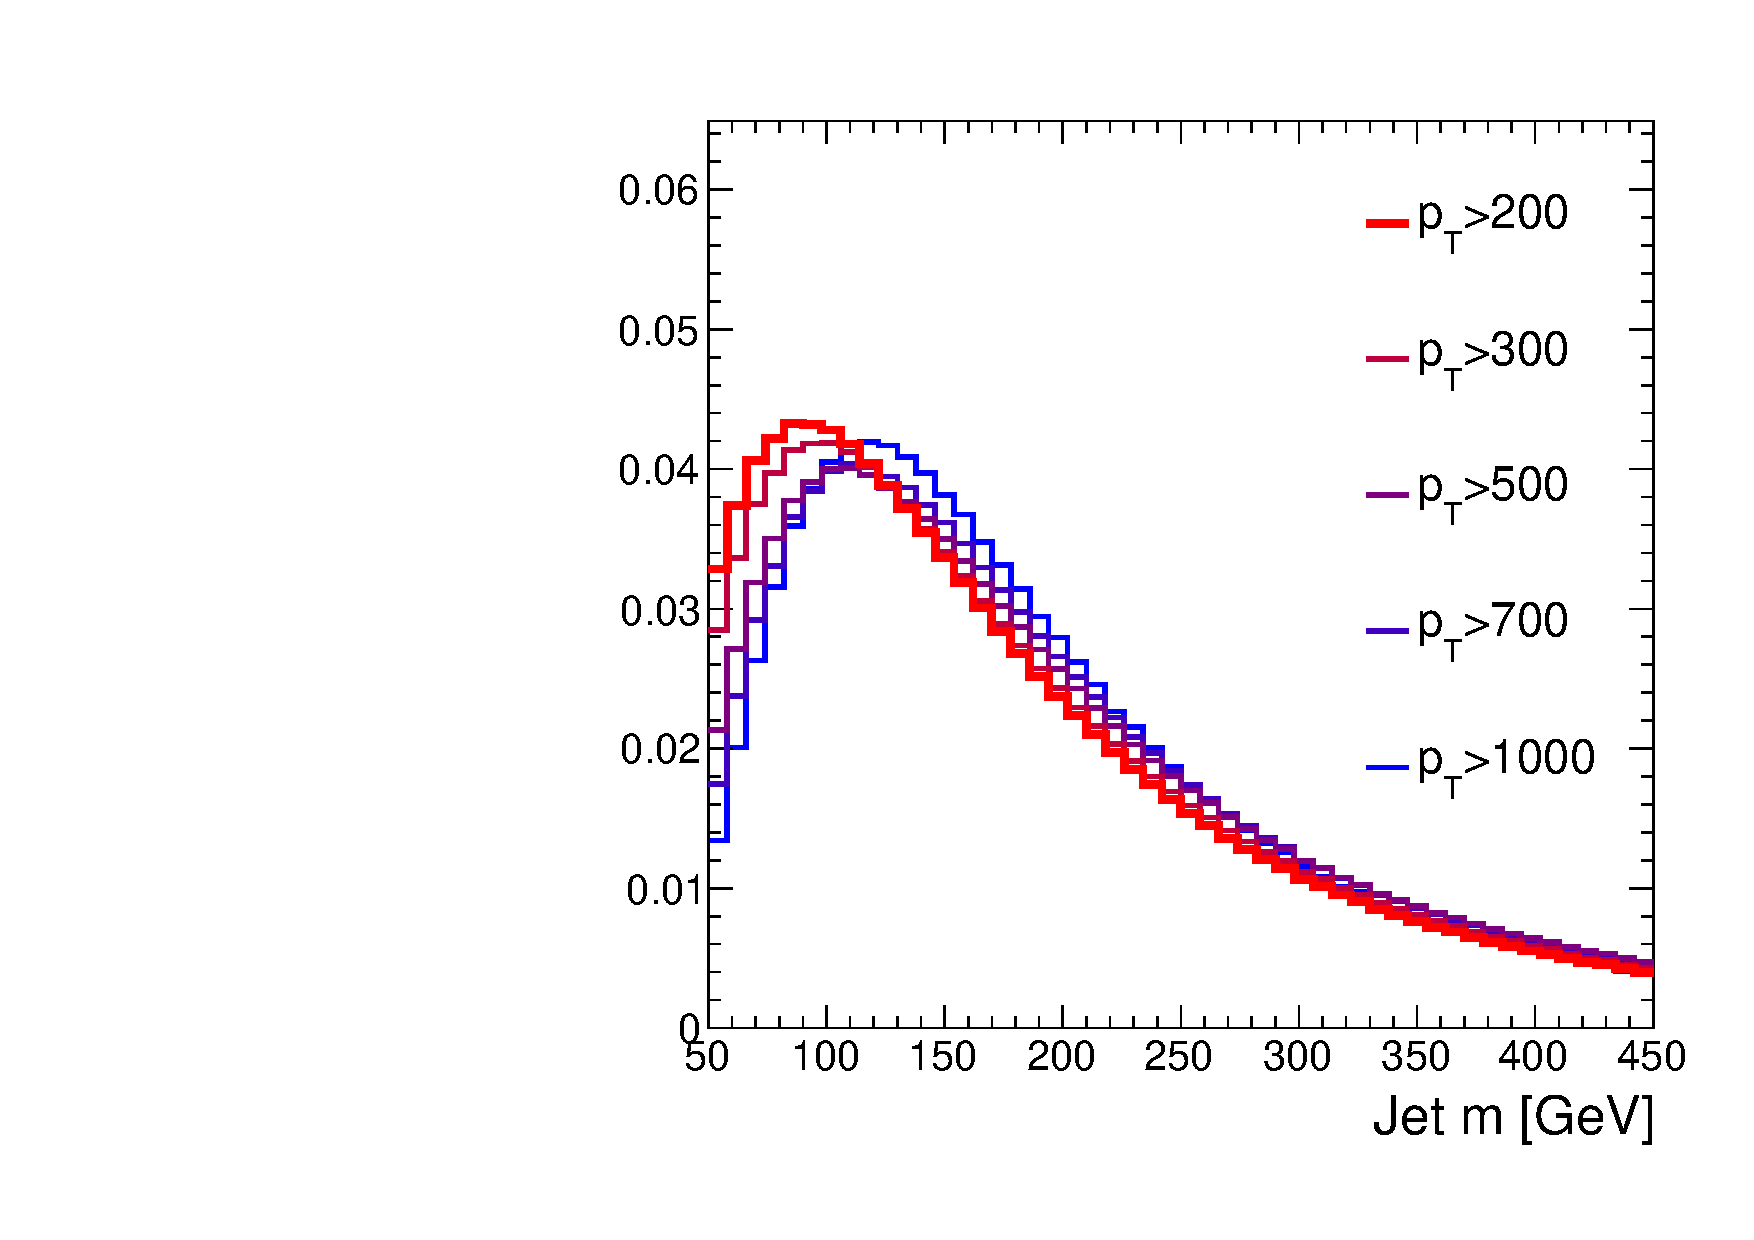
\includegraphics[width=\textwidth]{figures/toptagging/gen/norm_clf_M_QCD.pdf}
            \caption{Ungroomed, LQG}
        \end{subfigure}
        \begin{subfigure}[t]{0.35\textwidth}
            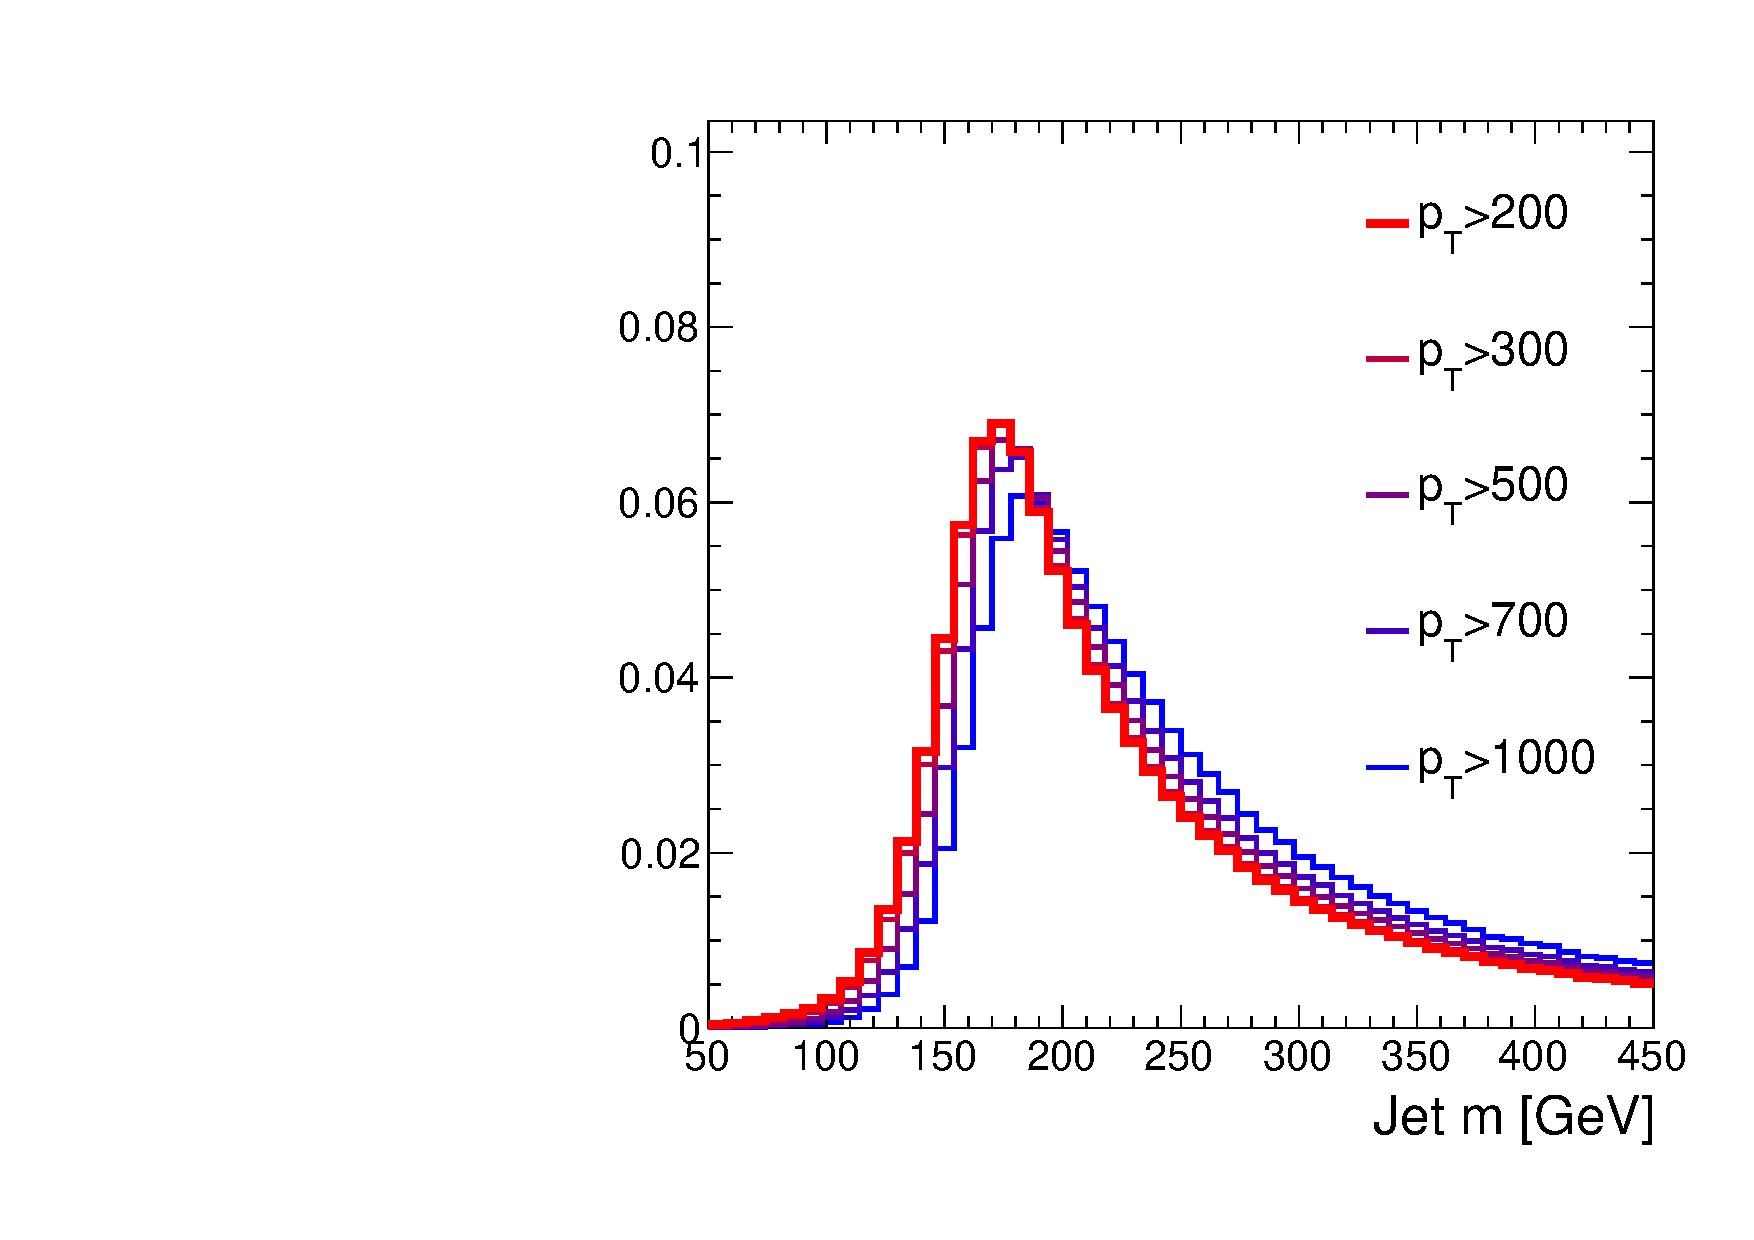
\includegraphics[width=\textwidth]{figures/toptagging/gen/norm_clf_M_ZpTT_lo.pdf}
            \caption{Ungroomed, Top}
        \end{subfigure}
        \begin{subfigure}[t]{0.35\textwidth}
            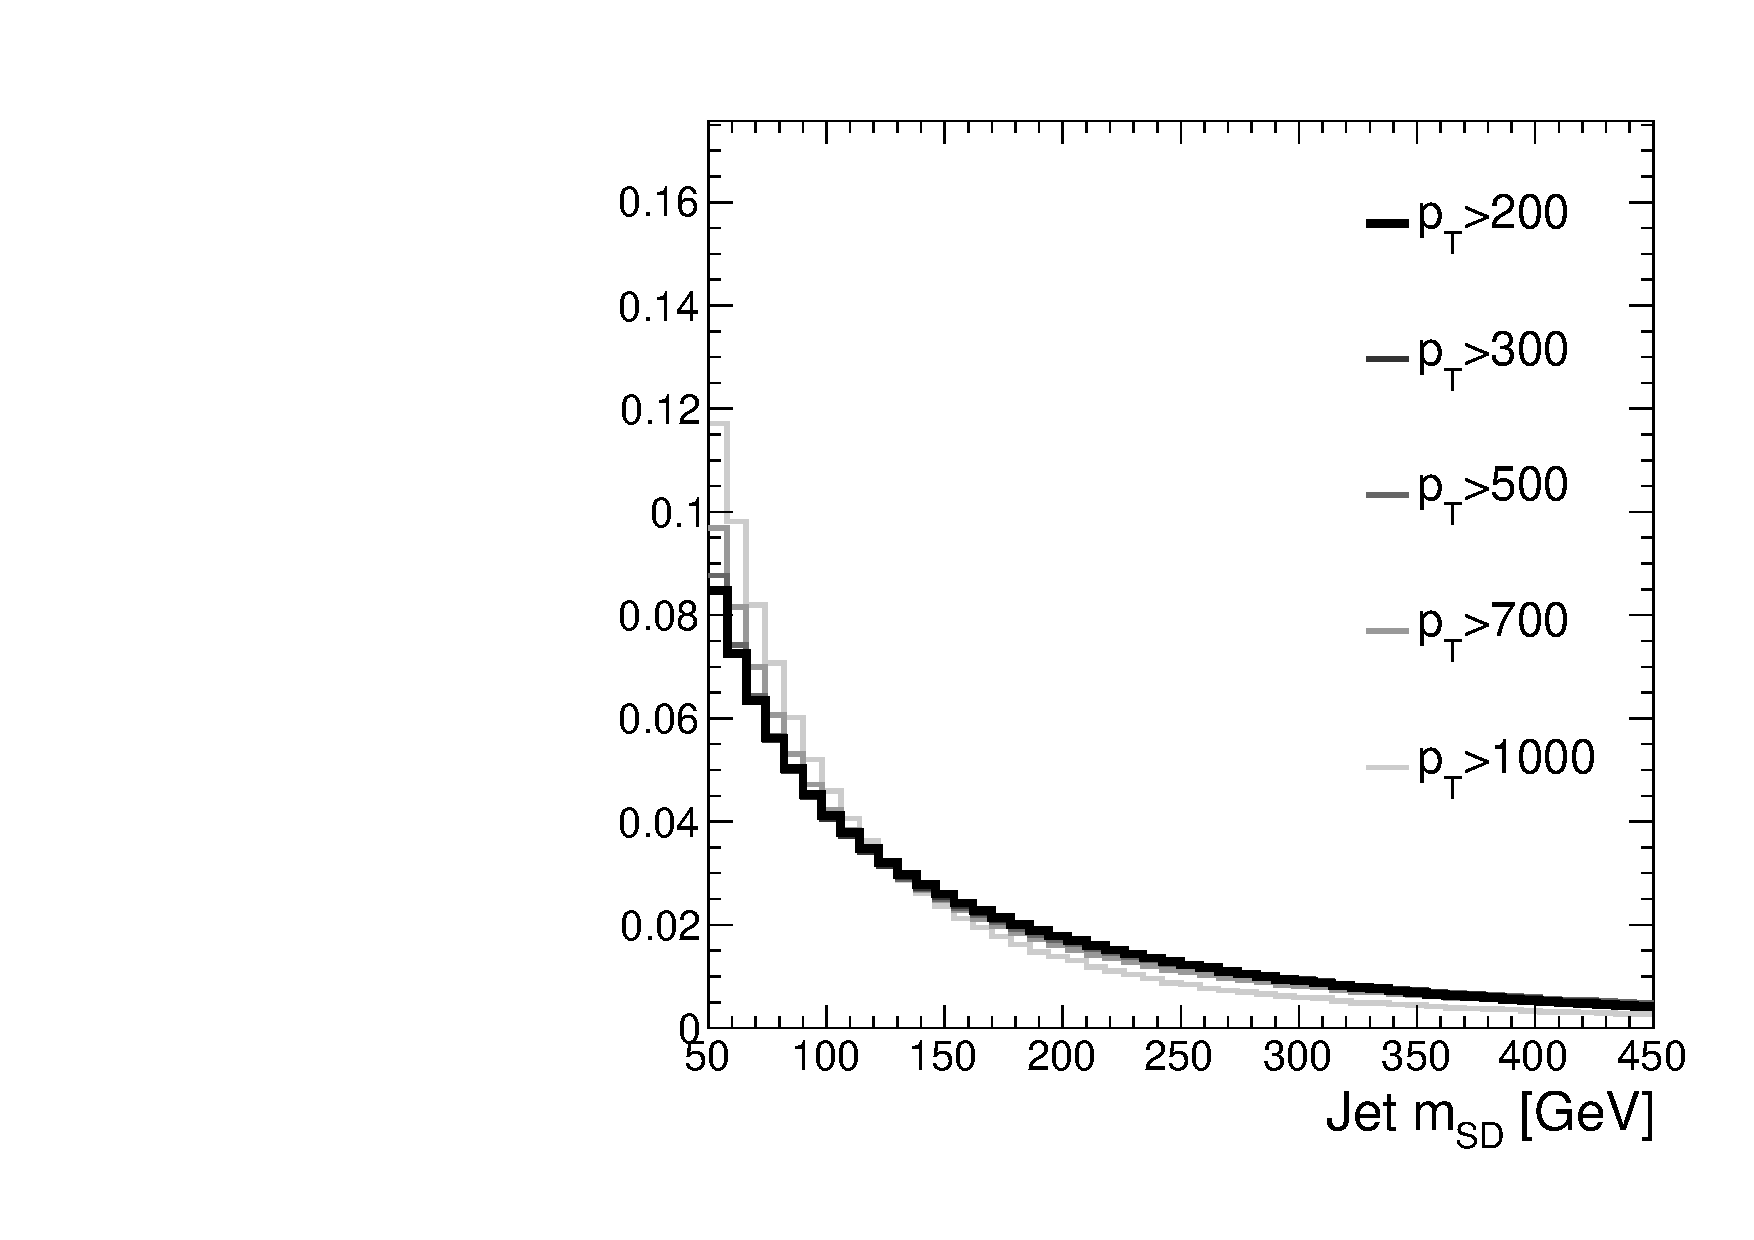
\includegraphics[width=\textwidth]{figures/toptagging/gen/norm_clf_MSD_QCD.pdf}
            \caption{SD, LQG}
        \end{subfigure}
        \begin{subfigure}[t]{0.35\textwidth}
            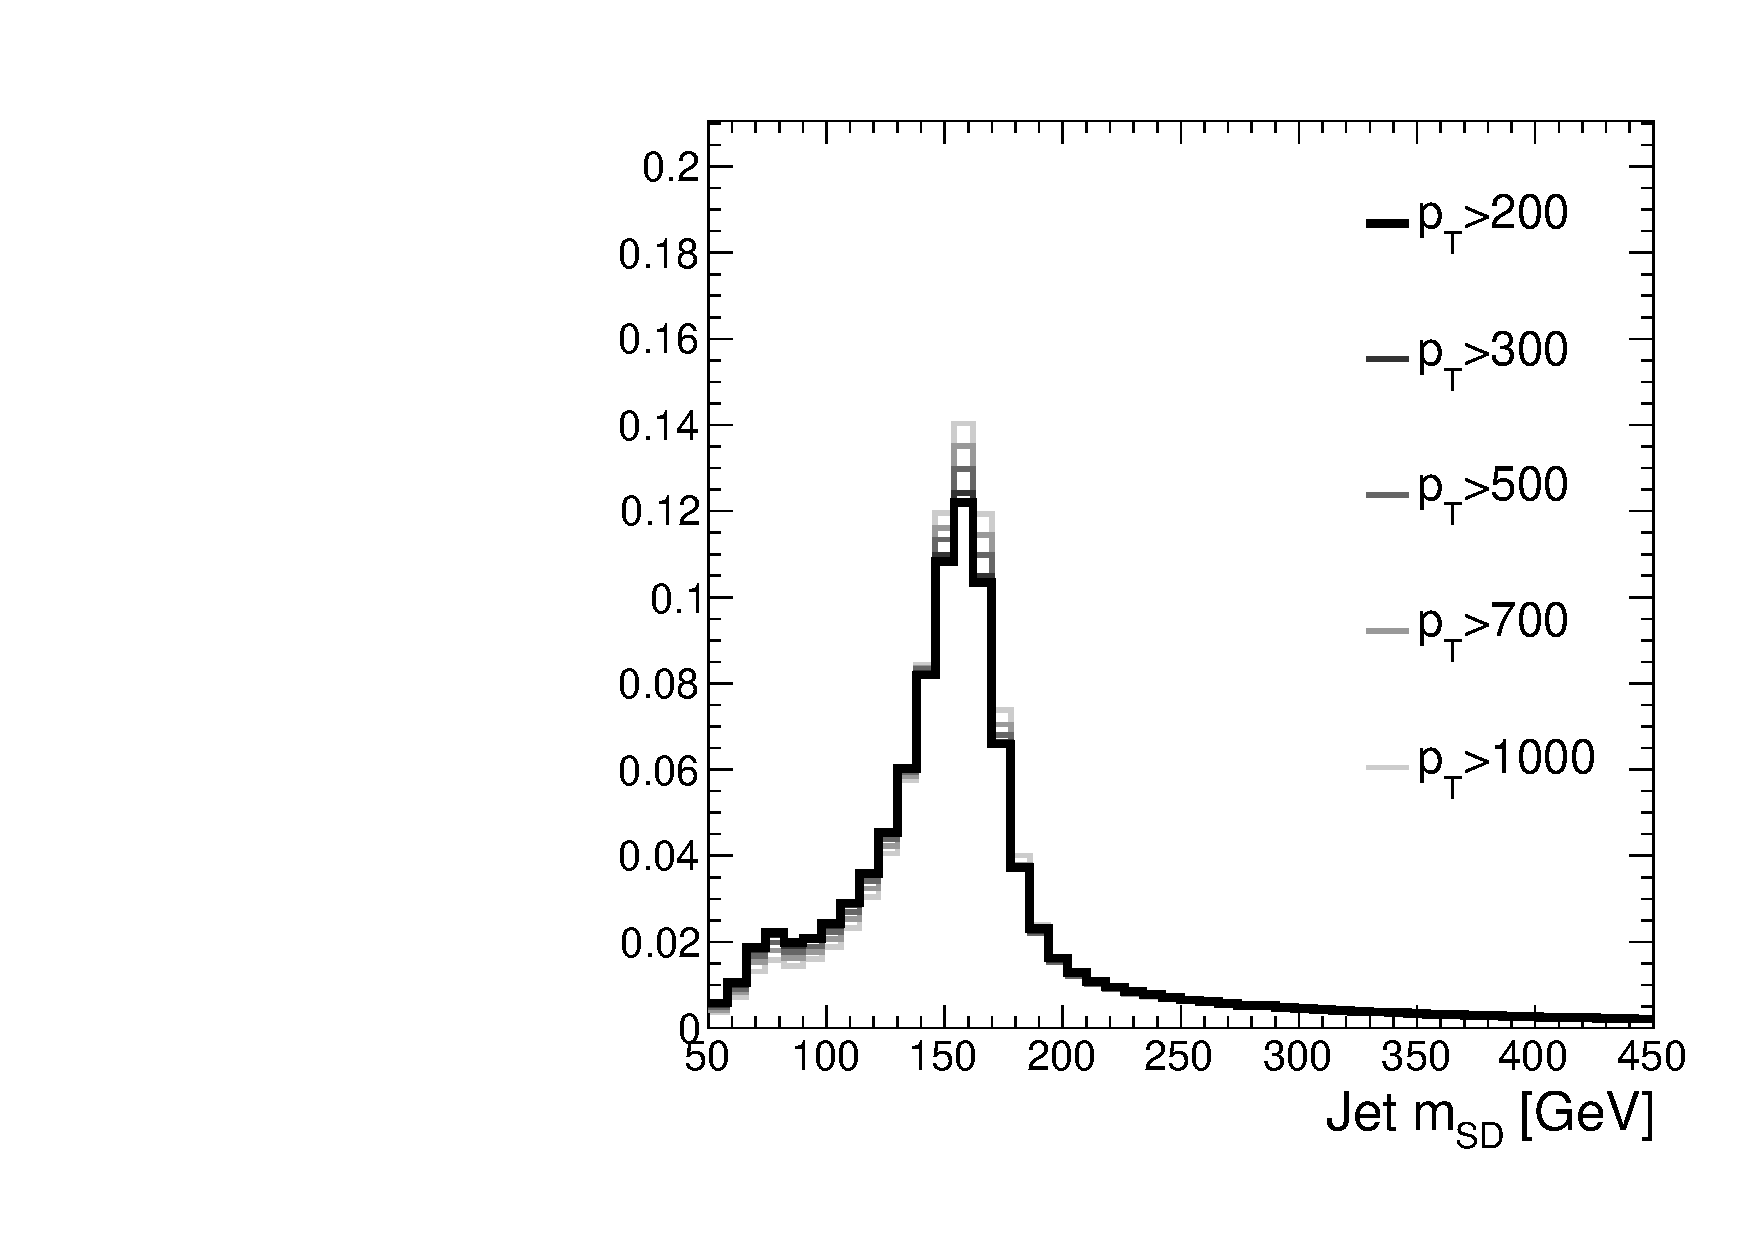
\includegraphics[width=\textwidth]{figures/toptagging/gen/norm_clf_MSD_ZpTT_lo.pdf}
            \caption{SD, Top}
        \end{subfigure}
        \caption{Distribution in simulation of ungroomed and groomed jet mass in CA15 jets originating from LQG or hadronic top decays.
                 The multiple histograms represent increasingly stringent \pt~requirements on the truth parton that initiates the jet.}
        \label{fig:jets:msd}
    \end{center}
\end{figure}

\subsection{Substructure}

A substructure observable is any function of a jet's constituents that is sensitive to the multi-pronged structure of a heavy resonance decay. 
In addition to jet mass and $b$-tagging, substructure is used to reject LQG jets as top decay candidates. 

\subsubsection{$\bm{N}$-subjettiness}

The $N$-subjettiness ($\tau_N$) is a measure of the compatibility of a jet with an $N$-axis hypothesis~\cite{nsub}.
It is defined as:
\begin{equation}
    \tau_N = \frac{\sum_{i\in\mathrm{jet}} p_{\mathrm{T},i} \min\{\Delta R_{ia} | a\in A\}}{\sum_{i\in\mathrm{jet}} p_{\mathrm{T},i} R}
    \label{eq:jets:taun}
\end{equation}
where $R=1.5$ (the jet radius); $\Delta R_{ia}$ is the $\Delta R$ distance between the particle $i$ and the axis $a$; and $A$ is a set of $N$ axes. 
Ideally, $A$ would be defined to be the set of axes that minimize $\tau_N$ for each jet, but this minimization problem is computationally difficult.  
Instead, the exclusive \kt~algorithm is used to partition the jet's constituents into $N$ subjets\footnote{These are distinct from the SD subjets discussed above.}.
The set of axes $A$ is taken to be the directions of the $N$ \kt~subjets. 
Since the \kt~distance metric is proportional to $\nicefrac{\Delta R^2}{R^2}$, this approximates the ideal minimization.
Assuming the axes are chosen to minimize Equation~\ref{eq:jets:taun}, $\tau_{N} \leq \tau_{M}$ for $N > M$. 
A small $\tau_N$ indicates a high degree of compatibility with the $N$-axis hypothesis.
Therefore, we expect a top quark jet with three prongs to satisfy $\tau_3 \ll \tau_2$, whereas a 1-pronged LQG jet should satisfy $\tau_3 \lesssim \tau_2$.
Correspondingly, we take $\tau_{32} \equiv \nicefrac{\tau_3}{\tau_2}$ to be the tagging observable. 

Figure~\ref{fig:jets:tau32} shows the distribution of $\tau_{32}$.
As with jet mass, we may calculate $\tau_{32}$ either on the whole jet or on the SD jet.
The discrimination between top and LQG jets is similar in both cases, but as Figure~\ref{fig:jets:msdtau} demonstrates, $\tau_{32}^\SD$ has the weaker correlation with $m_\SD$ in LQG jets. 
This feature will be critical to validate any tagger in data, as described in Section~\ref{sec:jets:sf}.

\begin{figure}[]
    \begin{center}
        \begin{subfigure}[t]{0.32\textwidth}
            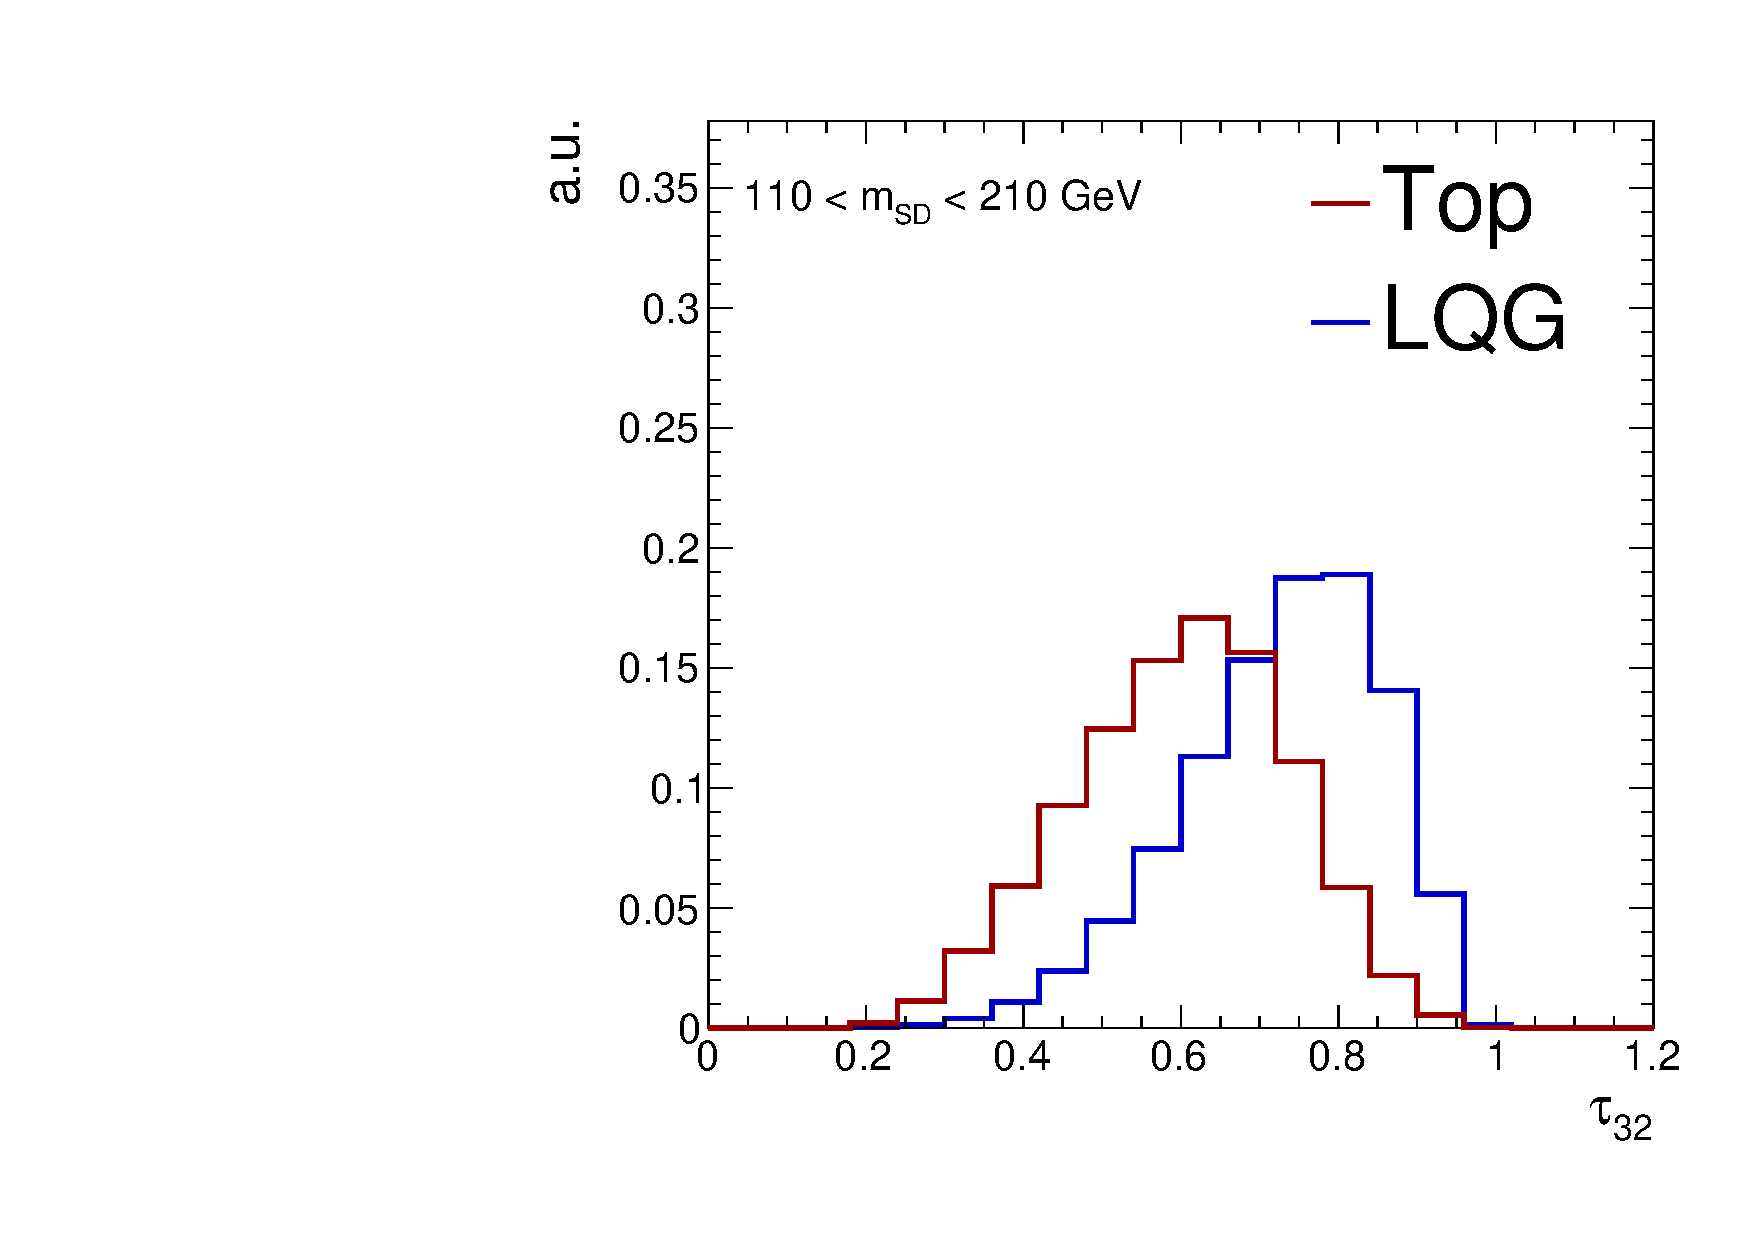
\includegraphics[width=\textwidth]{figures/toptagging/shapes/mass_fjTau32.pdf}
            \caption{}
        \end{subfigure}
        \begin{subfigure}[t]{0.32\textwidth}
            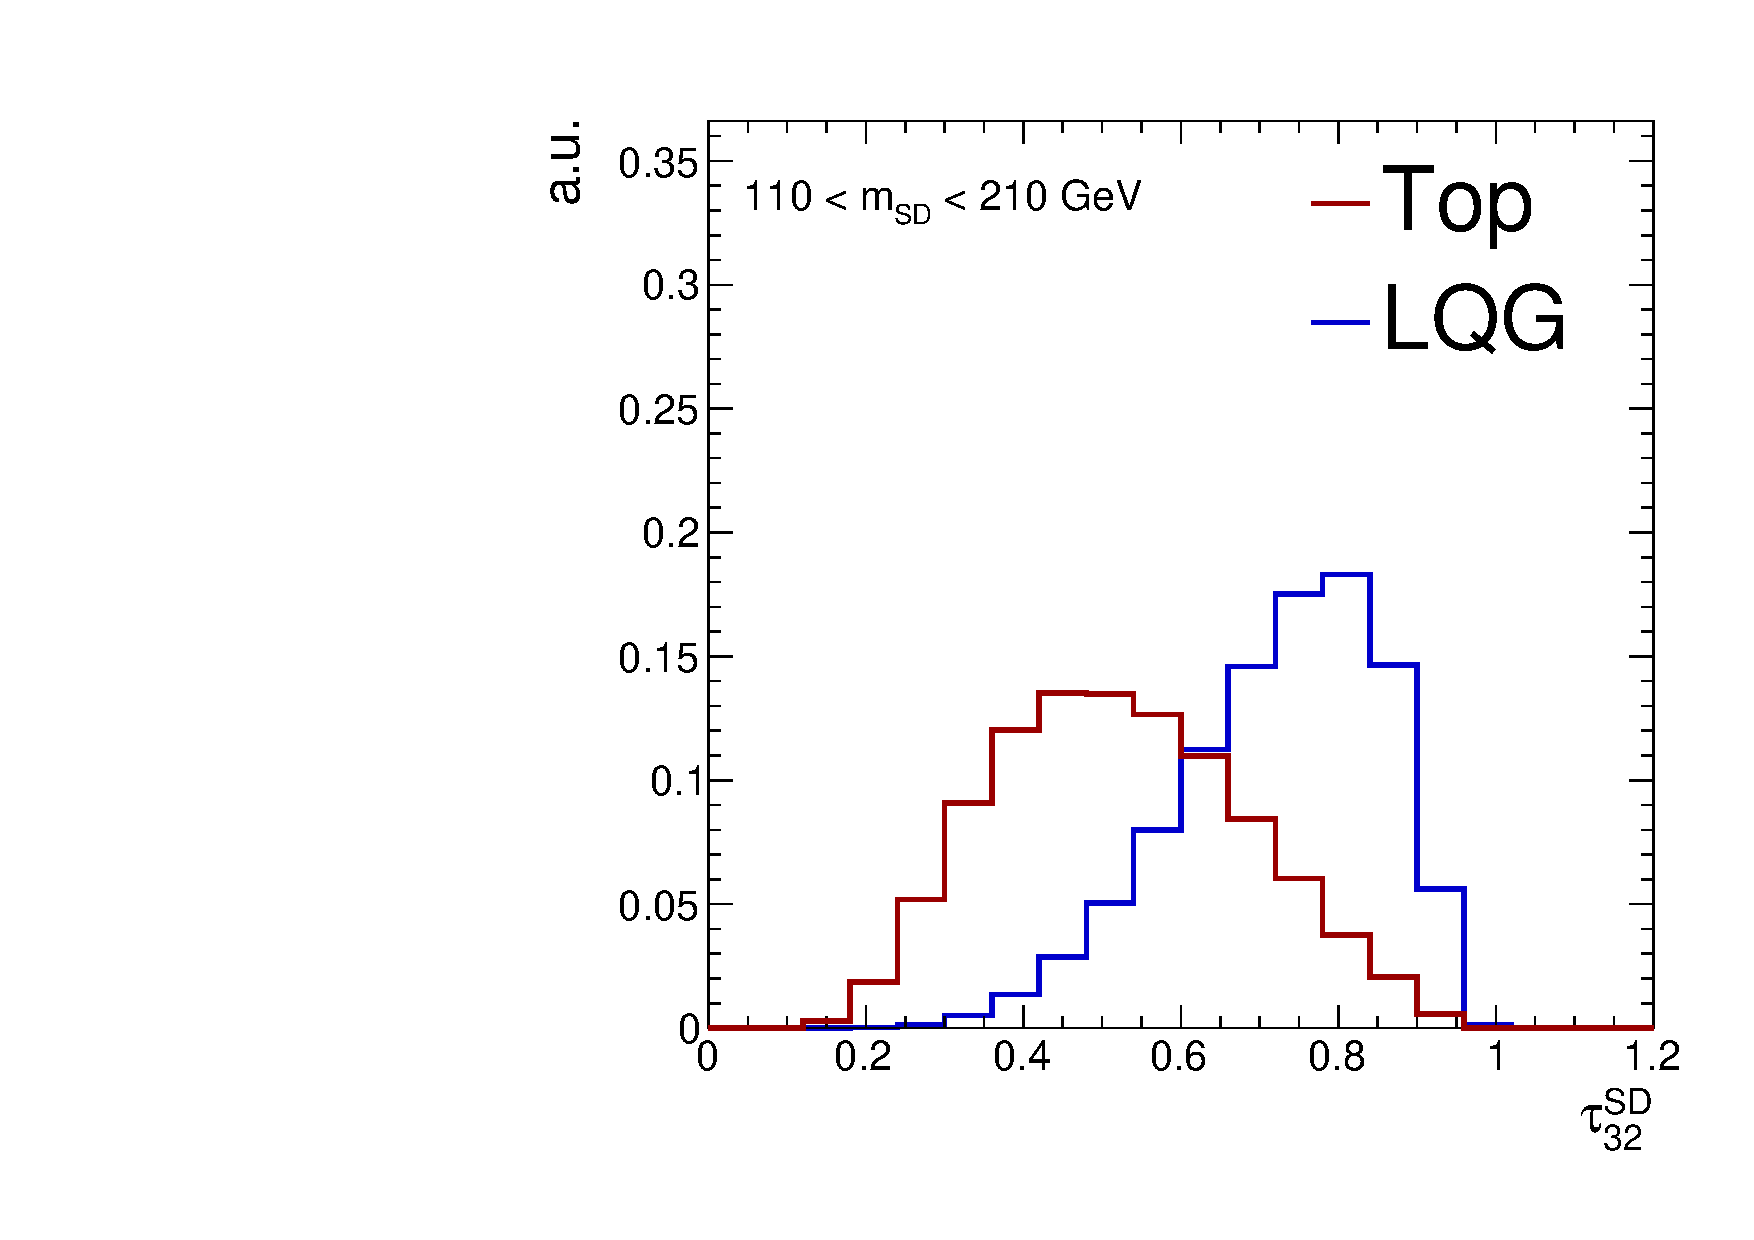
\includegraphics[width=\textwidth]{figures/toptagging/shapes/mass_fjTau32SD.pdf}
            \caption{}
        \end{subfigure}
        \begin{subfigure}[t]{0.32\textwidth}
            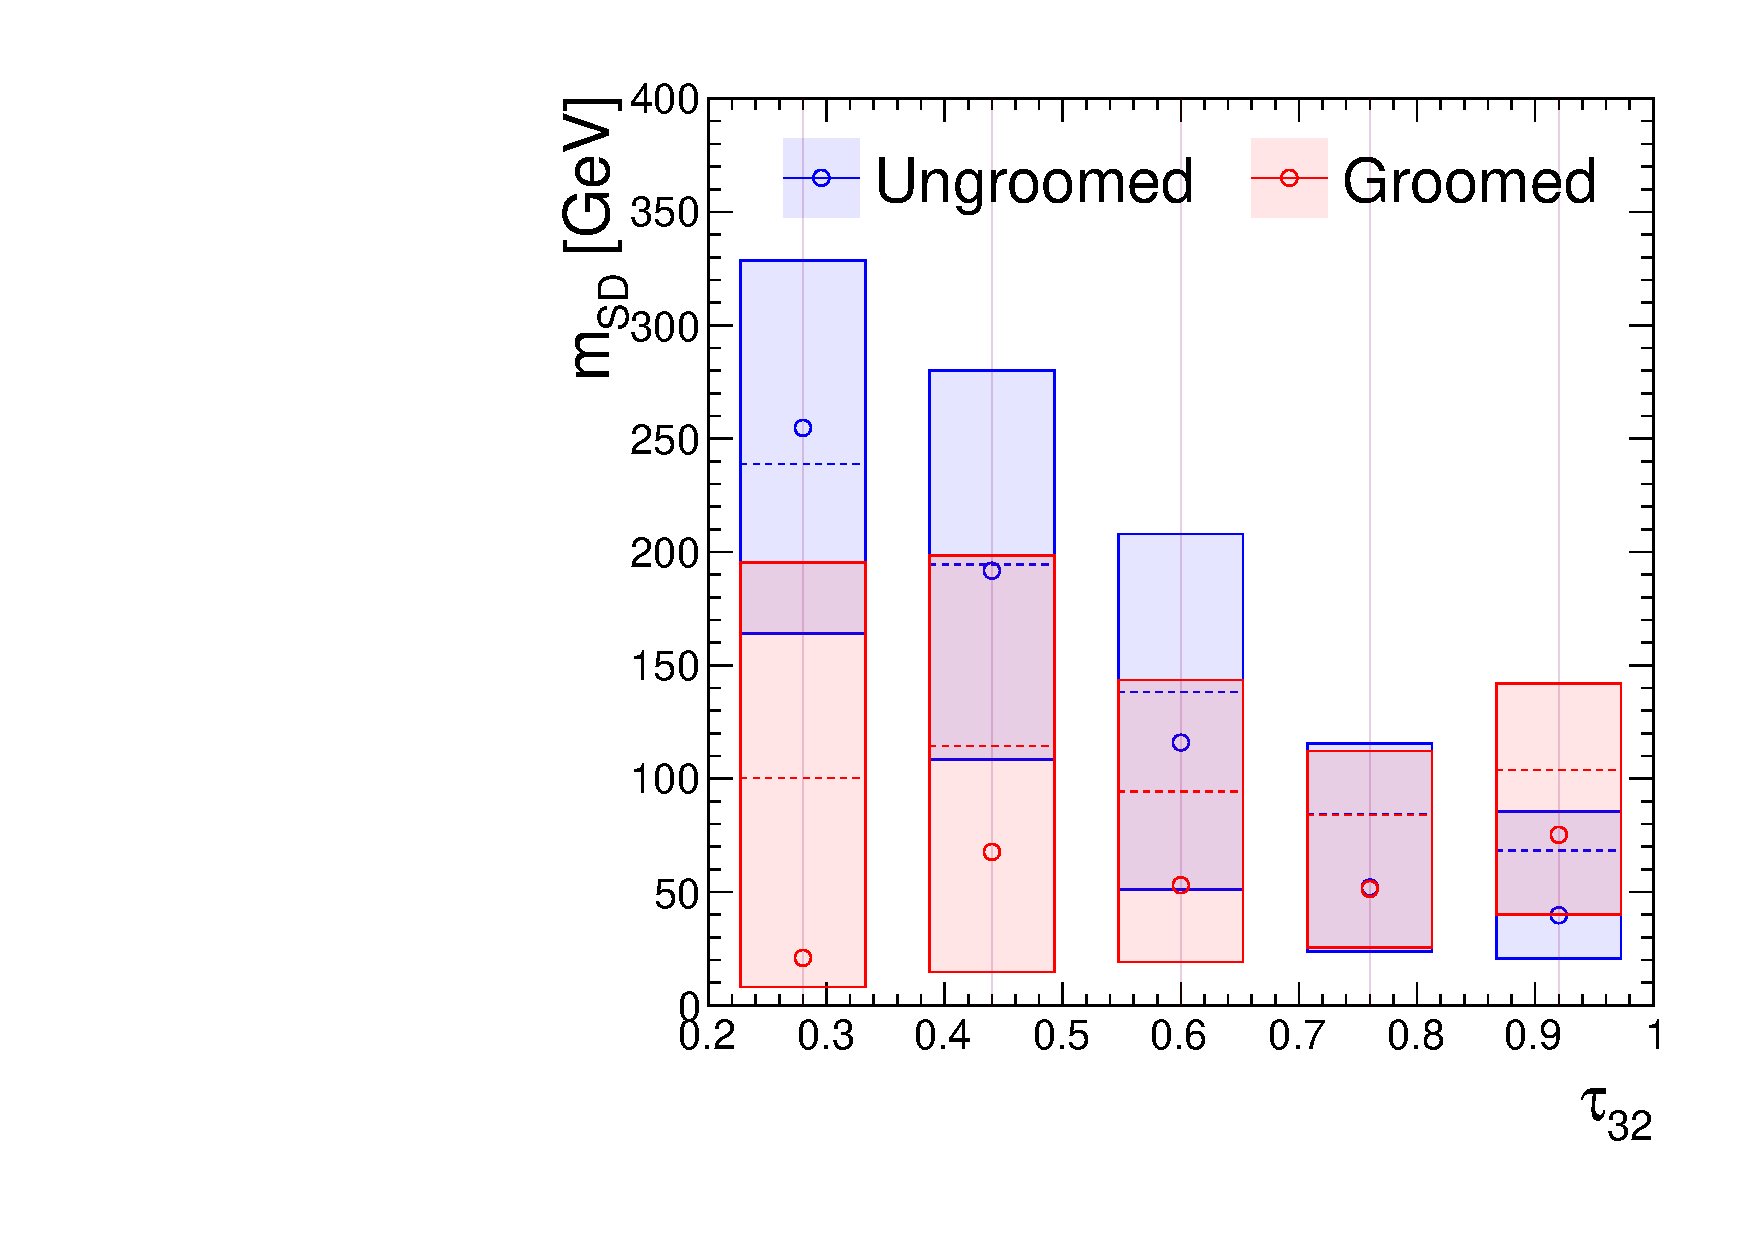
\includegraphics[width=\textwidth]{figures/toptagging/gen/msdtau_QCD.pdf}
            \caption{}
            \label{fig:jets:msdtau}
        \end{subfigure}
        \caption{Shape of ungroomed (left) and groomed (center) $\tau_{32}$ distributions in top and LQG jets, with a mass selection consistent with $m_t$. 
                 Right: the correlation between $\tau_{32}$ and $m_\SD$ in LQG jets, comparing groomed and ungroomed jets. 
                 }
        \label{fig:jets:tau32}
    \end{center}
\end{figure}

\subsubsection{\HTT}

The \HTT~algorithm de-clusters the jet into many subjets and attempts to reconstruct the $W$ and $t$ decay products out of these subjets~\cite{htt}.
The computation of the tagging variable \frec~can be simplified into three steps (a more detailed description is found in the appendix of Reference~\cite{htt}):
\begin{enumerate}
    \item Compute subjets of the CA15 jet. This is done in a fashion similar to the SD subjets discussed above, but instead of taking the two subjets of the root node, the tree is traversed until some lower \pt~bound is crossed.
    \item Test all triplet combinations of the found subjets and define the $m_{123}$ as the groomed mass of the trijet system. 
    \item Choosing the triplet most consistent with a 3-body top decay (see Equation 12 in Reference~\cite{htt}), define:
        \begin{equation}
            \frec = \min_{0\leq i < j \leq 2} \left|
            \frac{\nicefrac{m_{ij}}{m_{123}}}{\nicefrac{m_W}{m_t}} - 1\right|
        \end{equation}
        where the indices $i,j$ index elements of the selected triplet. 
\end{enumerate}
Figure~\ref{fig:jets:htt} shows the distribution of the selected $m_{123}$ and $\frec$, although we will only use the latter as a tagging observable. 
Note that we do not define distinct groomed and ungroomed versions of these observables, as grooming is already applied when defining subjets. 

\begin{figure}[]
    \begin{center}
        \begin{subfigure}[t]{0.35\textwidth}
            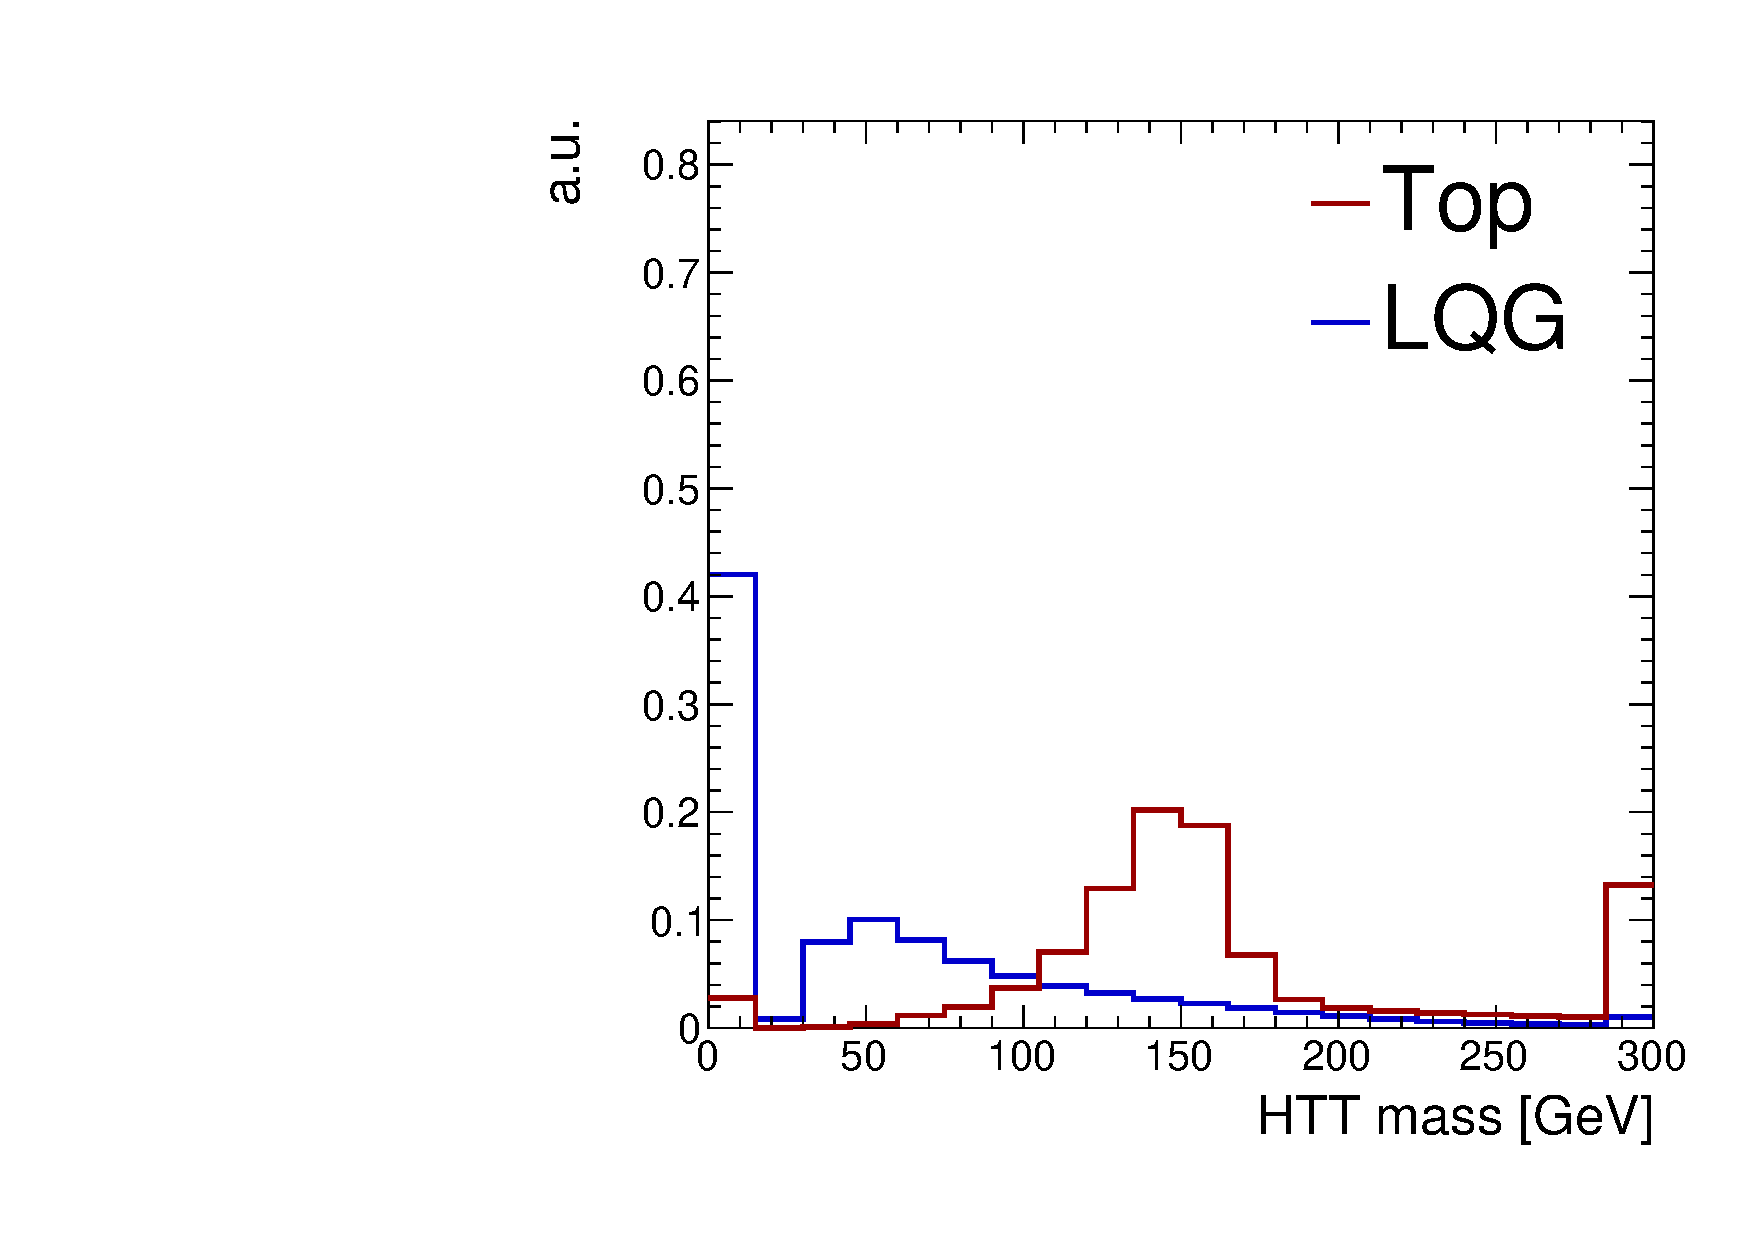
\includegraphics[width=\textwidth]{figures/toptagging/shapes/incl_fjHTTMass.pdf}
        \end{subfigure}
        \begin{subfigure}[t]{0.35\textwidth}
            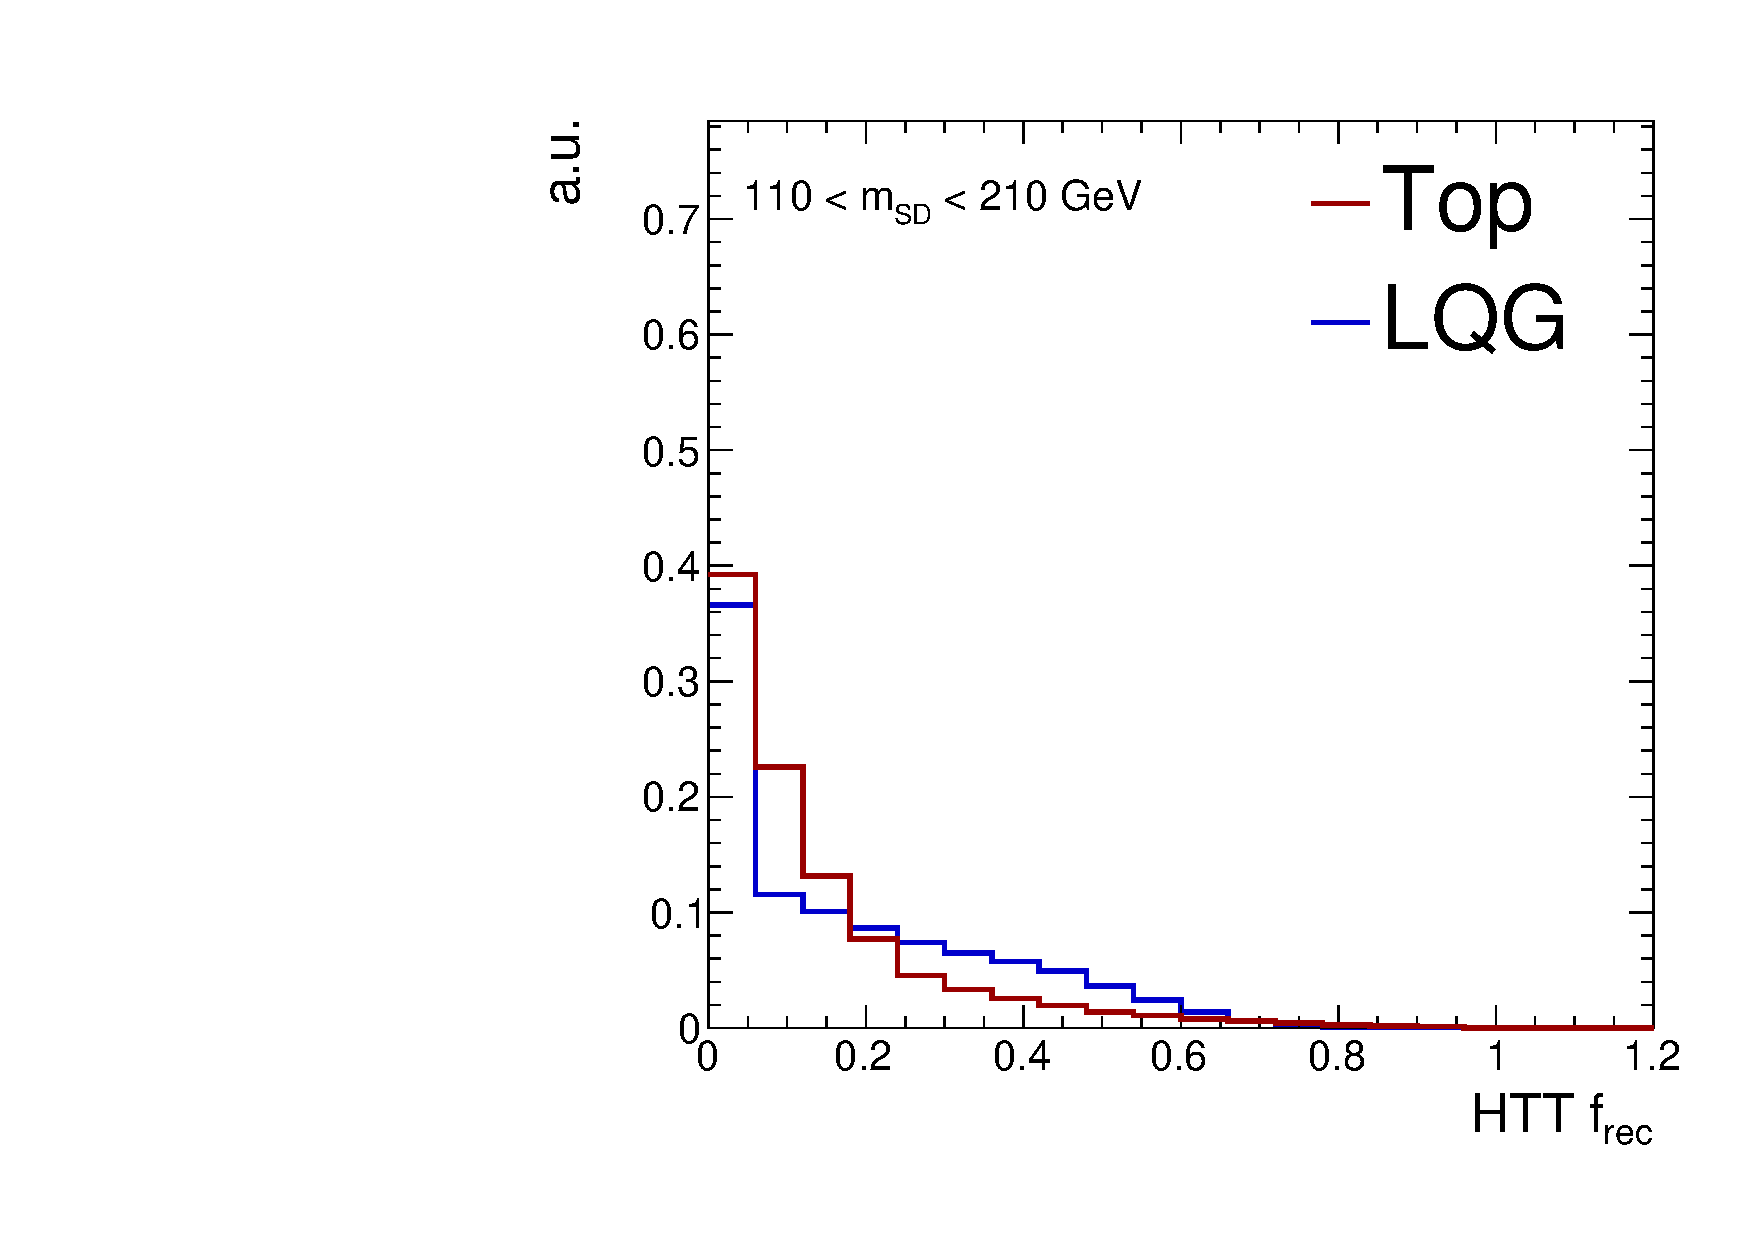
\includegraphics[width=\textwidth]{figures/toptagging/shapes/mass_fjHTTFRec.pdf}
        \end{subfigure}
        \caption{Shape of the $m_{123}$ and $\frec$ observables computed by the \HTT~algorithm. 
                 The value $m_{123} = 0$ indicates the cases in which a subjet triplet consistent with a top decay could not be found. }
        \label{fig:jets:htt}
    \end{center}
\end{figure}

\subsubsection{Energy Correlation Functions}

Energy correlation functions measure the correlation of the positions of hard particles in a jet~\cite{ecf}. 
Heuristically, an $N$-point ECF is small if the hard particles can be grouped into fewer than $N$ prongs and large if they arise from $N$ or more prongs. 
An $N$-point ECF, with angular parameters $o$ and $\beta$, is defined as:
\begin{equation}
    e(o,N,\beta) \equiv 
    ~_o e_N^\beta = 
    \sum _{K\subset J,\,|K|=N} 
    \left[\prod_{i\in K} \frac{\pt^{(i)}}{\pt^{(J)}}\right] \times 
    \min\left\{ \prod_{i,j\in P} \Delta R_{ij}^\beta 
        ~\Big|~ P \subset \tilde{K}^2 ,~|P|=o\right\}
\end{equation}
where $0 < o \leq N^2-N$ and $\tilde K^2$ indicates all pairs of distinct particles in $K$. 
The proposed tagger in Reference~\cite{ecf} is:
\begin{equation}
    N_3^{(\beta)} = \frac{e(2,4,\beta)}{(e(1,3,\beta))^2}
\end{equation}
Figure~\ref{fig:jets:n3} shows $N_3$ for various values of $\beta$; given our desire for stability as a function of jet \pt~and mass, we only consider ECFs computed on the SD jet. 
The discrimination power of this ECF ratio is roughly comparable to that of $\tau_{32}^\SD$. 
$N_3$ is motivated by the behavior of 3- and 4-point ECFs in top and LQG jets:
\begin{itemize}
    \item In top jets, $e(N=4) \ll e(N=3)$, since 3-point correlation functions are large in a 3-pronged jet
    \item In QCD jets, $e(N=3) \sim e(N=3)$, since both 3- and 4-point ECFs are weak in a 1-pronged jet
\end{itemize}
Therefore, taking the ratio $e(N=4)/e(N=3)$ constructs a useful observable. 

\begin{figure}[]
    \begin{center}
        \begin{subfigure}[t]{0.32\textwidth}
            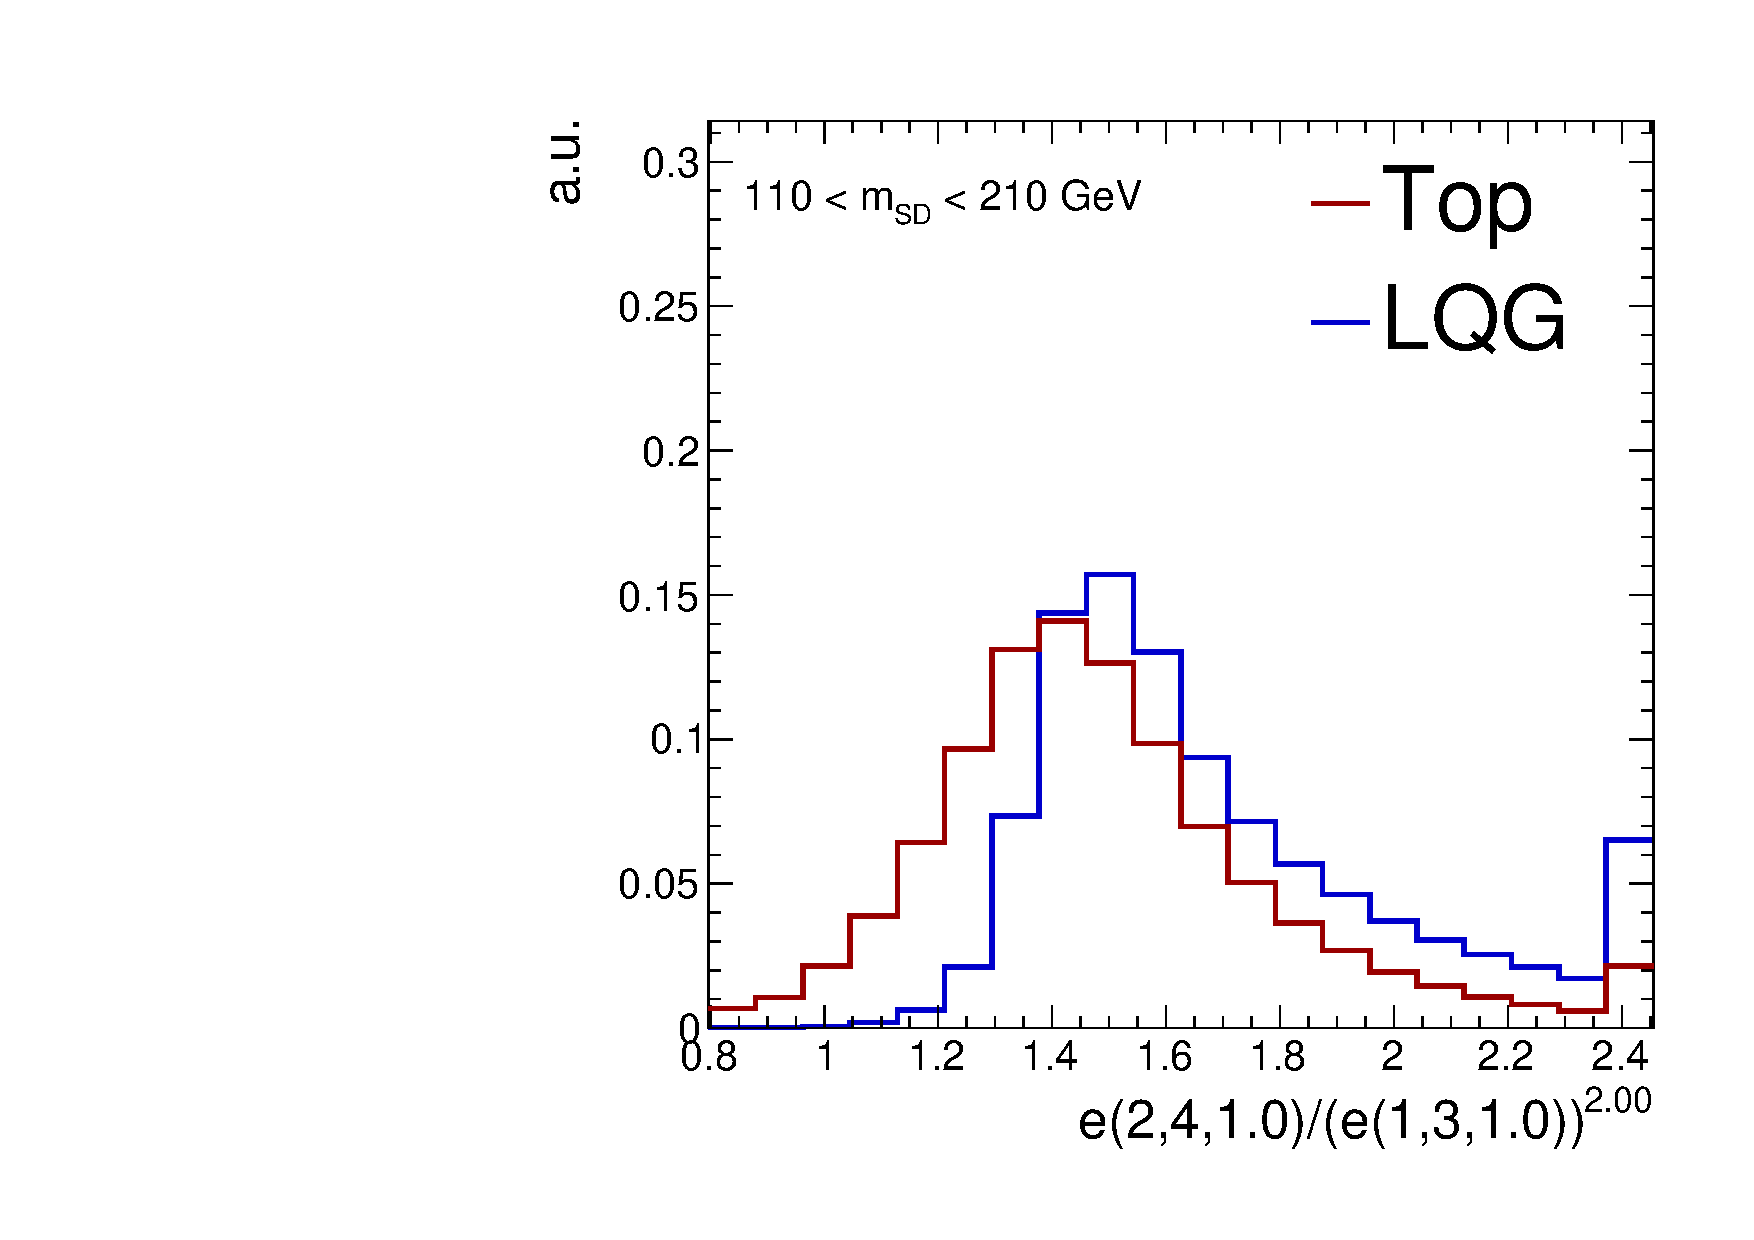
\includegraphics[width=\textwidth]{figures/toptagging/shapes/mass_ratio_24101310.pdf}
        \end{subfigure}
        \begin{subfigure}[t]{0.32\textwidth}
            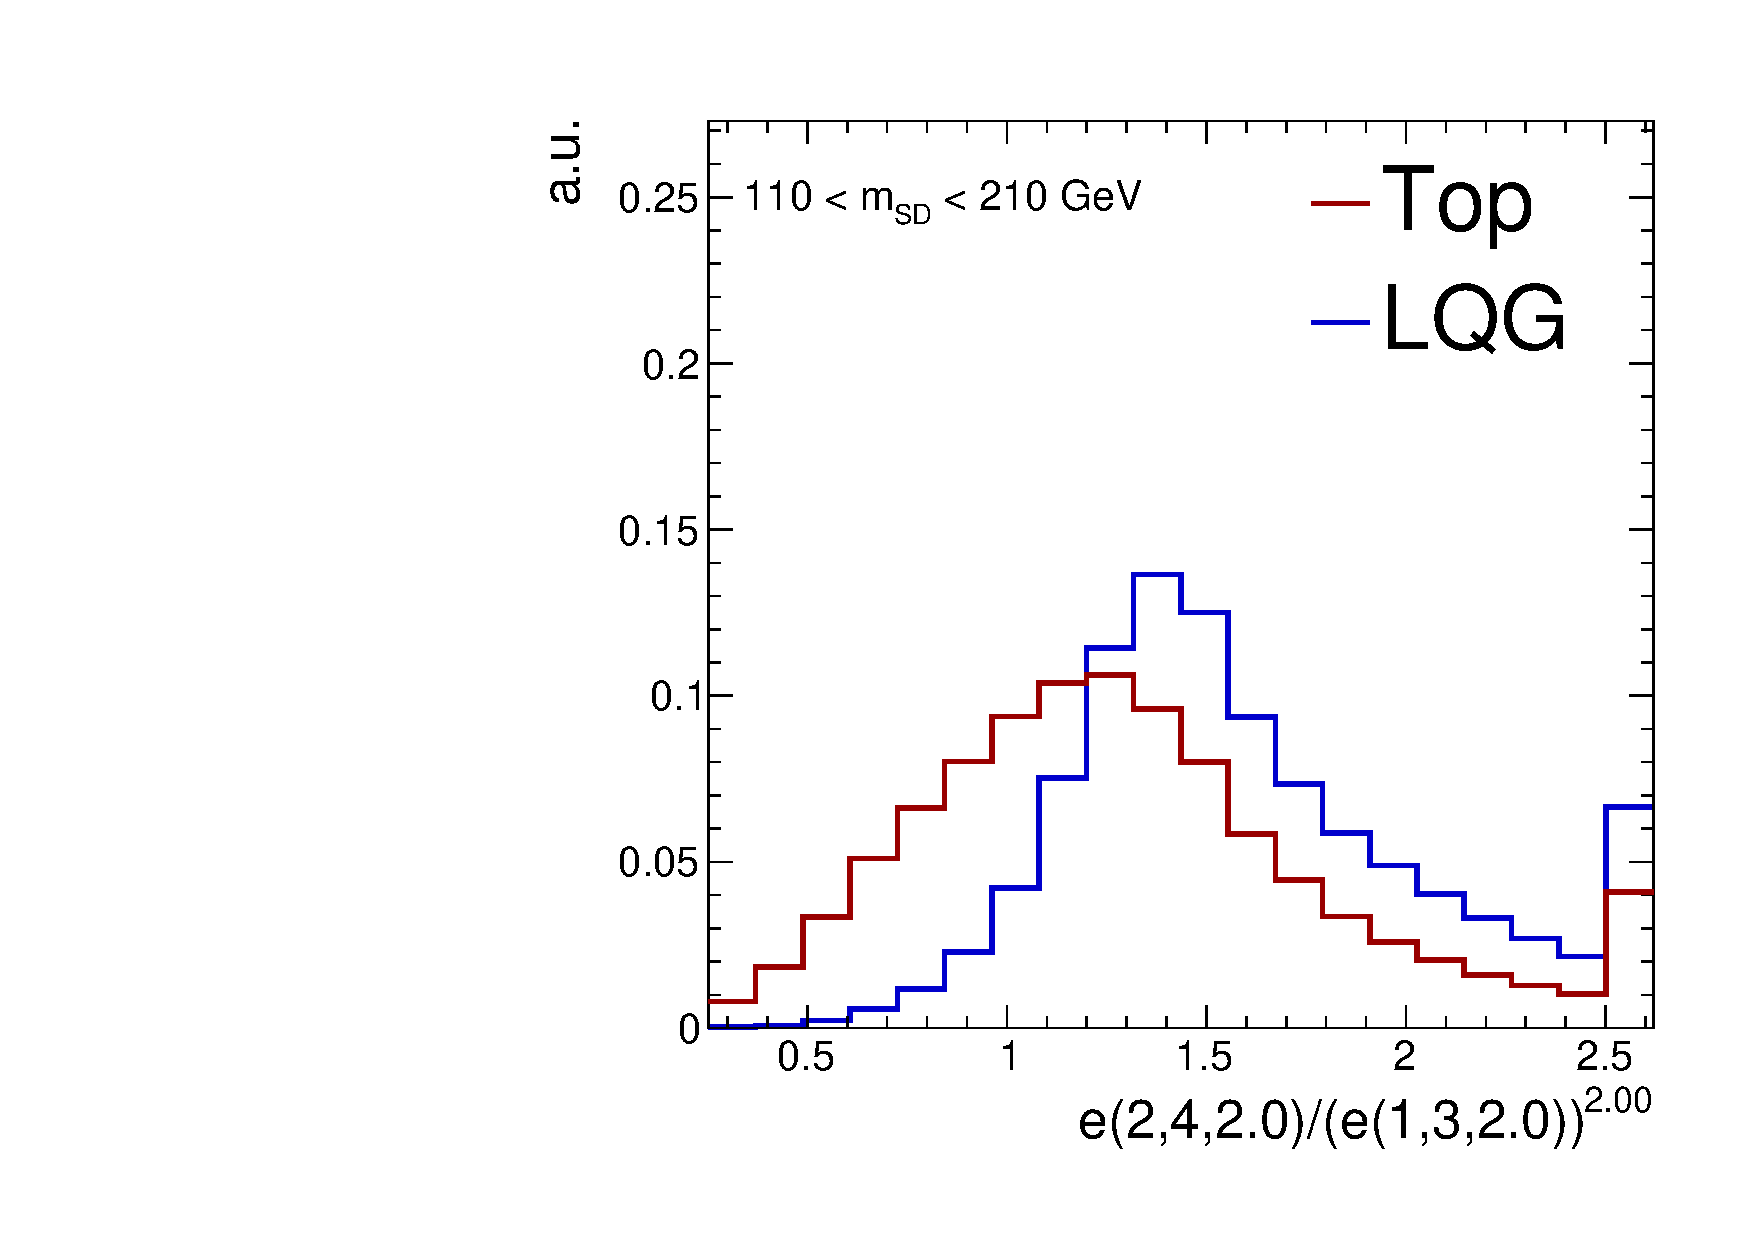
\includegraphics[width=\textwidth]{figures/toptagging/shapes/mass_ratio_24201320.pdf}
        \end{subfigure}
        \begin{subfigure}[t]{0.32\textwidth}
            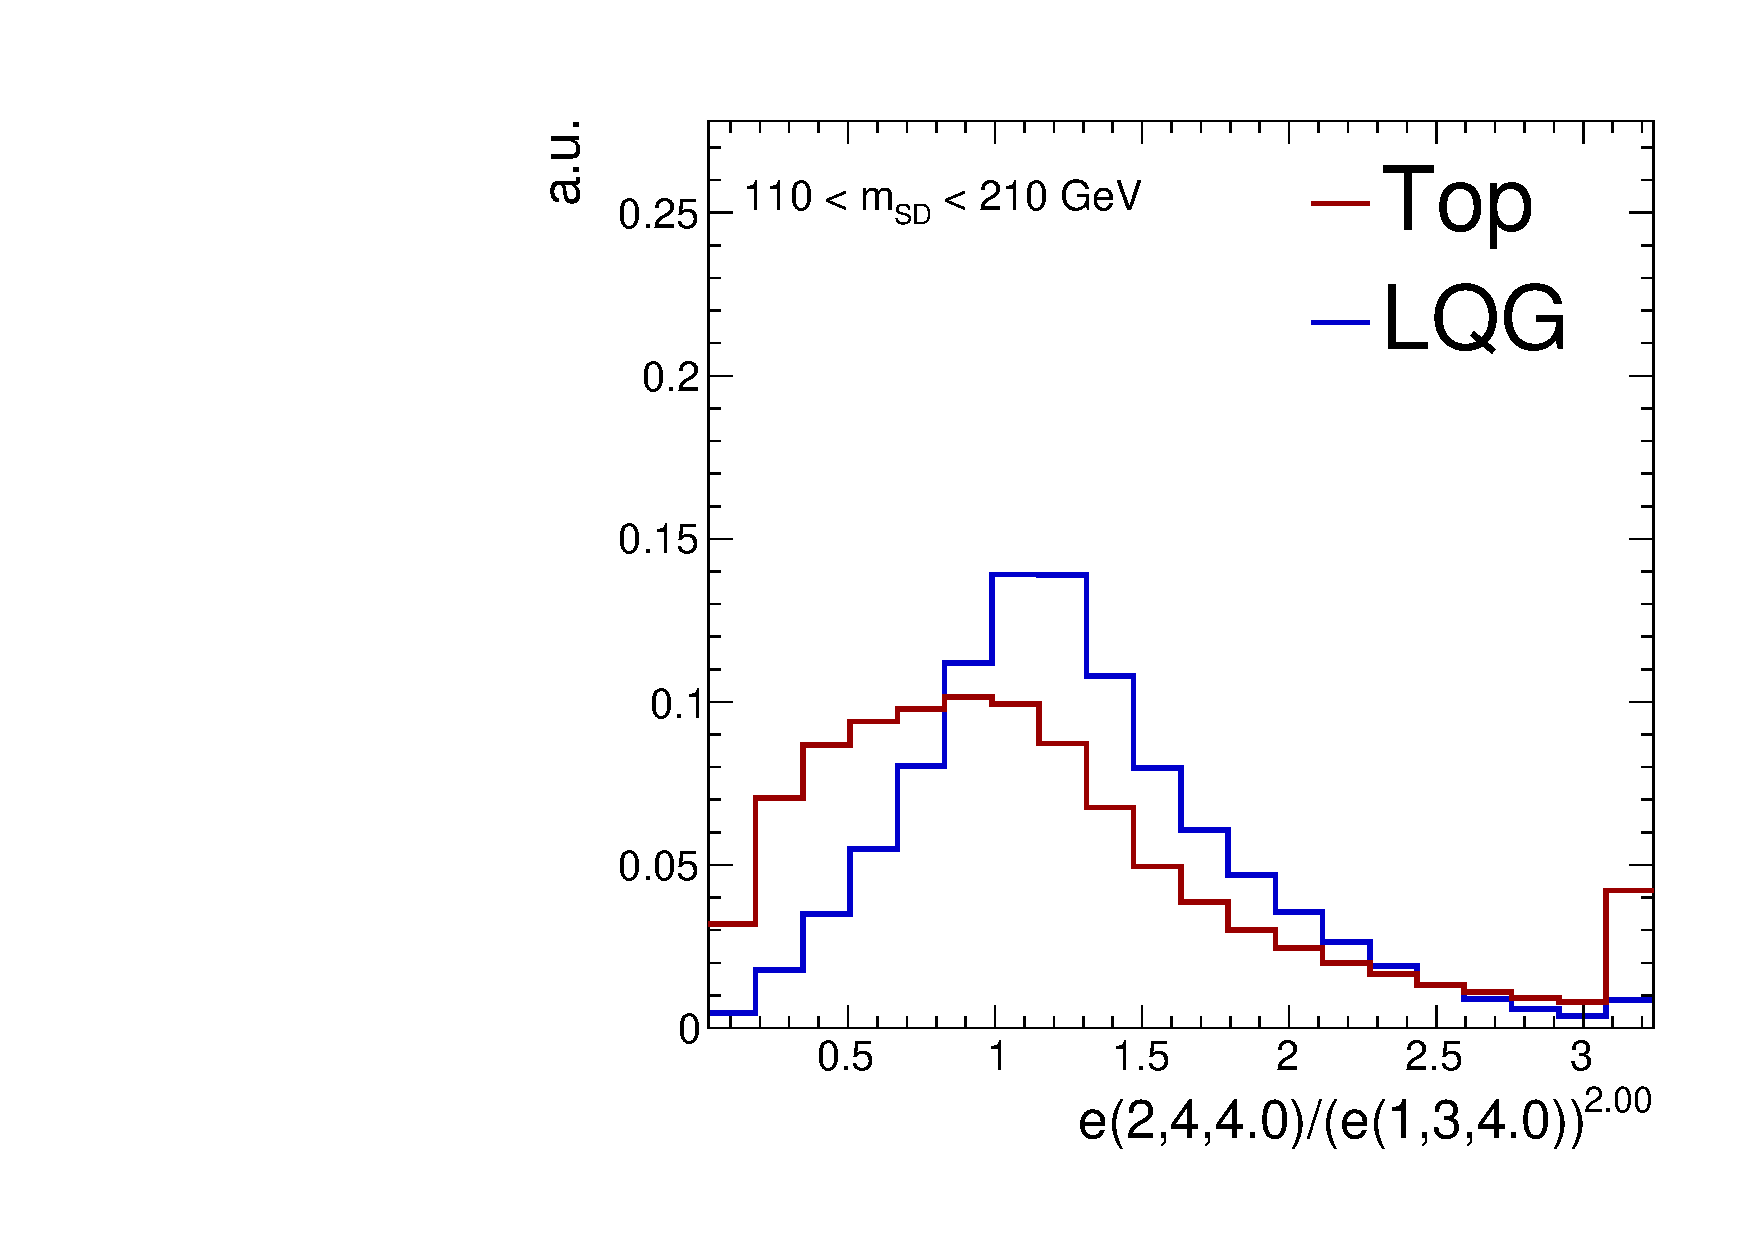
\includegraphics[width=\textwidth]{figures/toptagging/shapes/mass_ratio_24401340.pdf}
        \end{subfigure}
        \caption{Shape of the $N_3$ observables in top and LQG jets, for various values of $\beta$.}
        \label{fig:jets:n3}
    \end{center}
\end{figure}

While $N_3$ has a strong theoretical motivation, it is possible that other functions of ECFs  distinguish between top and LQG jets.
In order to construct observables that do not have a strong dependence on the jet \pt, we restrict ourselves to ratios of the form:
\begin{equation}
    \psi(a,N,\alpha,b,M,\beta) = 
    \frac{e(a,N,\alpha)}{\left(e(b,M,\beta)\right)^x} 
    \text{, where } M\leq N \text{ and } x = \frac{a\alpha}{b\beta}
\end{equation}
A large subset of this broader class of ECF observables are found to be useful (Figure~\ref{fig:jets:ecfrs}), including ratios not of the form $e(N=4)/e(N=3)$.

\begin{figure}[]
    \begin{center}
        \begin{subfigure}[t]{0.32\textwidth}
            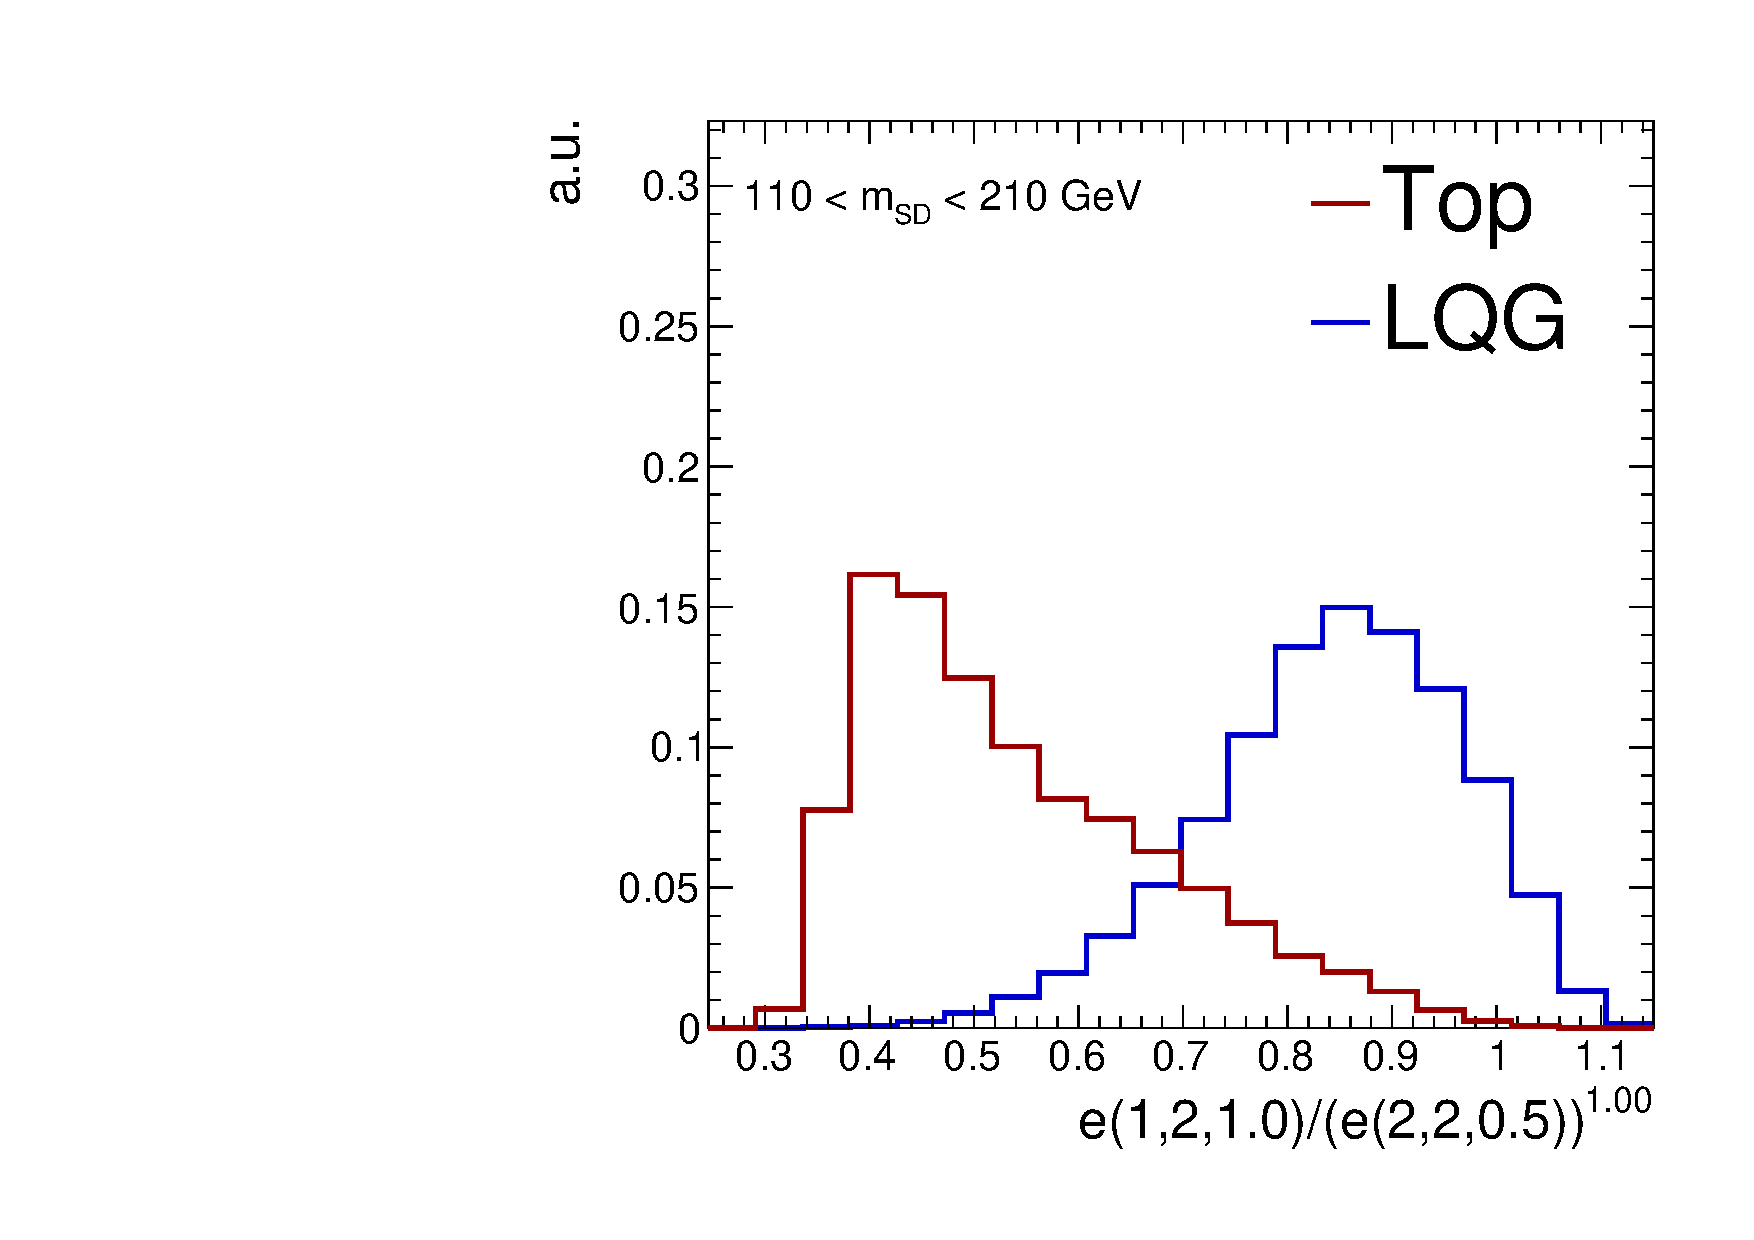
\includegraphics[width=\textwidth]{figures/toptagging/shapes/mass_ratio_12102205.pdf}
        \end{subfigure}
        \begin{subfigure}[t]{0.32\textwidth}
            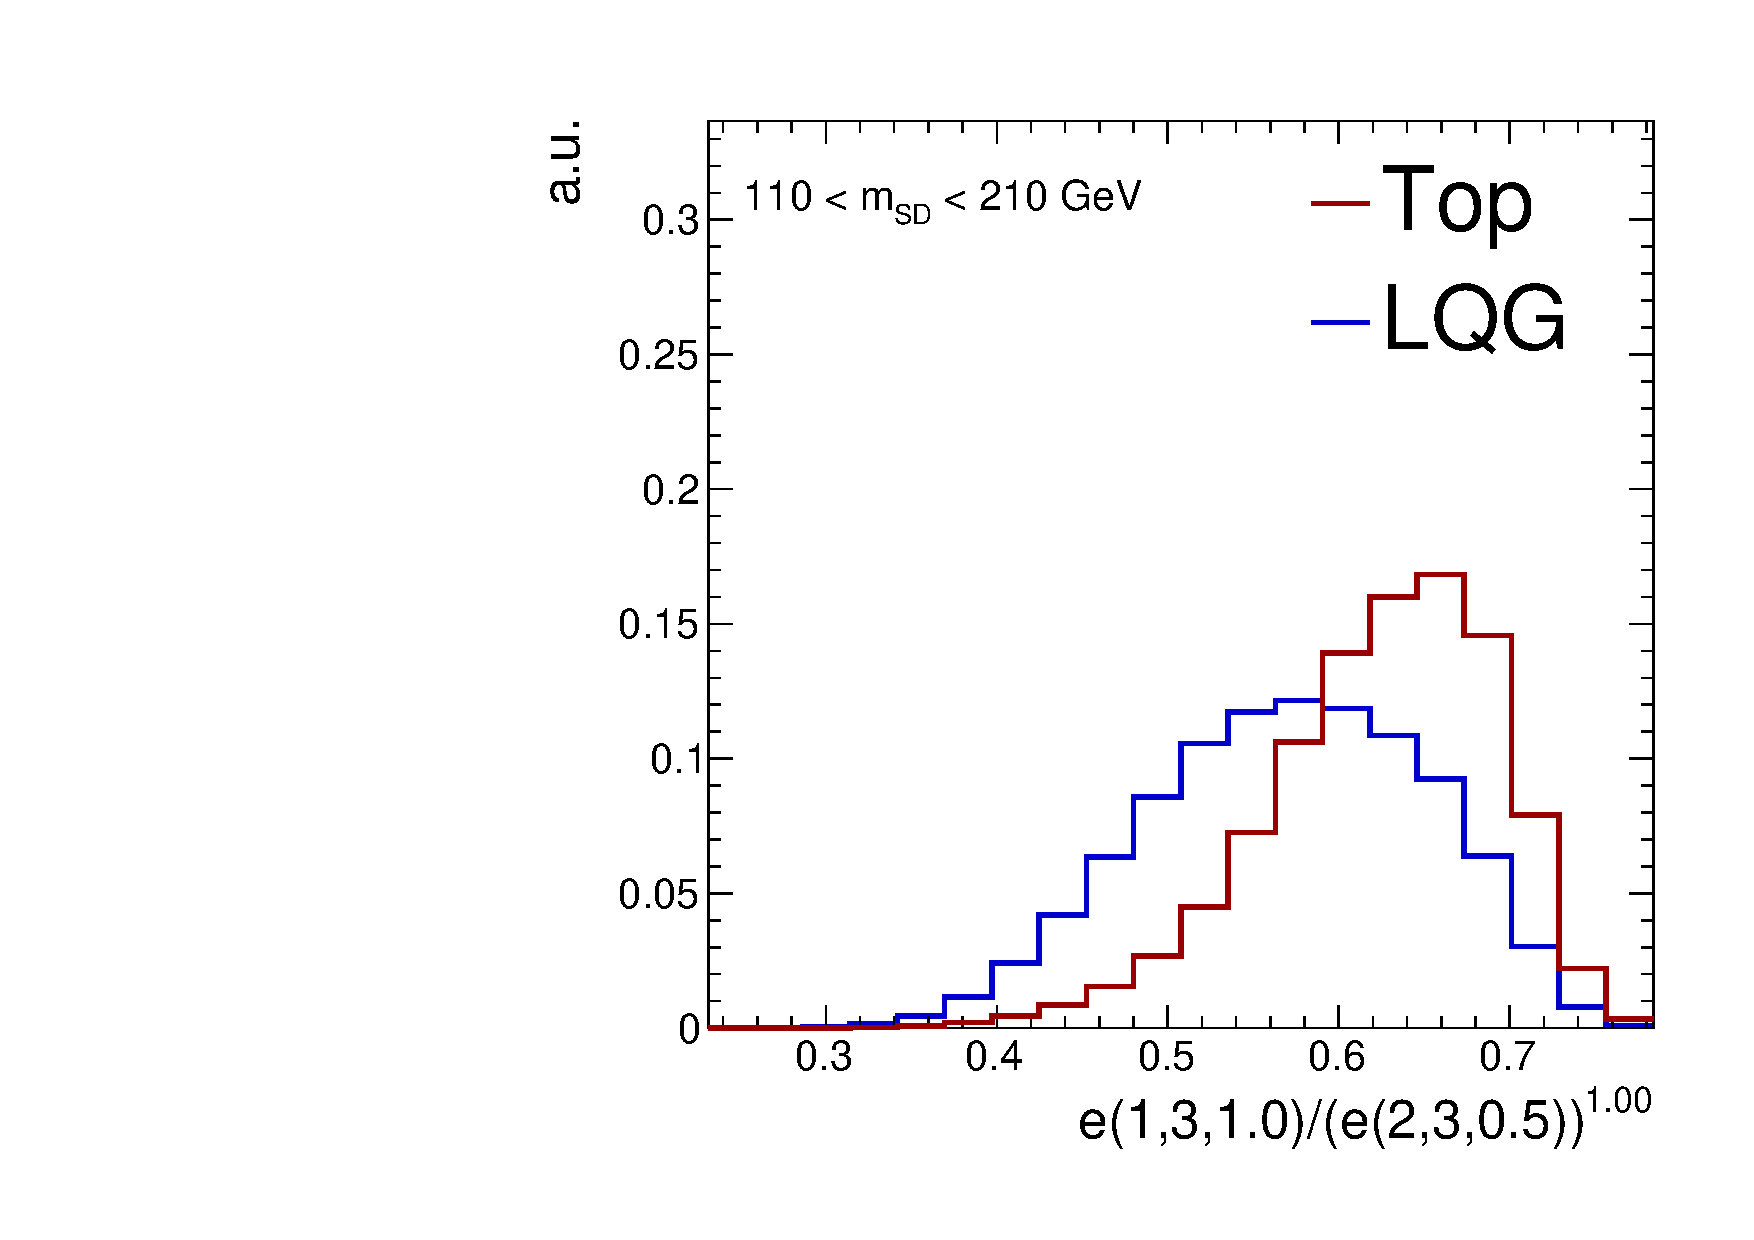
\includegraphics[width=\textwidth]{figures/toptagging/shapes/mass_ratio_13102305.pdf}
        \end{subfigure}
        \begin{subfigure}[t]{0.32\textwidth}
            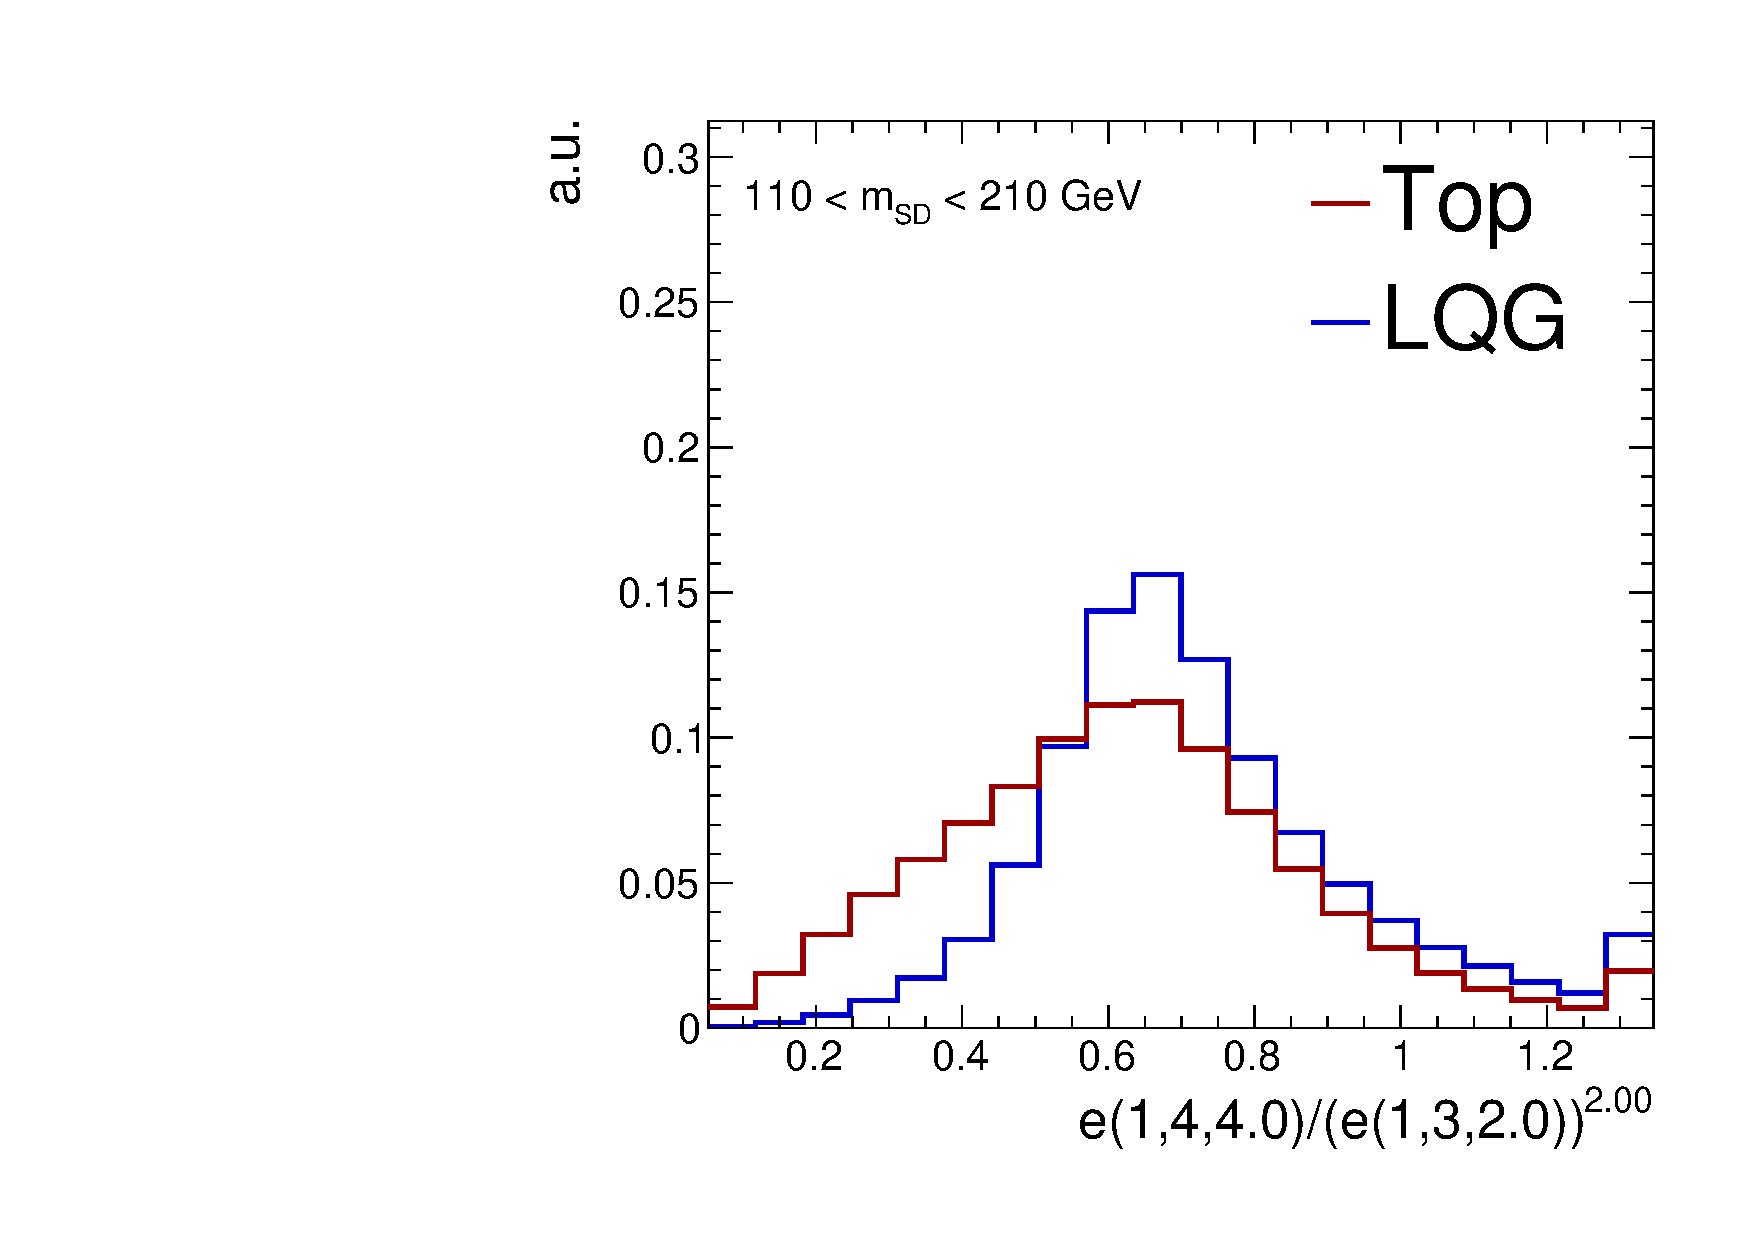
\includegraphics[width=\textwidth]{figures/toptagging/shapes/mass_ratio_14401320.pdf}
        \end{subfigure}
        \caption{Examples of non-trivial ECF ratios other than $N_3$ that separate top and LQG jet distributions.}
        \label{fig:jets:ecfrs}
    \end{center}
\end{figure}


\subsection{A combined tagger}
\label{sec:jets:bdt}

In principle, we have constructed an infinitely large space of jet substructure observables.
In practice, we only consider a finite sampling of ECF parameters:
\begin{gather}
    N \in \{1,2,3,4\} \nonumber \\ 
    o \in \{1,2,3\} \nonumber \\ 
    \beta \in \{0.5, 1, 2, 4\}
\end{gather}
This grid results in $\sim900$ $\psi$ observables.

\subsubsection{Boosted decision trees}
To build a single optimal observable out of all the $\{\psi_i\}$s, we will use a boosted decision tree (BDT).
A simplified algorithm to train a single decision tree node $n$ for classification is as follows:
\begin{enumerate}
    \item Choose a $\psi_j$, either by sampling randomly or selecting the one most optimal for the next step.
    \item Based on the training data fed to the node, select a decision boundary $d_n$ to optimize a loss function
          For classification, we use cross-entropy:
        \begin{gather}
            \ell(X,y;j,d_n) =  -\hat\pi_B\ln\hat\pi_B -\hat\pi_S\ln\hat\pi_S \\ 
            \hat\pi_c = P(y=c | \psi_j < d_n) 
        \end{gather}
\end{enumerate}
A tree is built iteratively:
\begin{enumerate}
    \item Train a node $n$ using the above criteria. 
    \item If a stopping condition is not met, train one node on the samples that pass $n$ and another on the samples that fail.
          Stopping conditions can take into account features including:
    \begin{itemize}
            \item Number of nodes
            \item Depth of tree
            \item Relative change in $\ell(n)$
    \end{itemize}
\end{enumerate}
Figure~\ref{fig:jets:dt} provides a pictorial example of how a decision tree can be built. 

\begin{figure}[]
    \begin{center}
        \begin{subfigure}[t]{0.32\textwidth}
            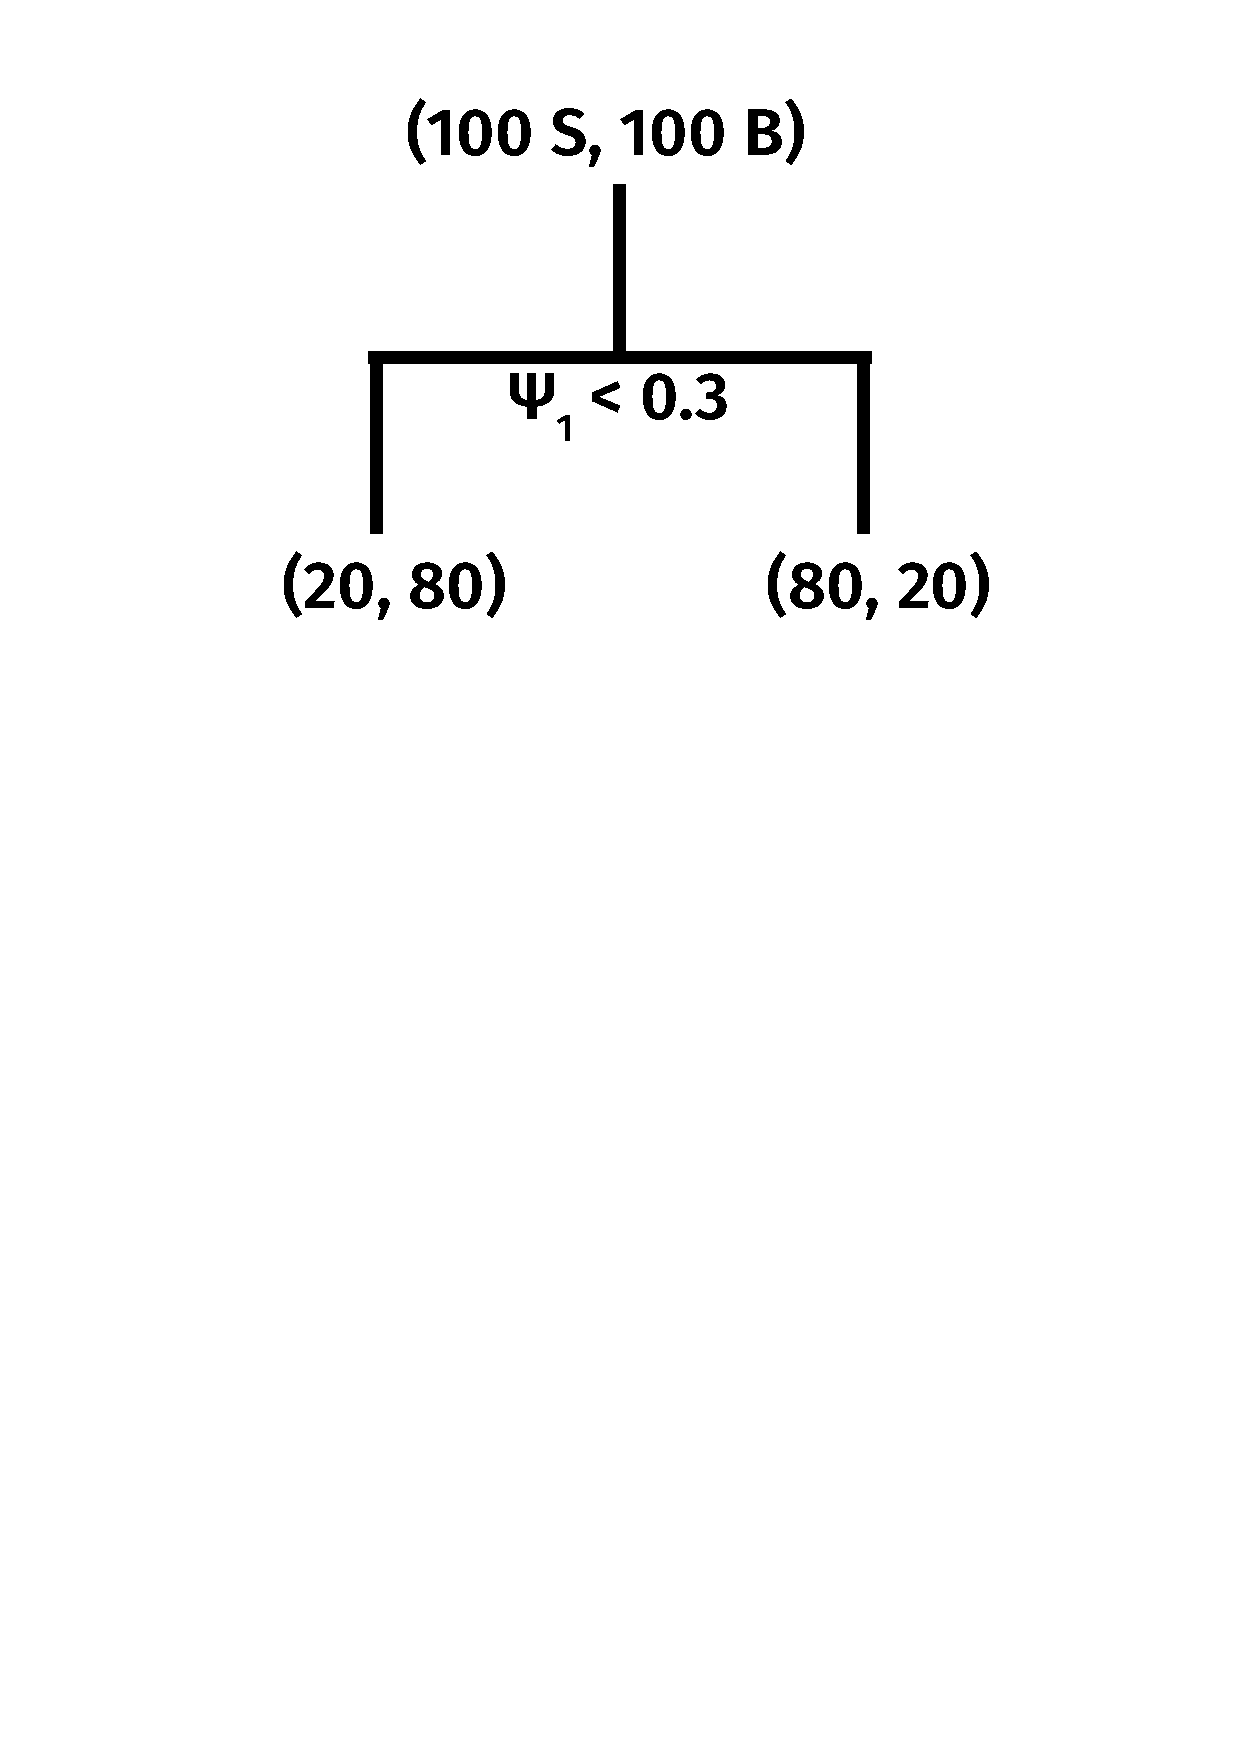
\includegraphics[width=\textwidth]{figures/toptagging/bdt/tree0.pdf}
            \caption{}
        \end{subfigure}
        \begin{subfigure}[t]{0.32\textwidth}
            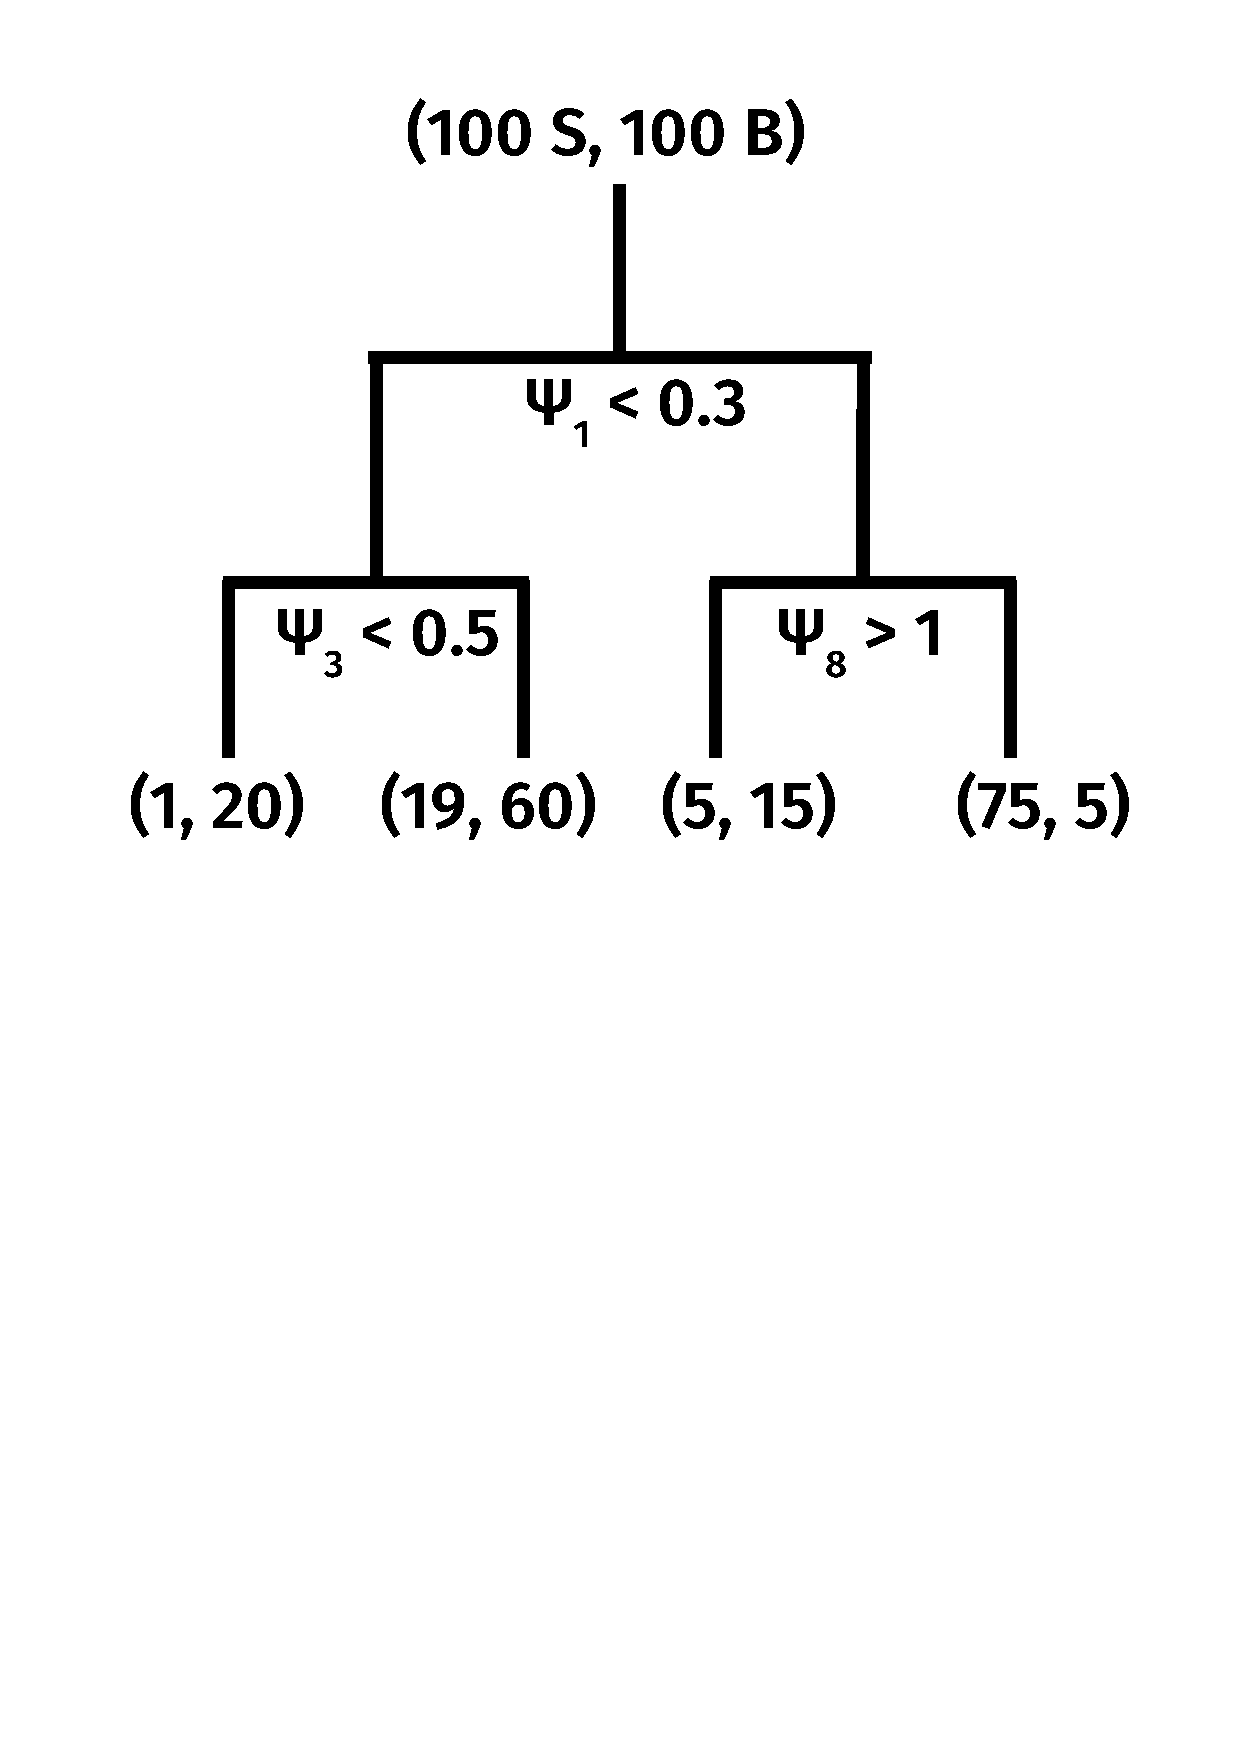
\includegraphics[width=\textwidth]{figures/toptagging/bdt/tree1.pdf}
            \caption{}
        \end{subfigure}
        \begin{subfigure}[t]{0.32\textwidth}
            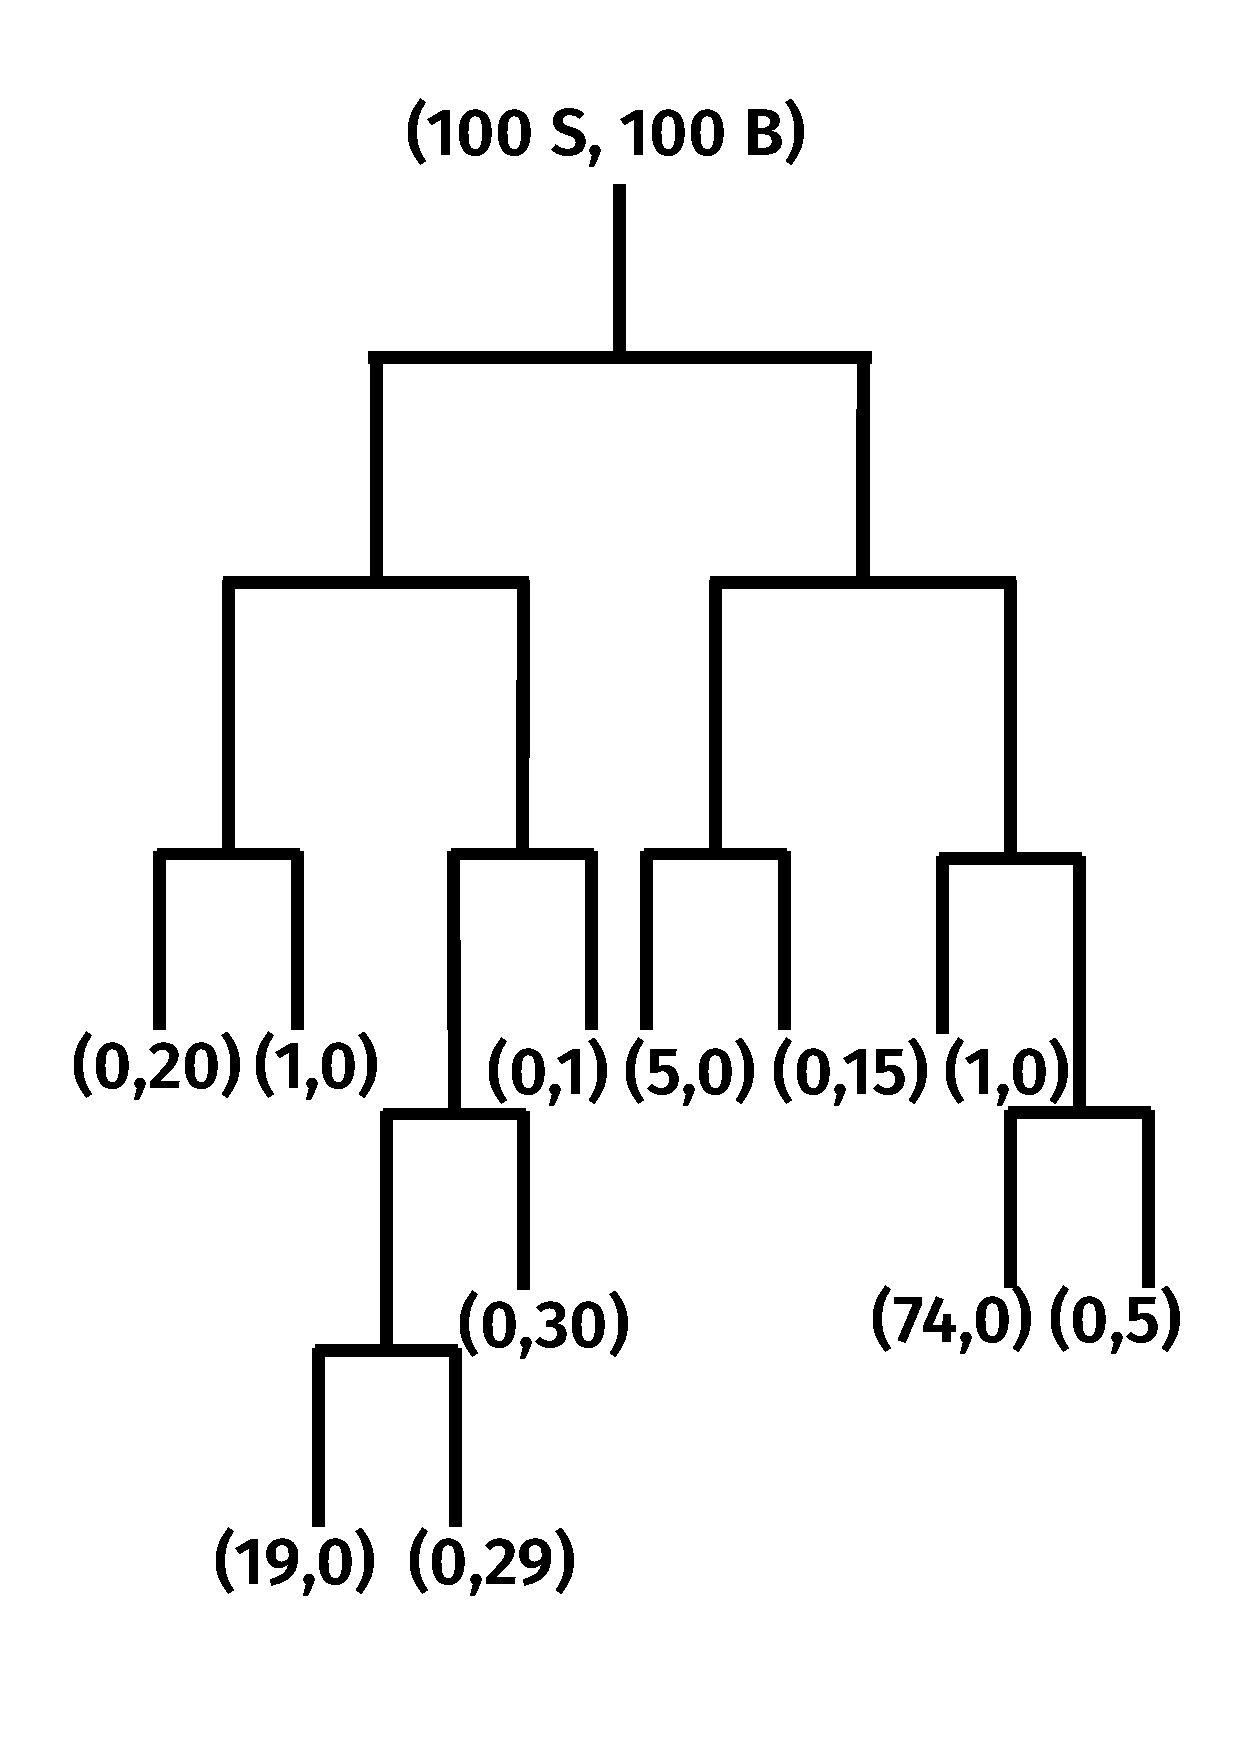
\includegraphics[width=\textwidth]{figures/toptagging/bdt/tree2.pdf}
            \caption{}
        \end{subfigure}
        \caption{Steps in greedily training a simple decision tree.
                 At each node, the number of signal and background samples is indicated by the tuple $(S,B)$.
                 For example, the root node in step (a) is fed 100 signal and 100 background samples.
                 The learning rule decides the optimal decision at this node is $\psi_i < 0.3$, which subdivides the 200 samples into two subsamples with composition $(20,80)$ and $(80,20)$.
                 Step (b) shows a further partitioning of the training samples using additional features.
                 Step (c) shows a fully trained tree, in which each leaf node only contains signal or background samples.
                 Such a tree cannot be further refined, but earlier stopping conditions may also be used.}
        \label{fig:jets:dt}
    \end{center}
\end{figure}

Decision trees can very accurately describe training data, but they also pathologically overfit the data.
\emph{Boosting} many shallow trees is a standard method to mitigate this and retain descriptive power.
The simplicity of individual trees prevents overfitting, while boosting many trees allows for a complex model.
The result of a BDT is a classifier $f_n(x) = \sum_{i=0}^n \nu^i T_i(x)$, where $\nu\leq 1$ is tunable and each $T_i$ is a decision tree. 
Each $T_j$ is trained to correct for the residual error from the previously trained trees $f_j(x) =  \sum_{i=0}^j \nu^i T_i(x)$
A simplified algorithm to train a BDT is as follows:
\begin{enumerate}
    \item Define a global loss function, e.g.:
        \begin{equation} L(y_i; f_i) = \ln\left(1 + \exp(-y_if_i)\right)\end{equation}
    \item Train a single tree $T_0$ and initialize classifier $f_0 = T_0$
    \item Until some stopping condition (index $m=1,\dots,n$):
    \begin{enumerate}
      \item[3.1.] Compute the \emph{residual} as the gradient of the global loss with respect to the classifier $f_{m-1}$:
        \begin{equation}r_{mi} = -\nabla_f L(y_i; f) |_{f=f_{m-1}(\bm\psi_i)}\end{equation}
      \item[3.2.] Fit a regression tree $T_m$ to predict $r_{mi}$ as a function of $x_i$:
        \begin{equation}\ell(X,r_m;j,d,\hat{r}) = \sum_{i | \psi_{ji} < d} (r_{mi} - \hat r)^2\end{equation}
      \item[3.3.] Update $f_m = f_{m-1} + \nu T_m$
    \end{enumerate}
\end{enumerate}

The decision tree training and boosting algorithms we use are provided by the Toolkit for Multivariate Analysis~\cite{tmva}.

\subsubsection{Training the BDT}

While we would like to train a BDT on the entire space of $\{\psi\}$, there are two issues to be solved: poorly modeled ratios and a large feature space.
Firstly, the descriptions of many ECF ratios in LQG jets are poorly-simulated by MC (Figure~\ref{fig:jets:datamc_ratios}).
More systematically, we can compute the CDF of each $\psi$ and define a score: 
\begin{equation}
    -\log_{10} \mathrm{KS}(F_\mathrm{data}(\psi_i), F_\mathrm{MC}(\psi_i)) = -\log_{10} \max \left|F_\mathrm{data}(\psi_i) - F_\mathrm{MC}(\psi_i)\right|
\end{equation}
where $F$ represents the CDF and $\mathrm{KS}$ denotes the Kolmogorov-Smirnov metric on probability distributions.
The score is close to 0 for poorly-simulated distributions and approaches $\infty$ as $F_\mathrm{MC} \rightarrow F_\mathrm{data}$..
Figure~\ref{fig:jets:ks} parameterizes this as a function of $N/M$ (ratio of the number of particles) and $a\alpha/b\beta$ (ratio of the angular powers) and shows an interesting structure.
It is found that $3/2$ and $4/2$ ratios are uniformly poorly modeled, as are ratios with large $a\alpha/b\beta$. 
In what follows, we only consider ECF ratios with $-\log_{10}\mathrm{KS} > 1$, which corresponds to the bottom-left of Figure`\ref{fig:jets:ks}. 

\begin{figure}[]
    \begin{center}
        \begin{subfigure}[t]{0.32\textwidth}
            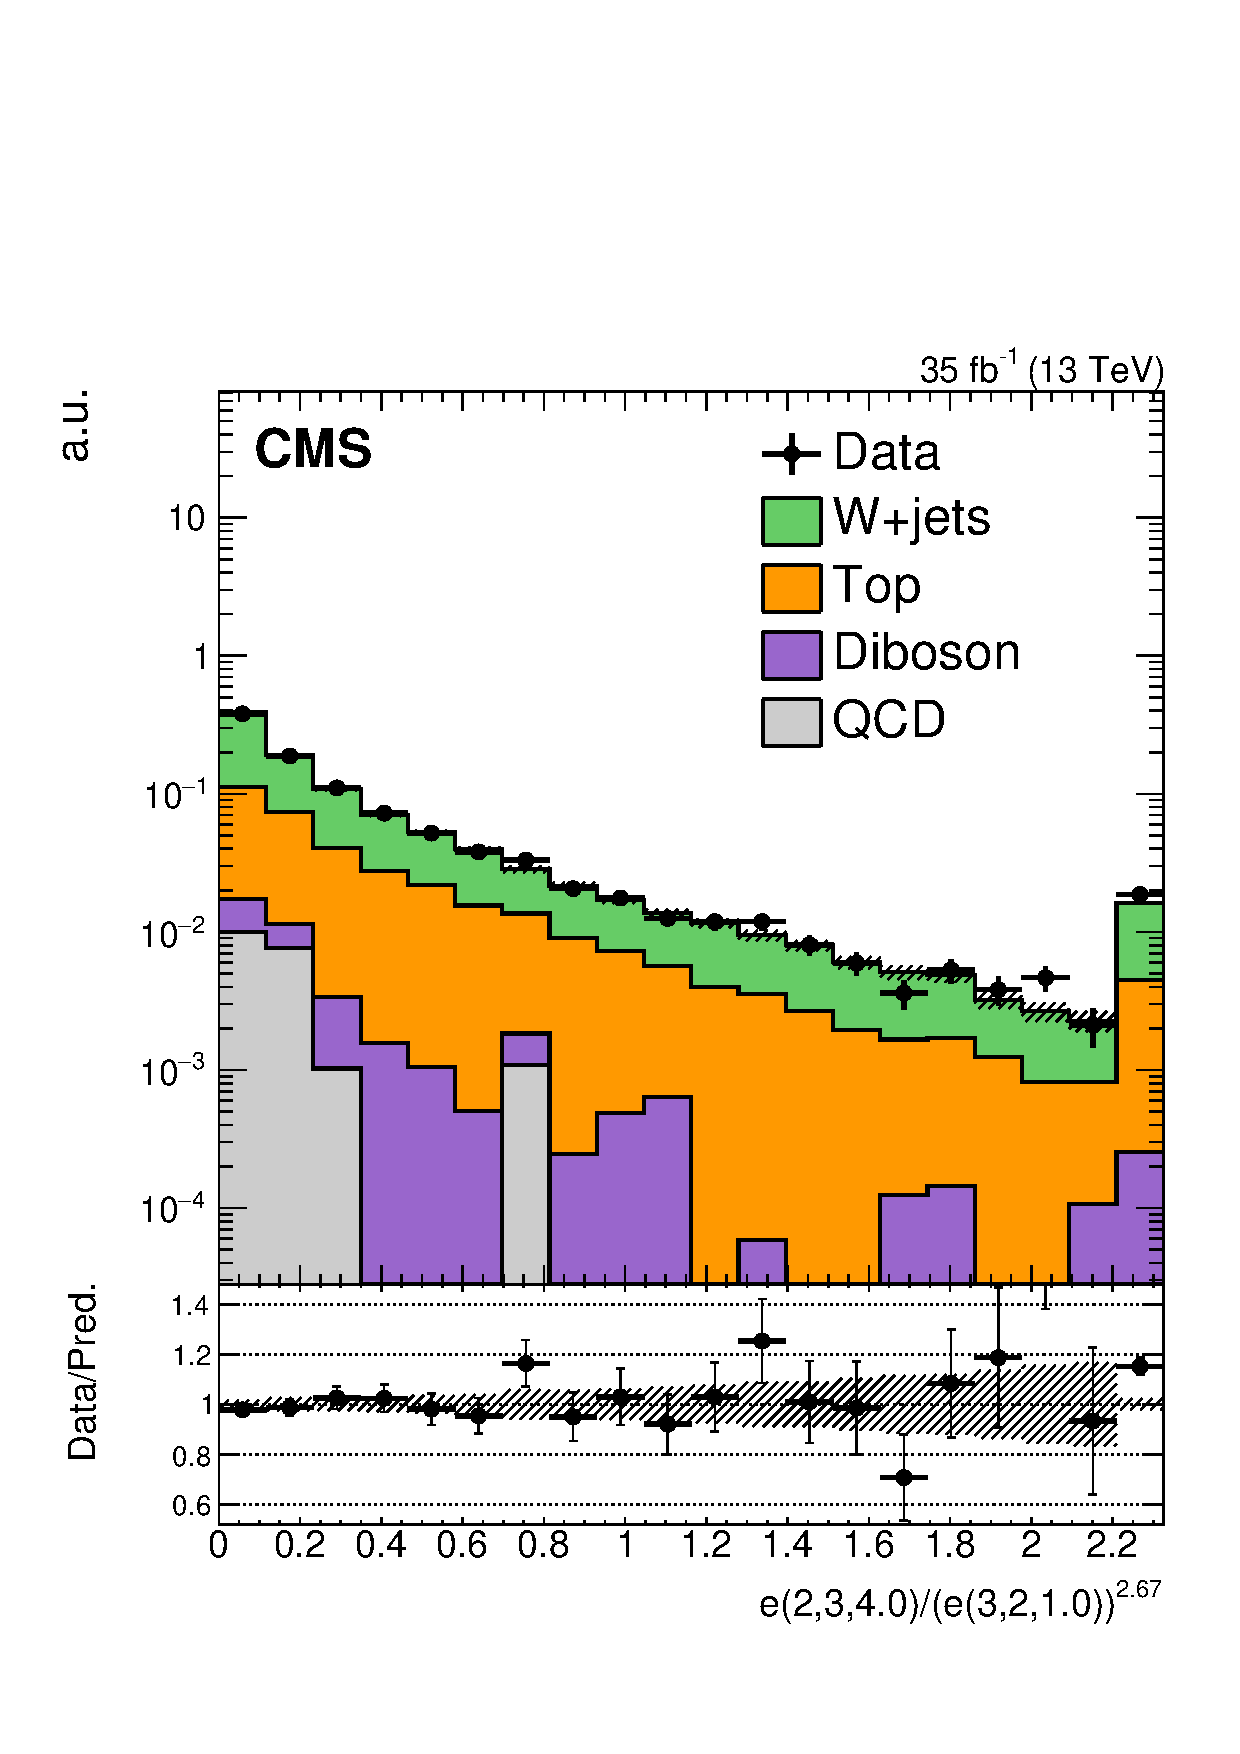
\includegraphics[width=\textwidth]{figures/toptagging/datamc/singlemuonw_ratio_23403210_logy.pdf}
        \end{subfigure}
        \begin{subfigure}[t]{0.32\textwidth}
            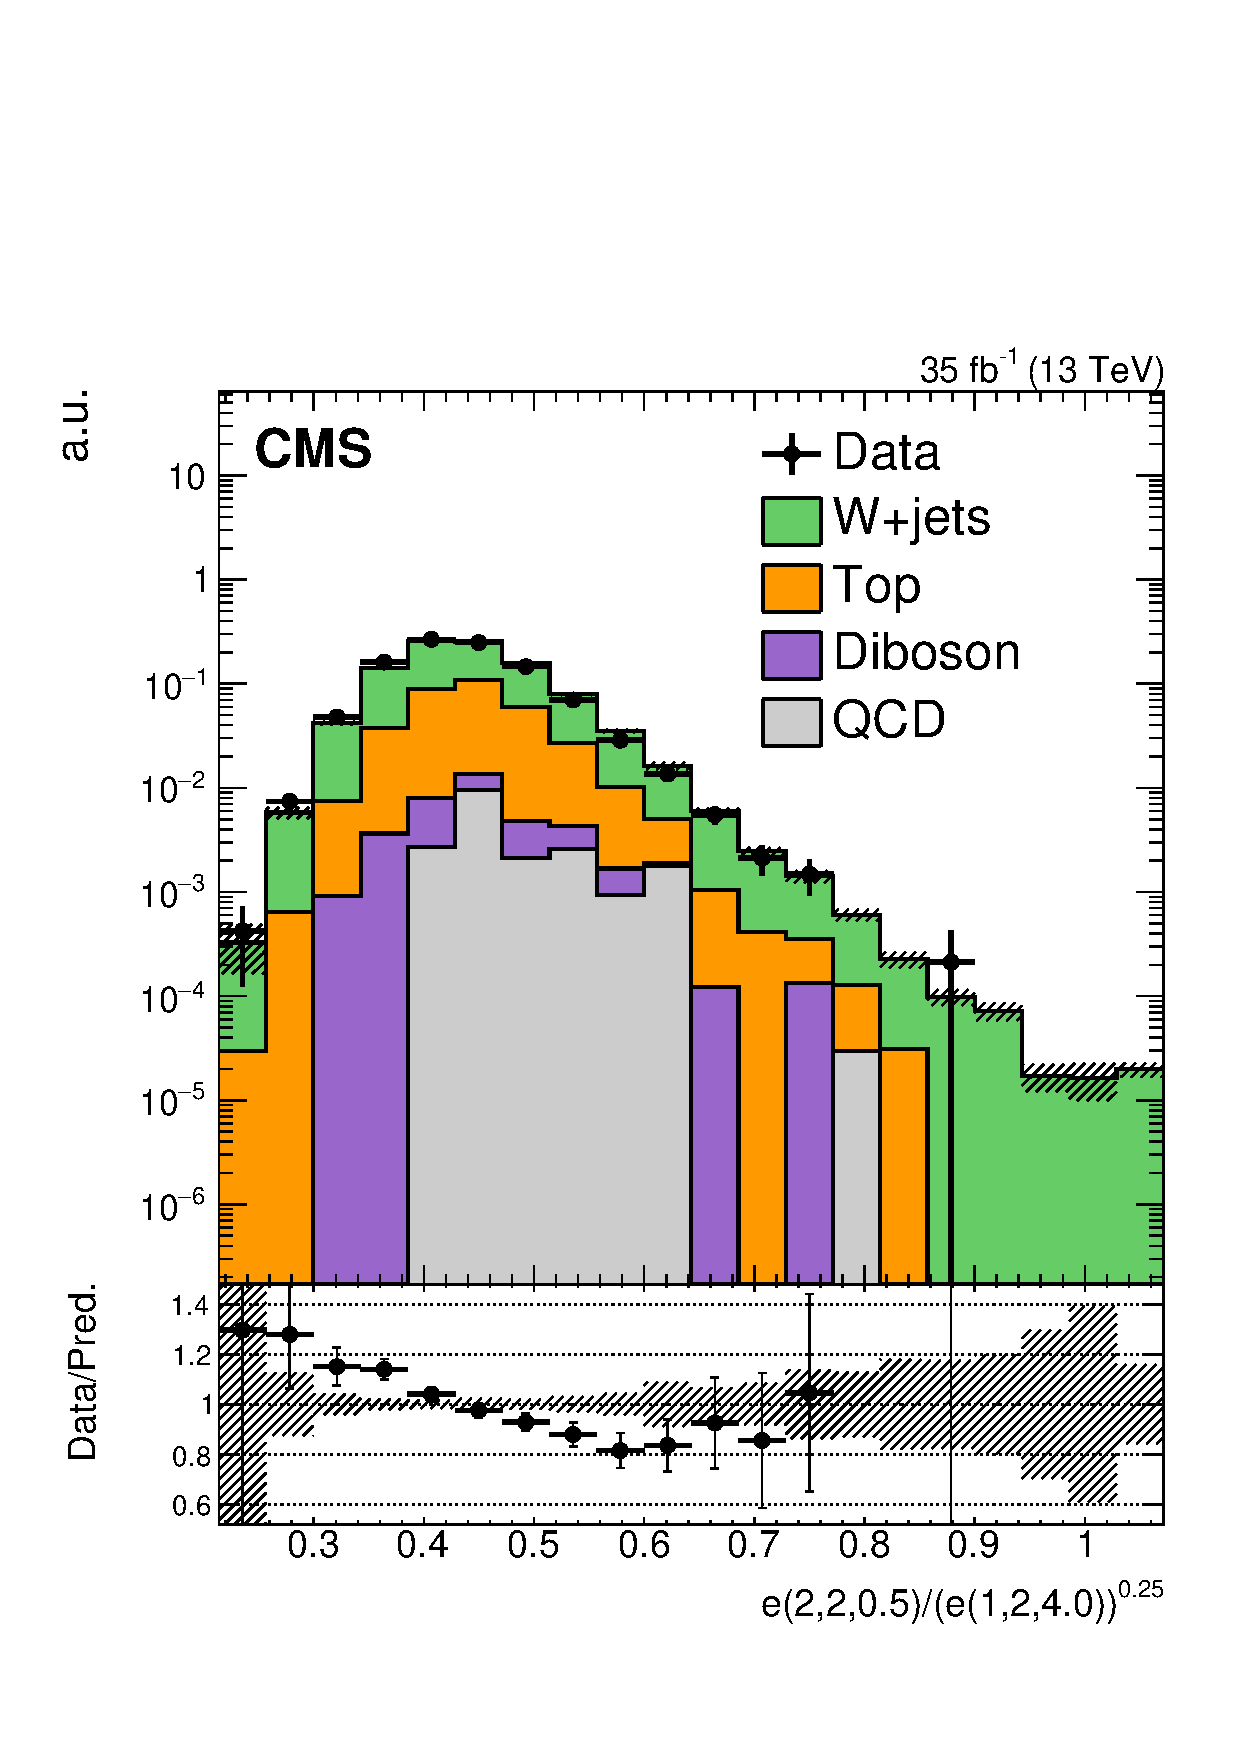
\includegraphics[width=\textwidth]{figures/toptagging/datamc/singlemuonw_ratio_22051240_logy.pdf}
        \end{subfigure}
        \caption{Two different ECF ratios in a $W$+jets selection, heavily enriched in LQG jets.
                 One is fairly well-modeled, while the other is not. }
        \label{fig:jets:datamc_ratios}
    \end{center}
\end{figure}

\begin{figure}[]
    \begin{center}
        \begin{subfigure}[t]{0.4\textwidth}
            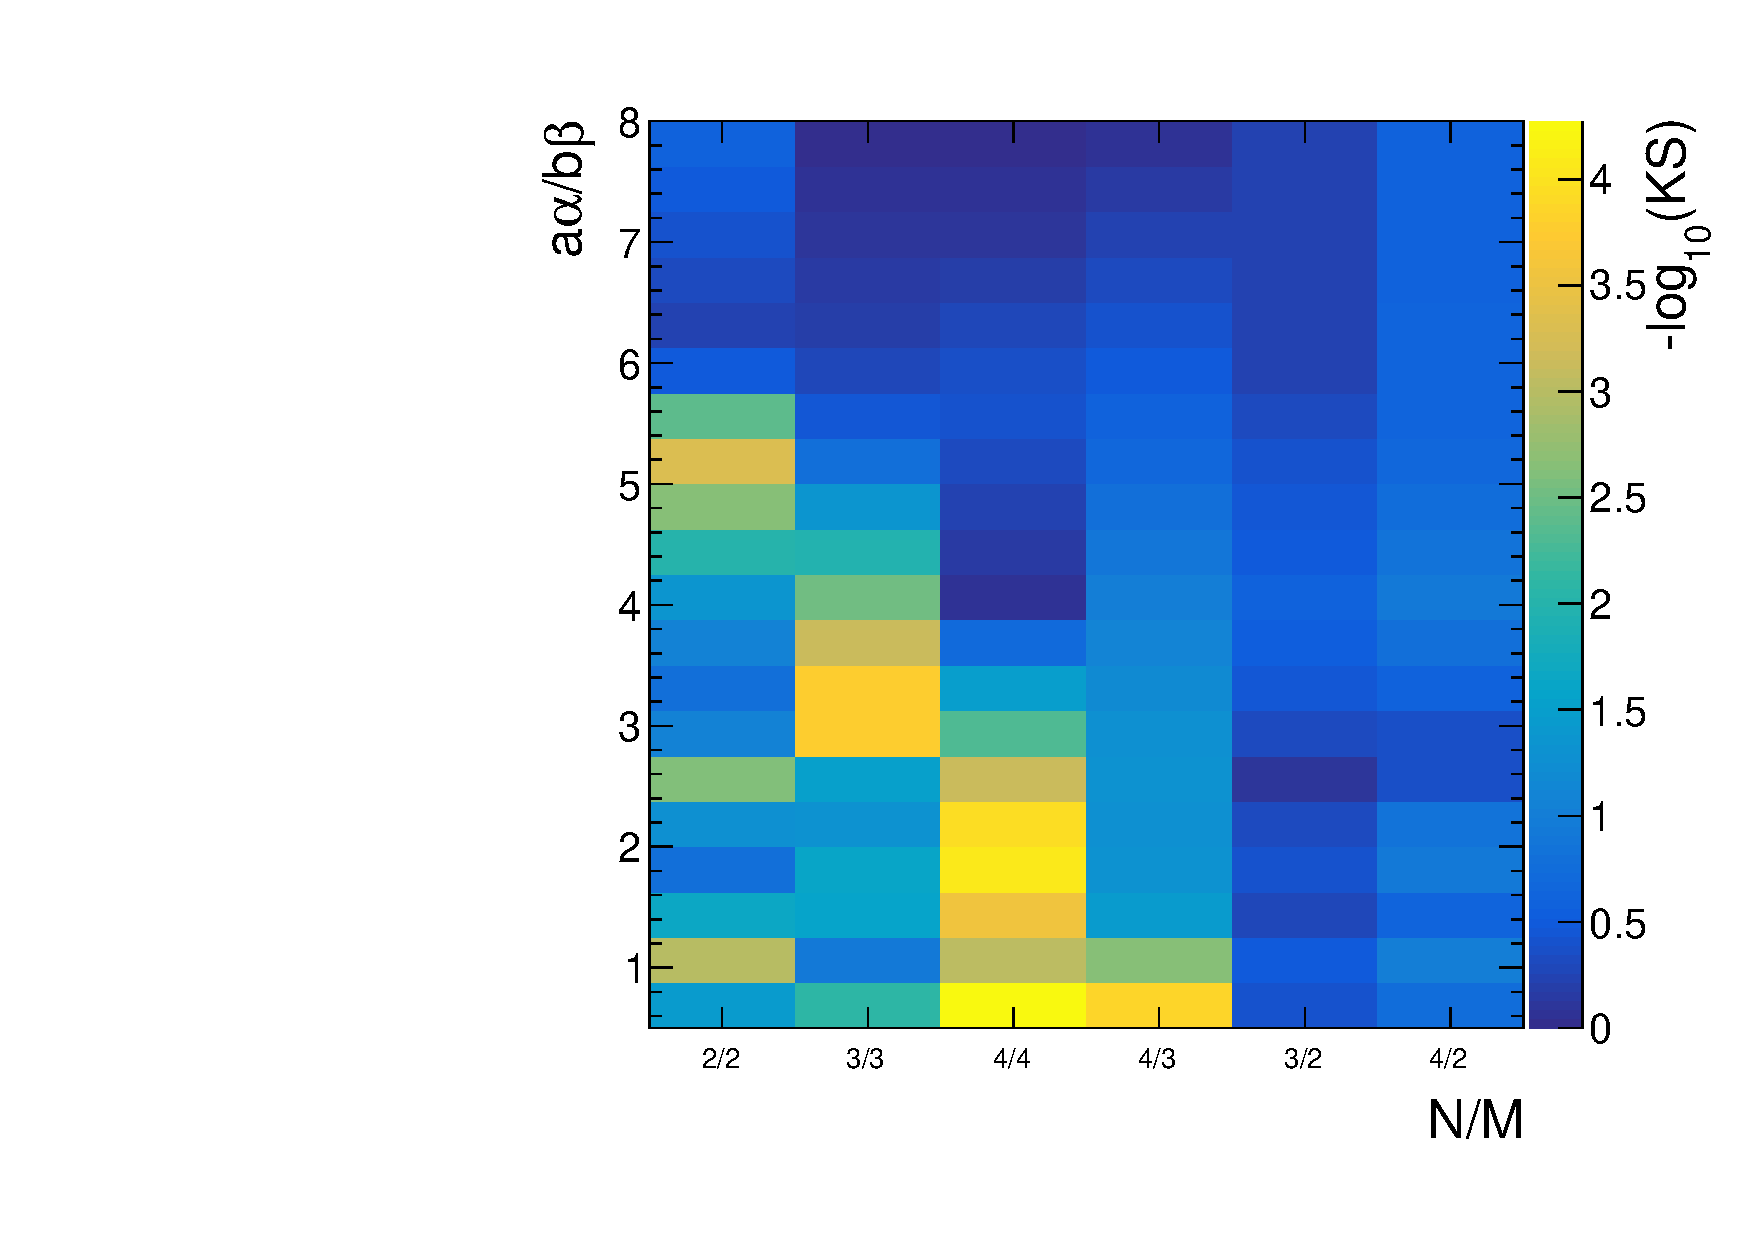
\includegraphics[width=\textwidth]{figures/toptagging/datamc/scanmnab.pdf}
        \end{subfigure}
        \caption{The $-\log_{10}\mathrm{KS}$ metric as a function of $N/M$ and $a\alpha/b\beta$, computed using events enriched in LQG jets. }
        \label{fig:jets:ks}
    \end{center}
\end{figure}

Even after filtering poorly-modeled ratios, we are left with a sampled $\psi$ grid of ${\sim400}$ points.
It is desirable to reduce the size of the feature space, as computing each ECF is somewhat computationally-intensive: an $N$-point ECF on a $p$-particle jet has $\binom{N}{p}$ terms. 
Note that standard pre-processing techniques, like principal component analysis, do not reduce the number of features to be computed. 
Methods like L1 regularization~\cite{nns} do force sparsity in the feature space, but cannot be trivially applied to BDTs. 
Therefore, we introduce a targeted iterative training method to solve this problem:
\begin{enumerate}
    \item Train a BDT with trees $T_1,\dots,T_n$
    \item For each $\psi_i$, define a score:
        \begin{equation}
             s_i = \sum_{m=1}^n \nu^{m-1} \sum_{\text{nodes using $\psi_i$ in $T_m$}} N_\text{samples}(\mathrm{node}) \times \left(\ell(\mathrm{node}) - \ell(\mathrm{parent})\right)^2  
        \end{equation}
    \item Remove one or more $\psi_i$ with smallest $s_i$ and repeat. 
\end{enumerate}
Iterative training is expensive and can require the training of $\mathcal{O}(50)$ BDTs.
It is semi-parallelizable, and the entire process typically takes a few hours.
However, as the inference samples are 1-2 orders of magnitude larger than the training samples, this method reduces the total CPU time needed to run an analysis. 
Figure~\ref{fig:jets:training} shows background acceptance rate at $\epsilon_\mathrm{sig}=0.5$ (a proxy for the global loss) as a function of feature space size. 
For illustrative purposes, we only show the range $[1,50]$.
The inputs for this training are the ECF ratios, as well as $\tau_{32}^\SD$ and $\frec$, which provide additional information.

\begin{figure}[]
    \begin{center}
        \begin{subfigure}[t]{0.5\textwidth}
            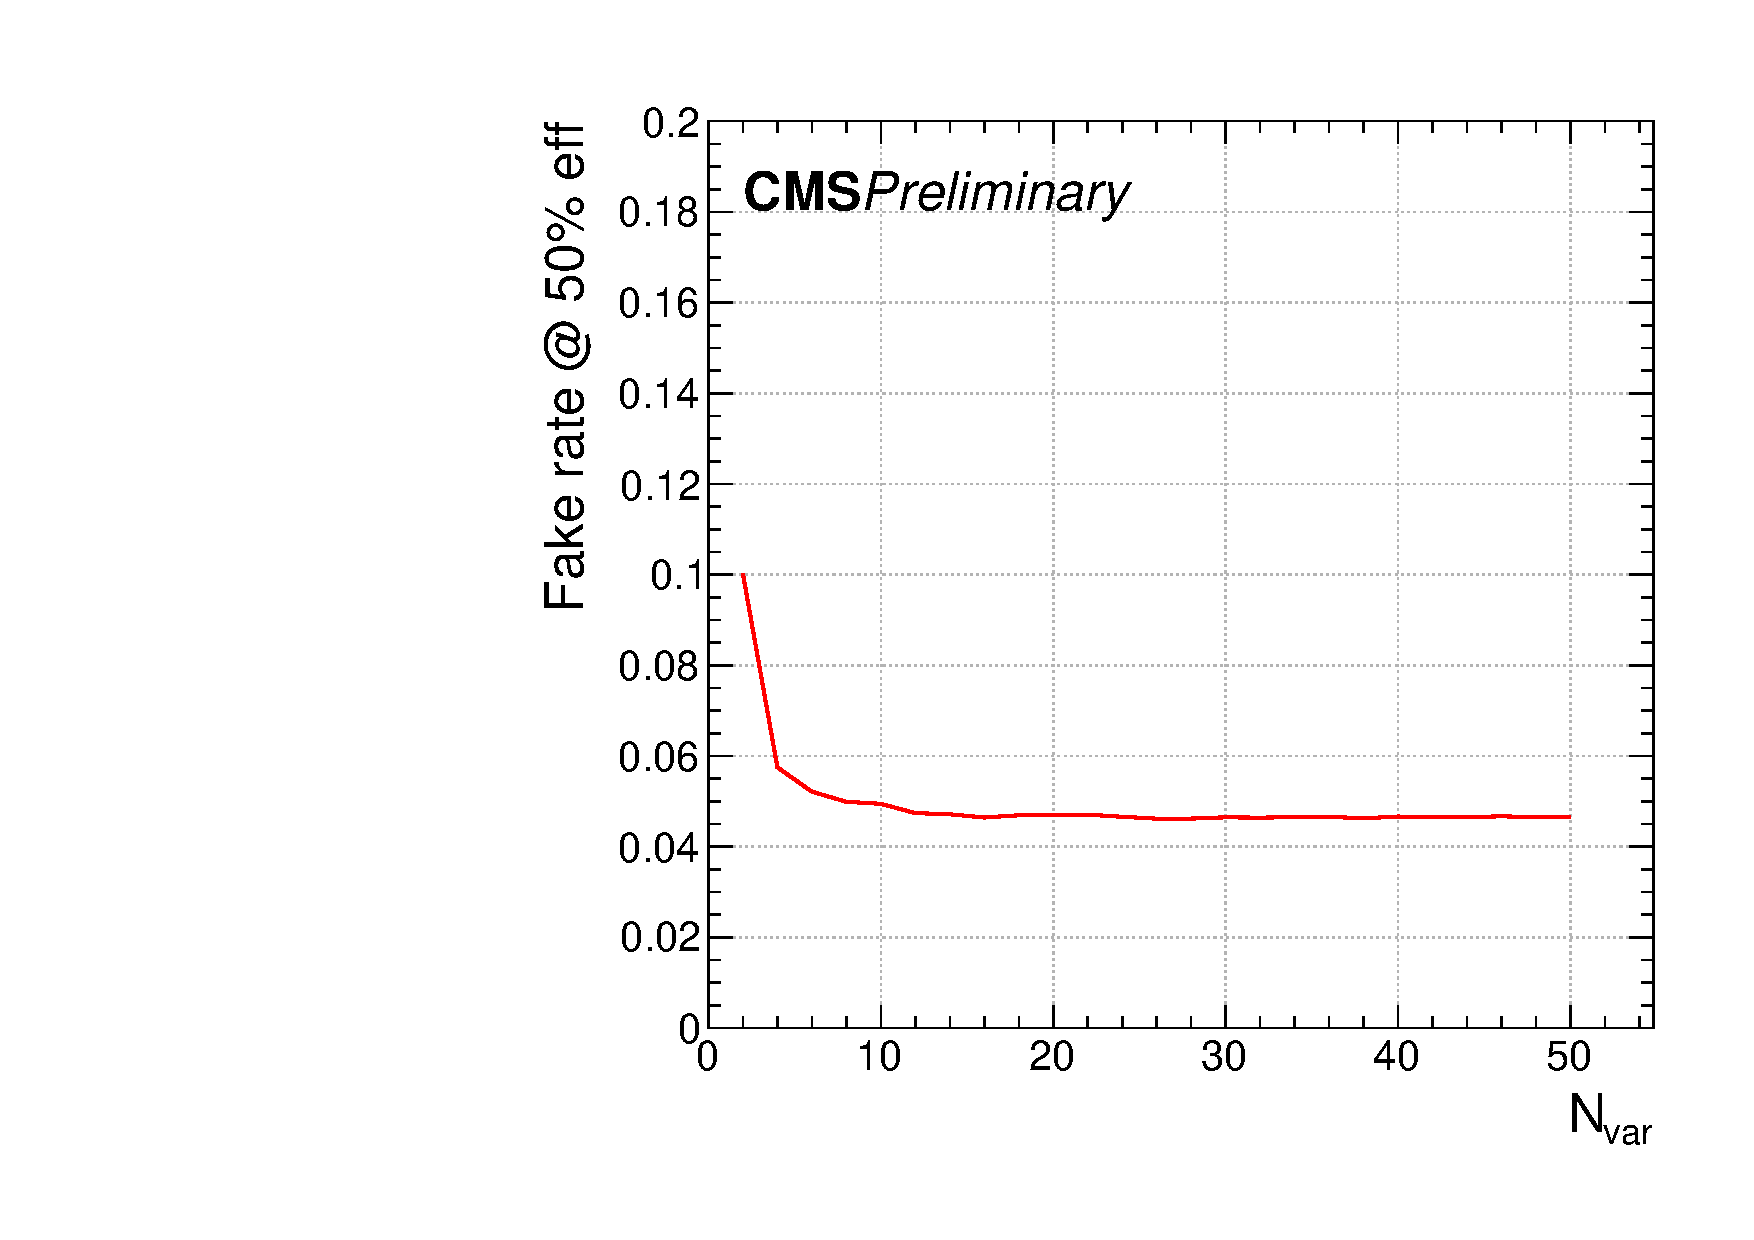
\includegraphics[width=\textwidth]{figures/toptagging/bdt/fakerate_vs_eff50.pdf}
        \end{subfigure}
        \caption{Performance of BDTs as a function of the number features used in the training.
                 The performance is defined by the fraction of LQG jets accepted by the BDT when the signal efficiency is fixed at $50\%$.}
        \label{fig:jets:training}
    \end{center}
\end{figure}

The background acceptance reaches a minumum with 13 features, and so we choose this configuration as the final BDT.
The features are:
\begin{gather}
    \frac{e(1,4,20)}{e(1,3,10)^2},~
    \frac{e(1,4,40)}{e(1,3,20)^2},~
    \frac{e(2,4,05)}{e(1,3,05)^2},~
    \frac{e(2,4,10)}{e(1,3,10)^2},~
    \frac{e(2,4,10)}{e(2,3,05)^2},~
    \frac{e(2,4,20)}{e(1,3,20)^2} \nonumber \\ 
    \frac{e(1,2,20)}{e(1,2,10)^2},~
    \frac{e(1,3,40)}{e(2,3,20)},~
    \frac{e(3,3,10)}{e(1,3,40)^{3/4}},~
    \frac{e(3,3,10)}{e(2,3,20)^{3/4}},~
    \frac{e(3,3,20)}{e(3,3,40)^{1/2}}\nonumber \\ 
    \tau_{32}^\SD,~ \frec 
    \label{eq:jets:features}
\end{gather}
While a number of $N_3$ or other $4/3$ ratios appear in this list, we find a number of $2/2$ and $3/3$ ratios to contribute meaningfully to the classification task as well. 
Figure~\ref{fig:jets:features} shows the distributions of all selected features. 
Figure~\ref{fig:jets:roc} shows the background acceptance as a function of signal efficiency, comparing the final BDT (``Combined BDT'') to several other taggers.
The standard LHC tagger prior to this work is $\tau_{32}^\SD$, which, by itself, has a worse performance than the BDTs.
The Combined BDT's performance is near that of a BDT trained with many ECFs, including poorly modeled ones (``50 ECF'').
Removing $\tau_{32}^\SD$ and $\frec$ from Equation~\ref{eq:jets:features} results in the ``11 ECF'' BDT.
Therefore, the addition of these two features is critical to reaching the maximal performance achievable with the ECF ratio set, if description in simulation were not a concern.
At fixed signal efficiency $\epsilon_\mathrm{sig} = 0.5$, the combined BDT reduces the background acceptance by 30\% relative to $\tau_{32}^\SD$. 

\begin{figure}[]
    \begin{center}
        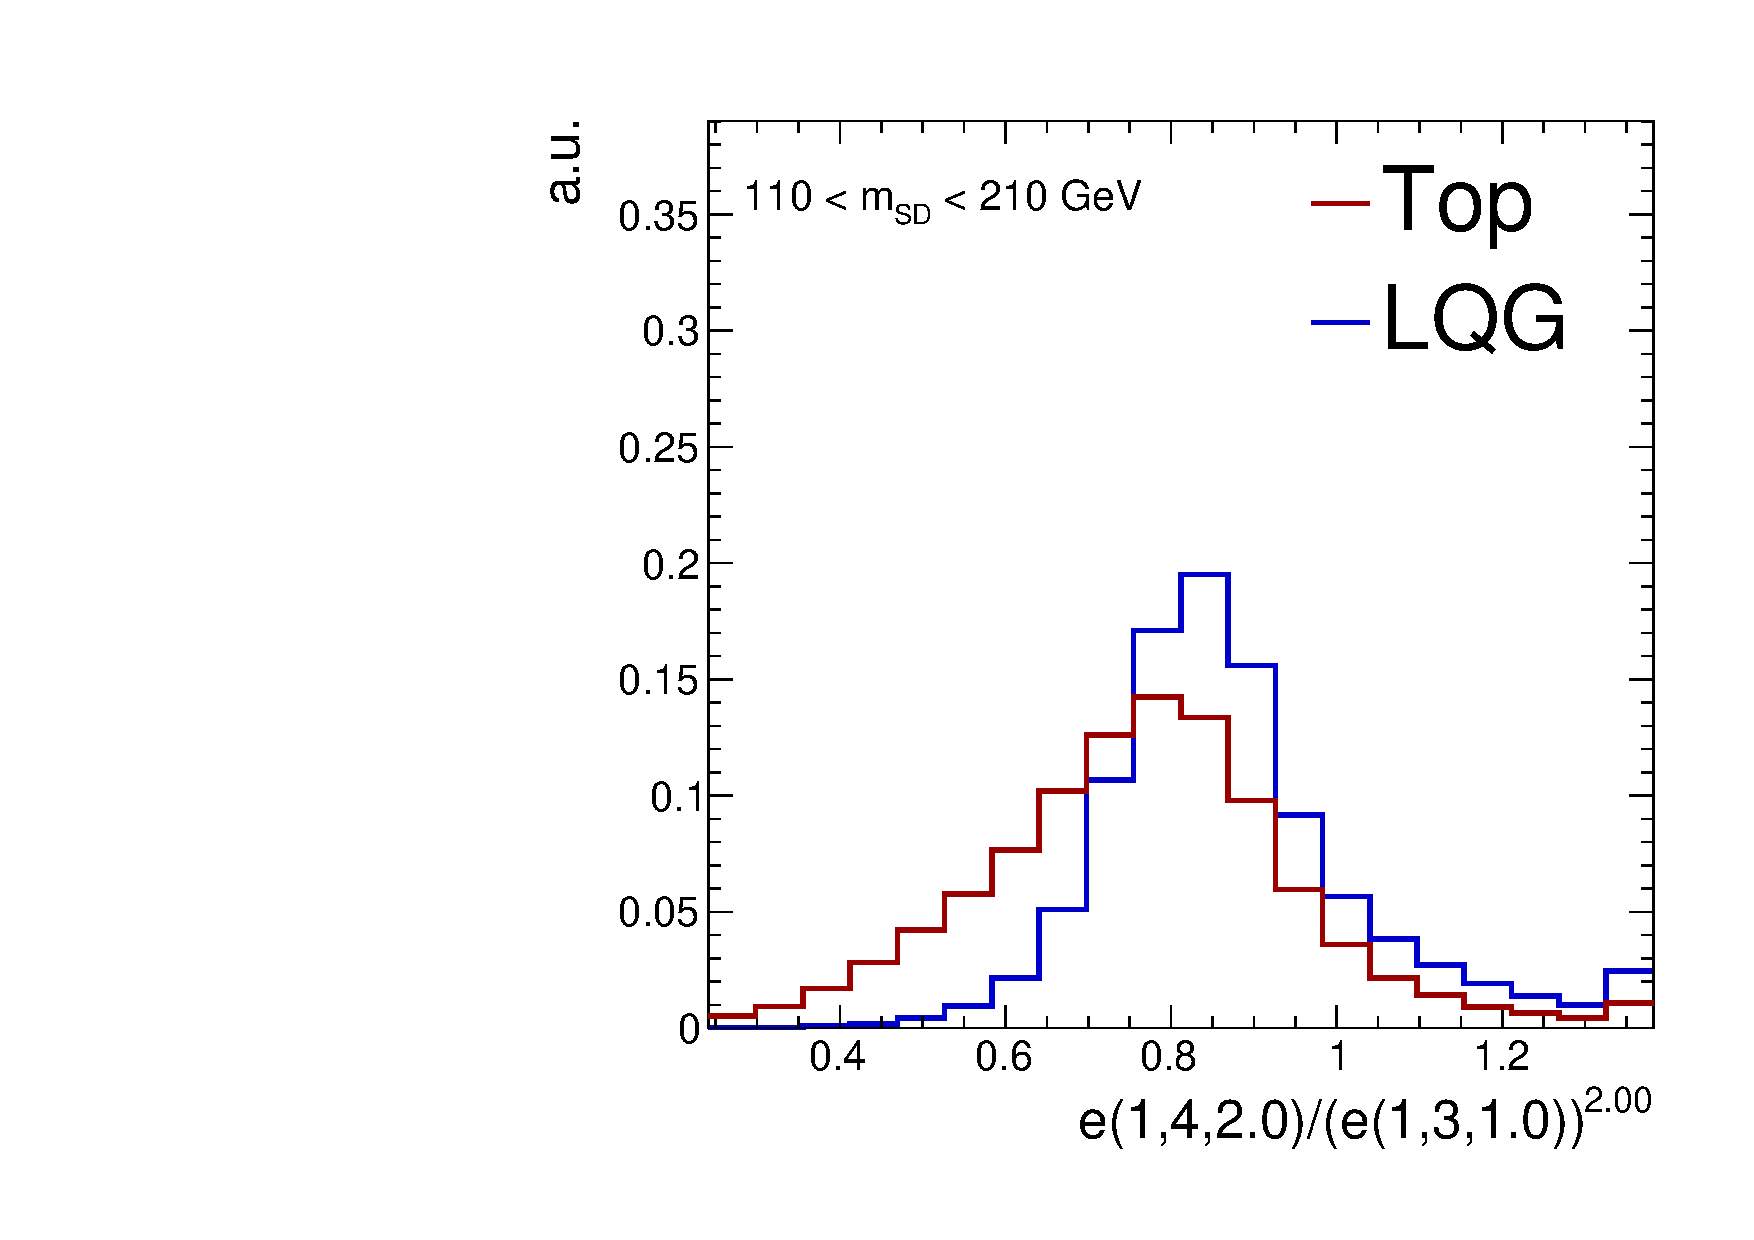
\includegraphics[width=0.24\textwidth]{figures/toptagging/shapes/mass_ratio_14201310.pdf}
        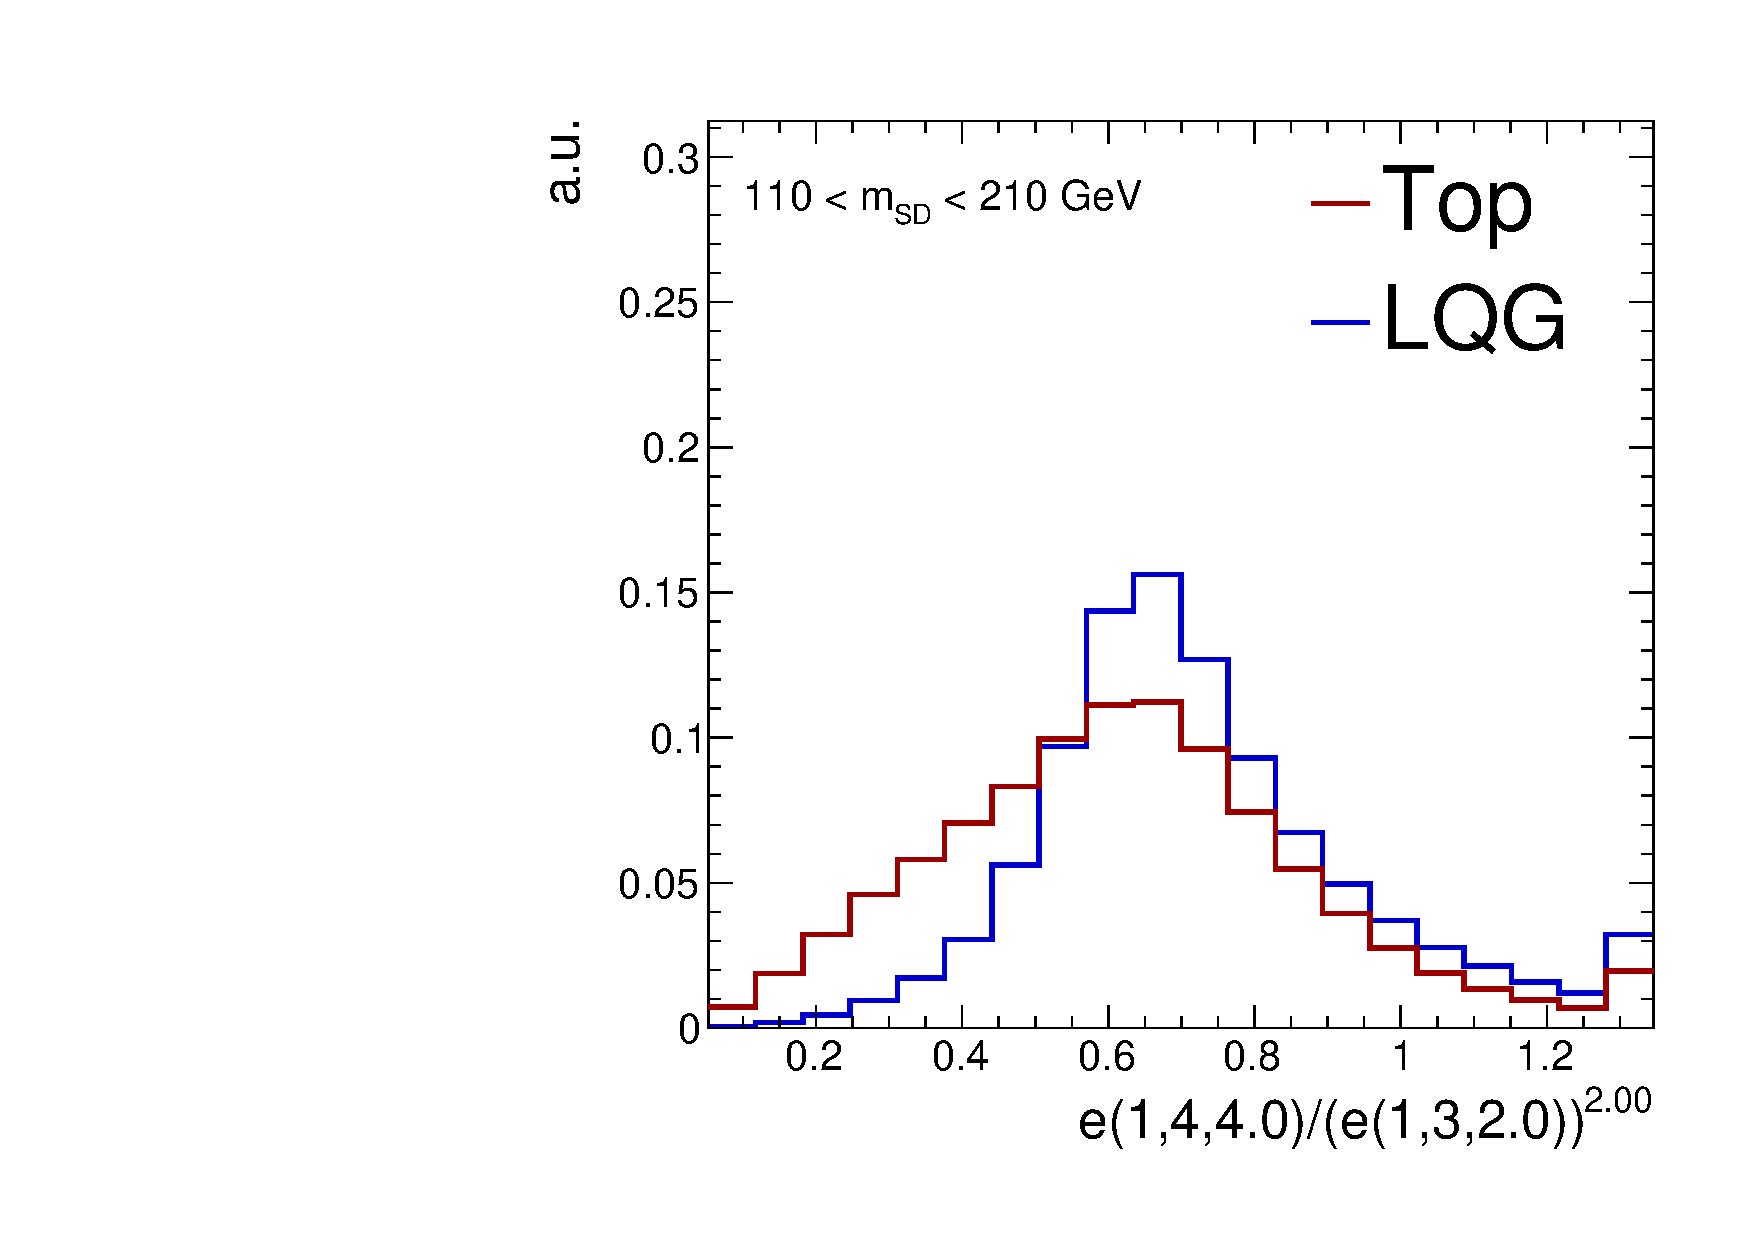
\includegraphics[width=0.24\textwidth]{figures/toptagging/shapes/mass_ratio_14401320.pdf}
        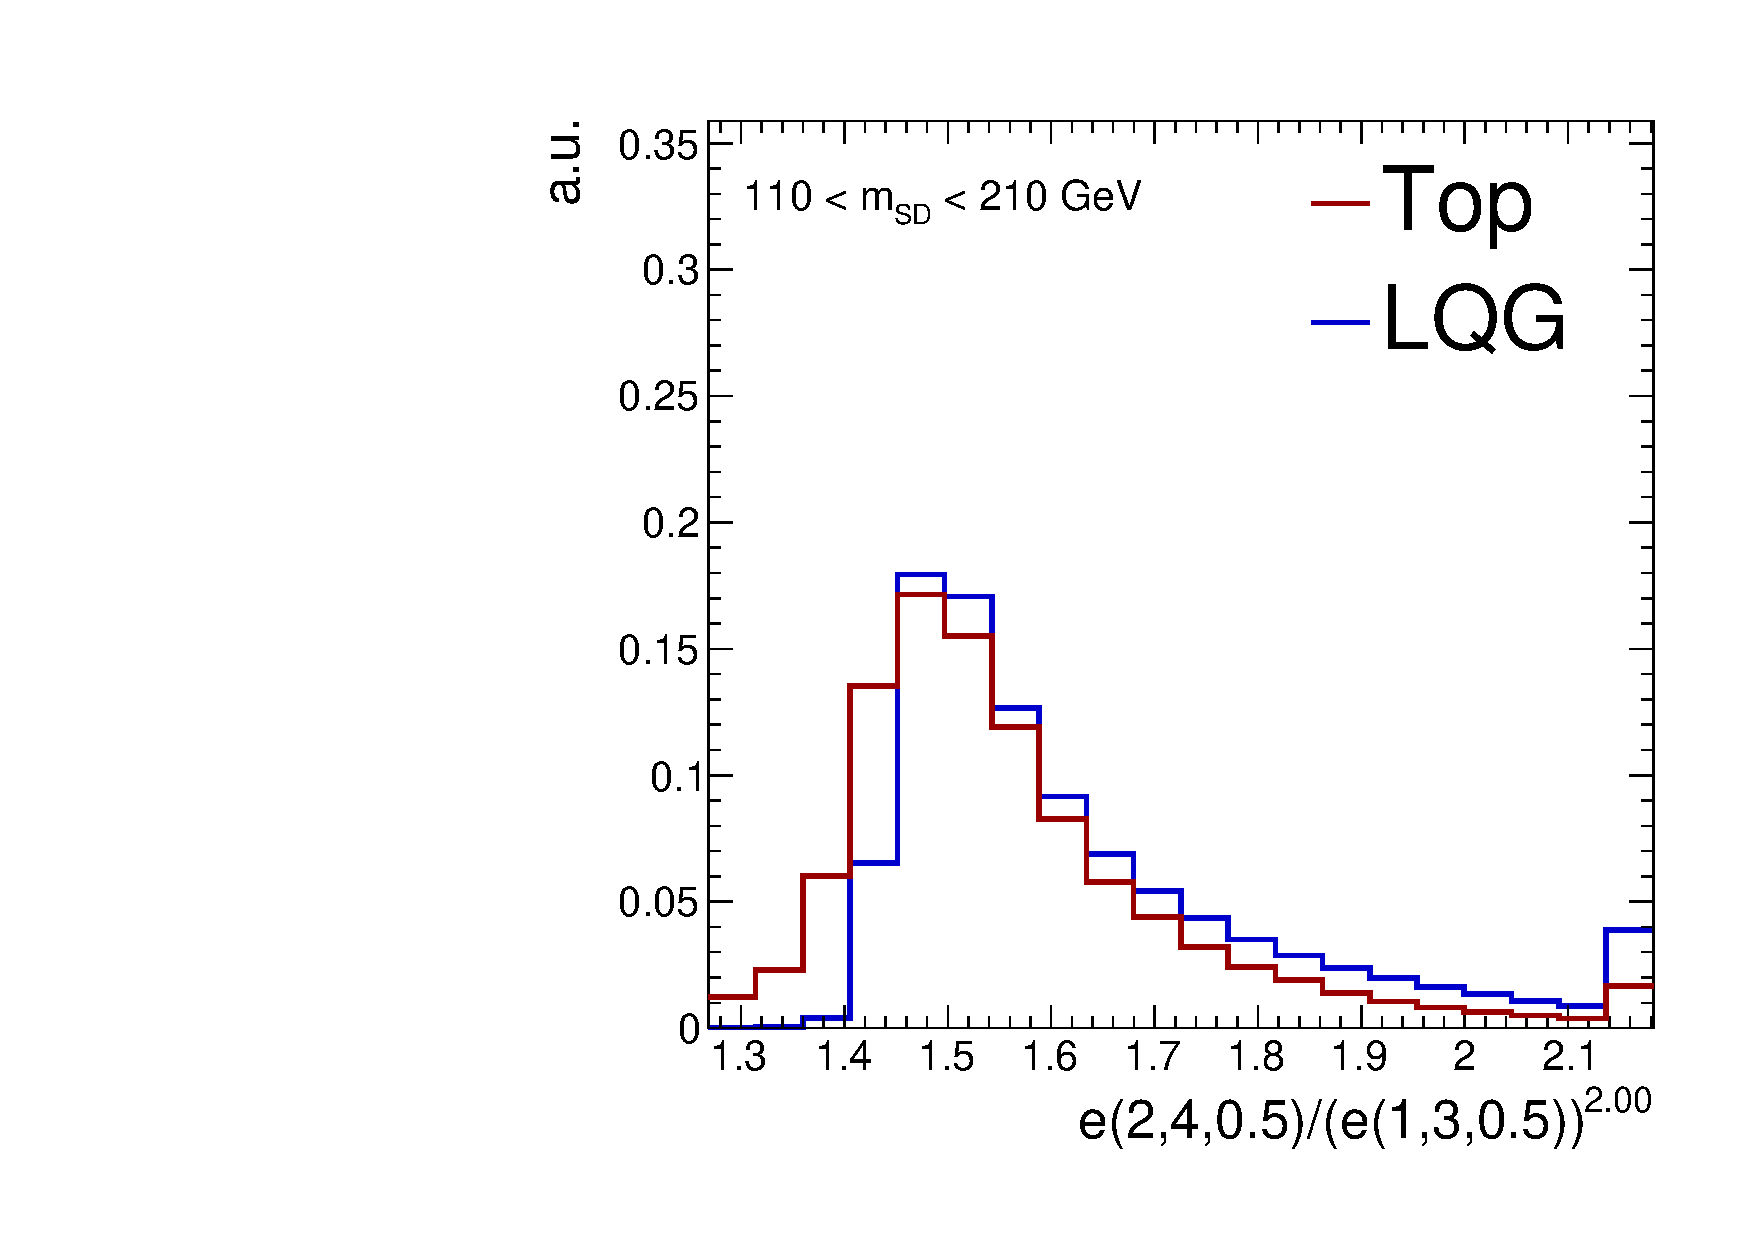
\includegraphics[width=0.24\textwidth]{figures/toptagging/shapes/mass_ratio_24051305.pdf}
        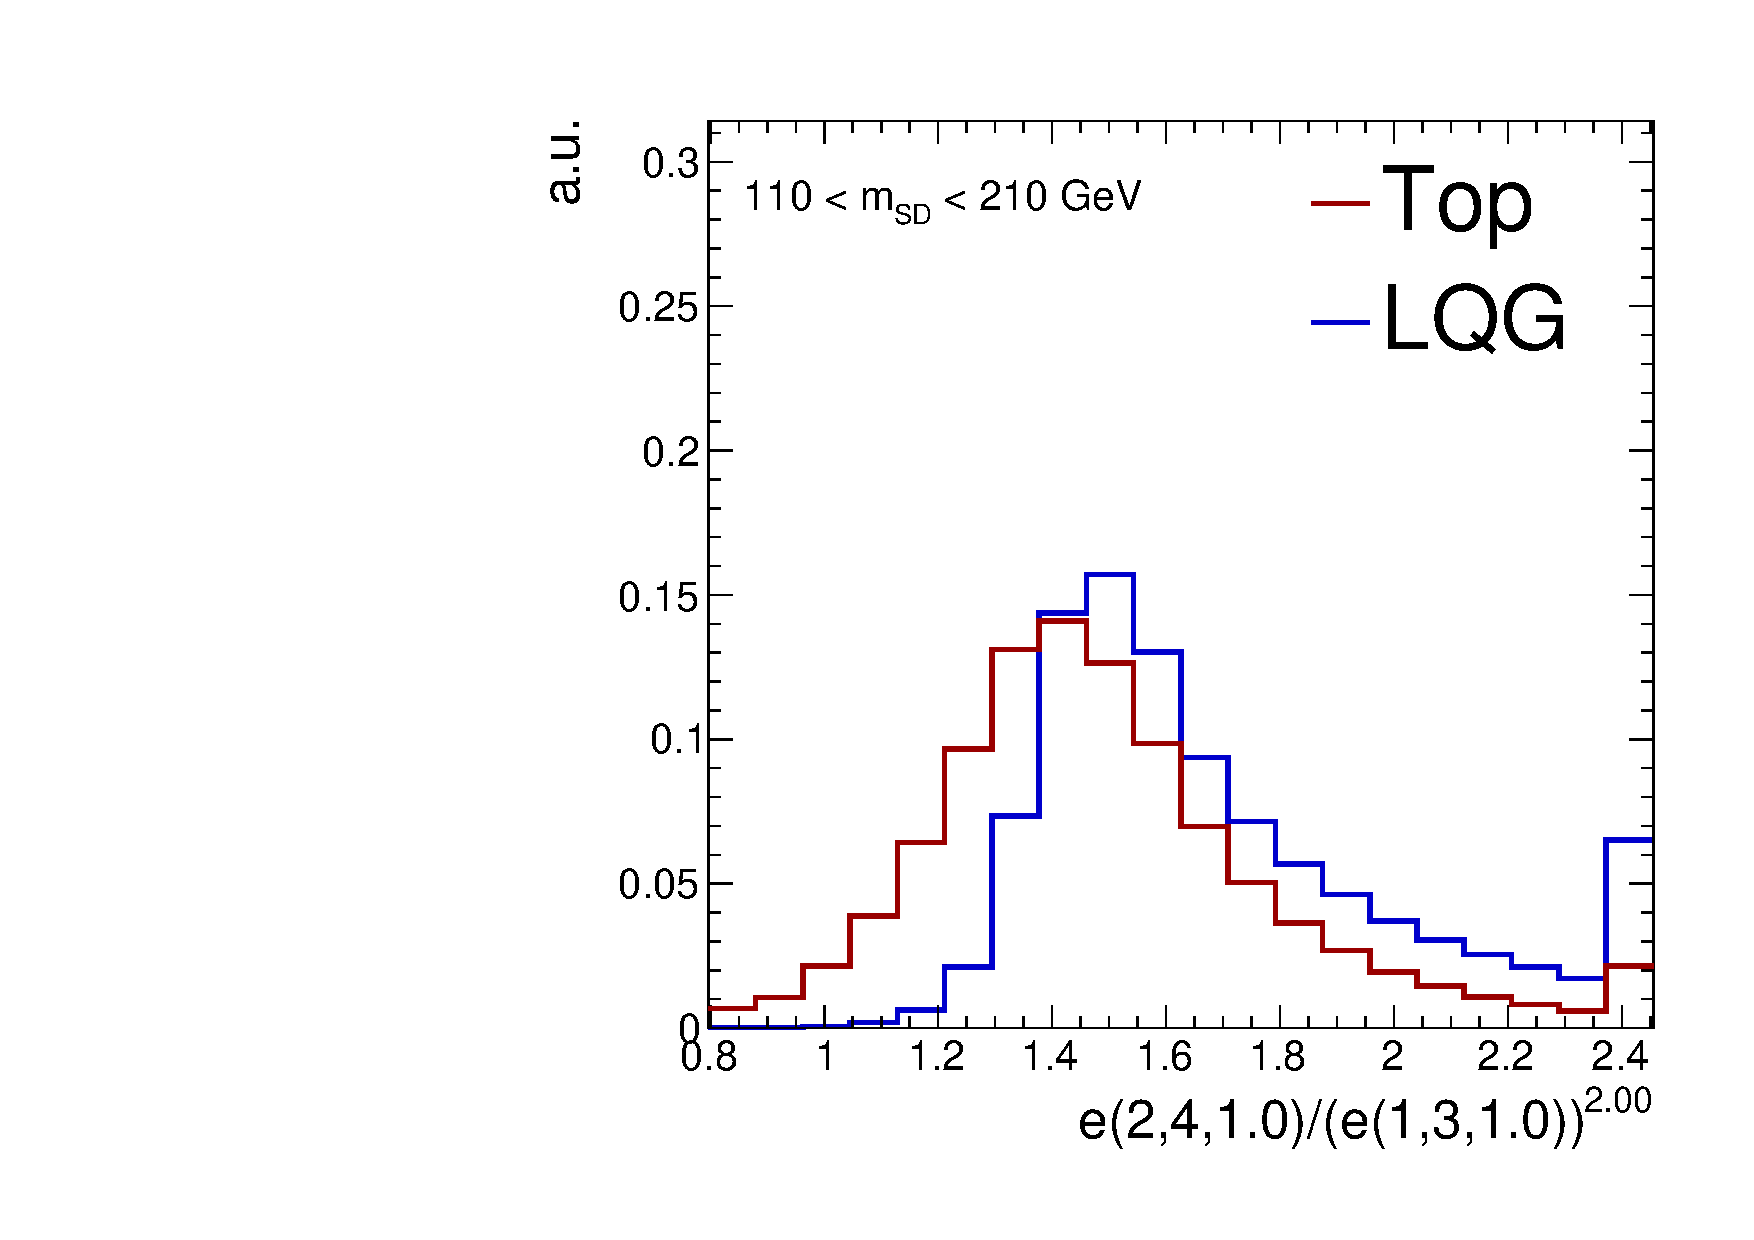
\includegraphics[width=0.24\textwidth]{figures/toptagging/shapes/mass_ratio_24101310.pdf}
        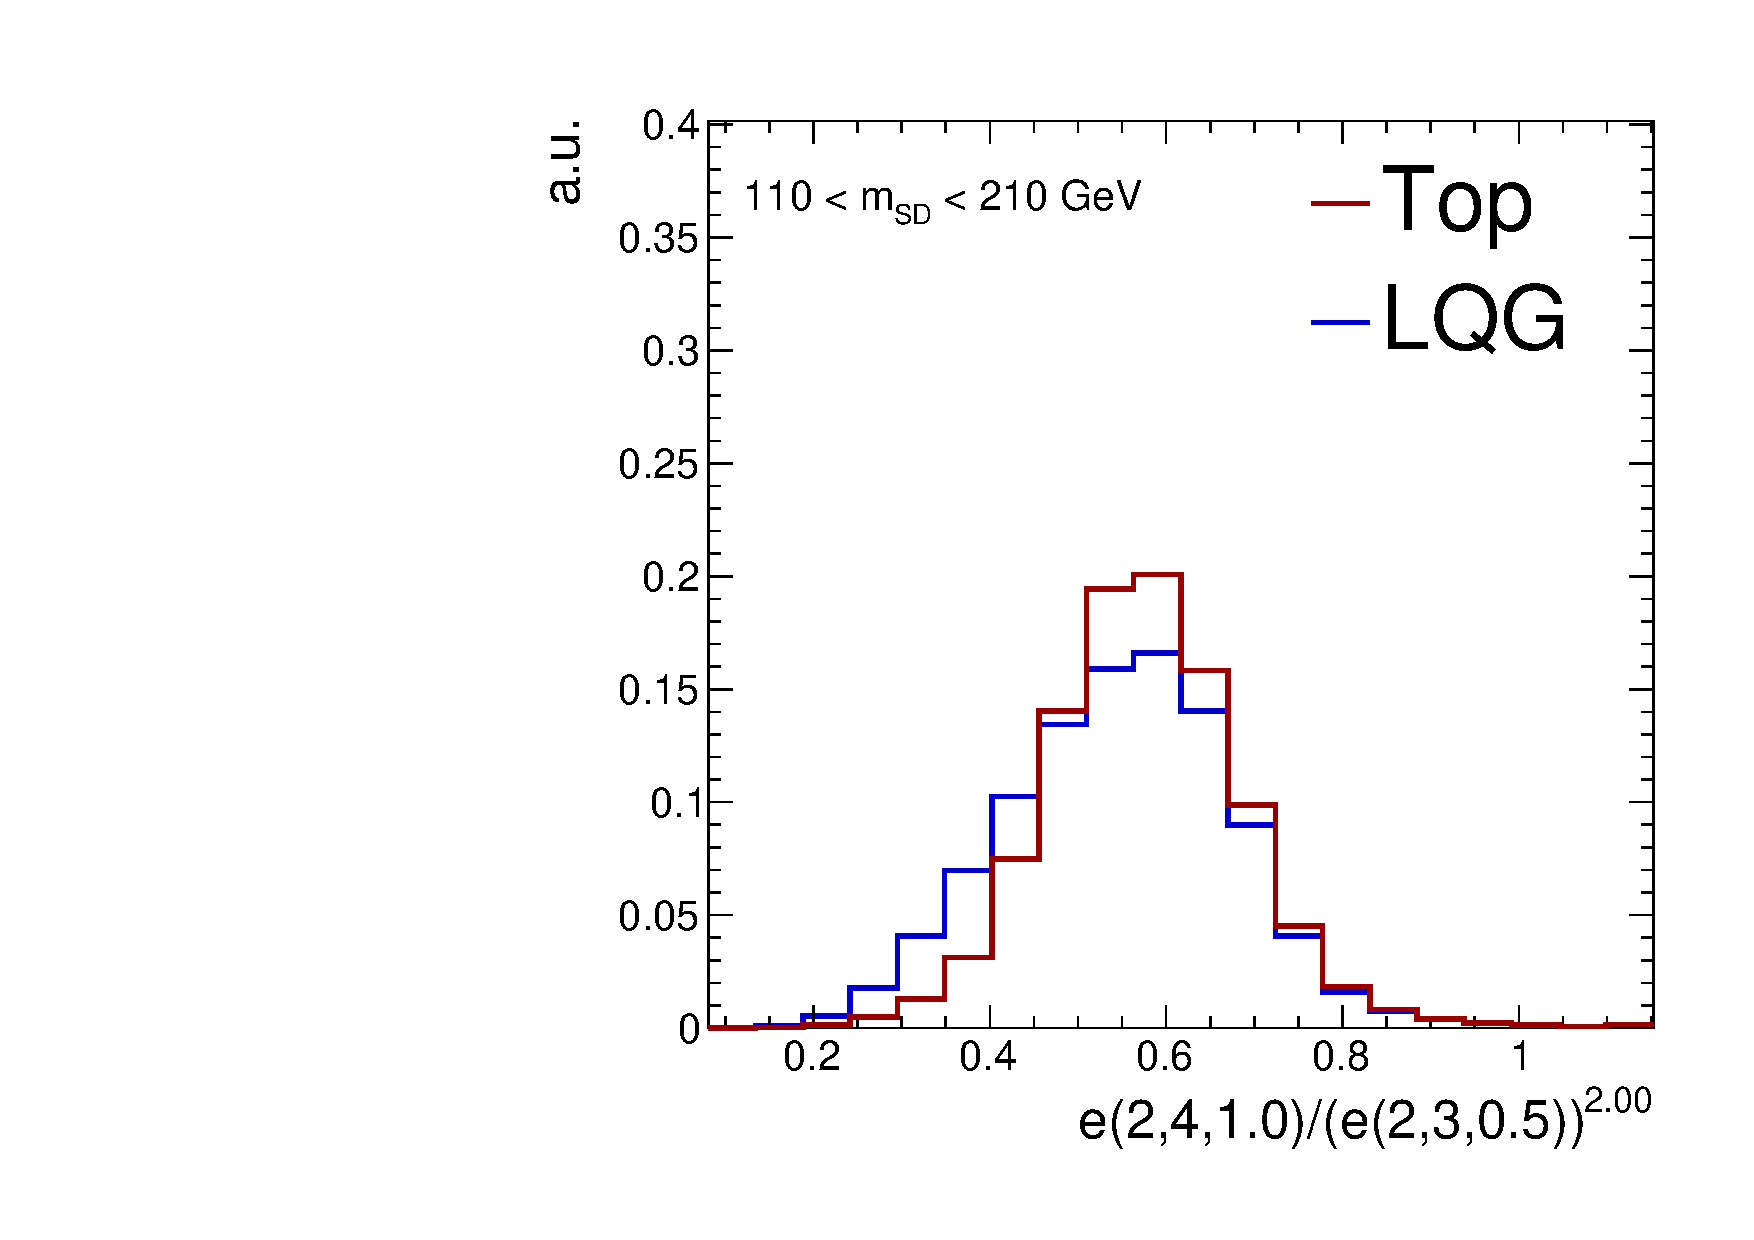
\includegraphics[width=0.24\textwidth]{figures/toptagging/shapes/mass_ratio_24102305.pdf}
        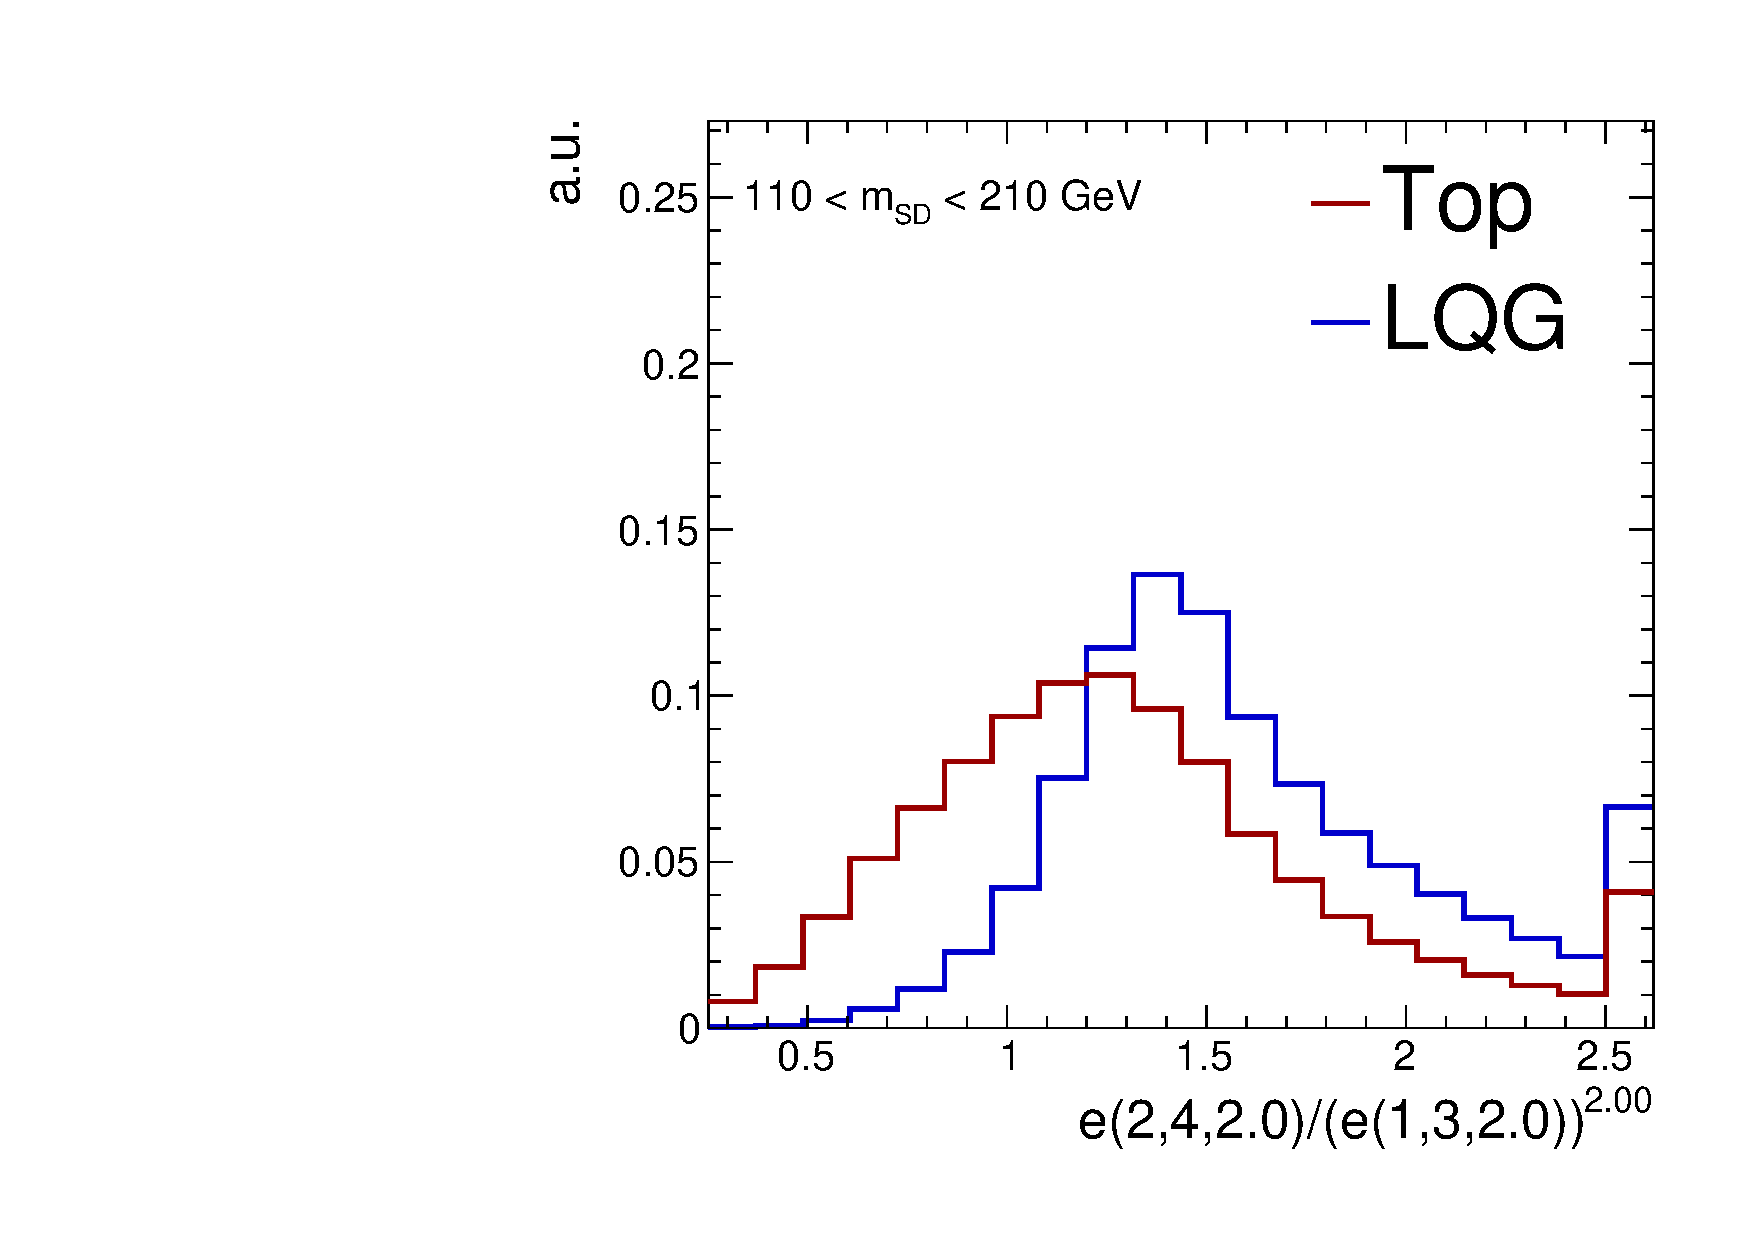
\includegraphics[width=0.24\textwidth]{figures/toptagging/shapes/mass_ratio_24201320.pdf}
        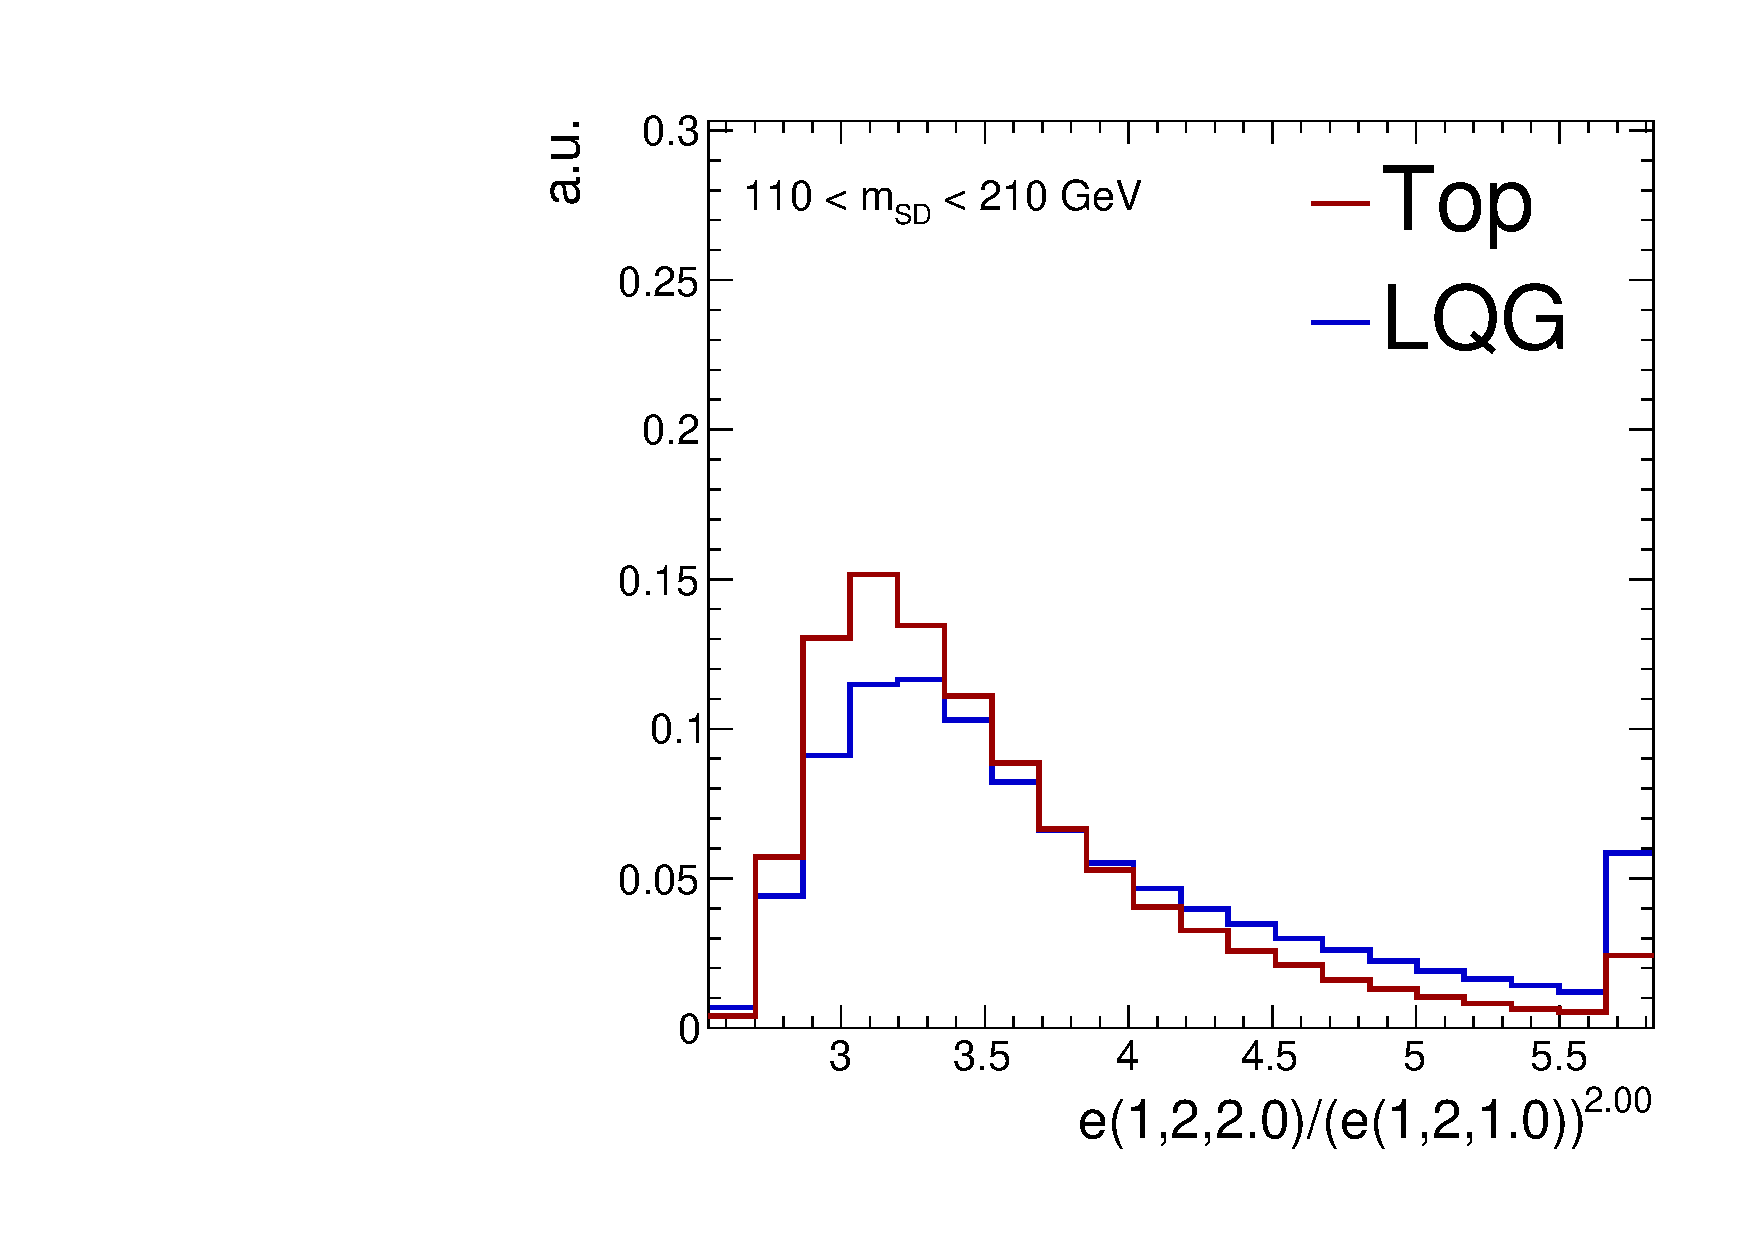
\includegraphics[width=0.24\textwidth]{figures/toptagging/shapes/mass_ratio_12201210.pdf}
        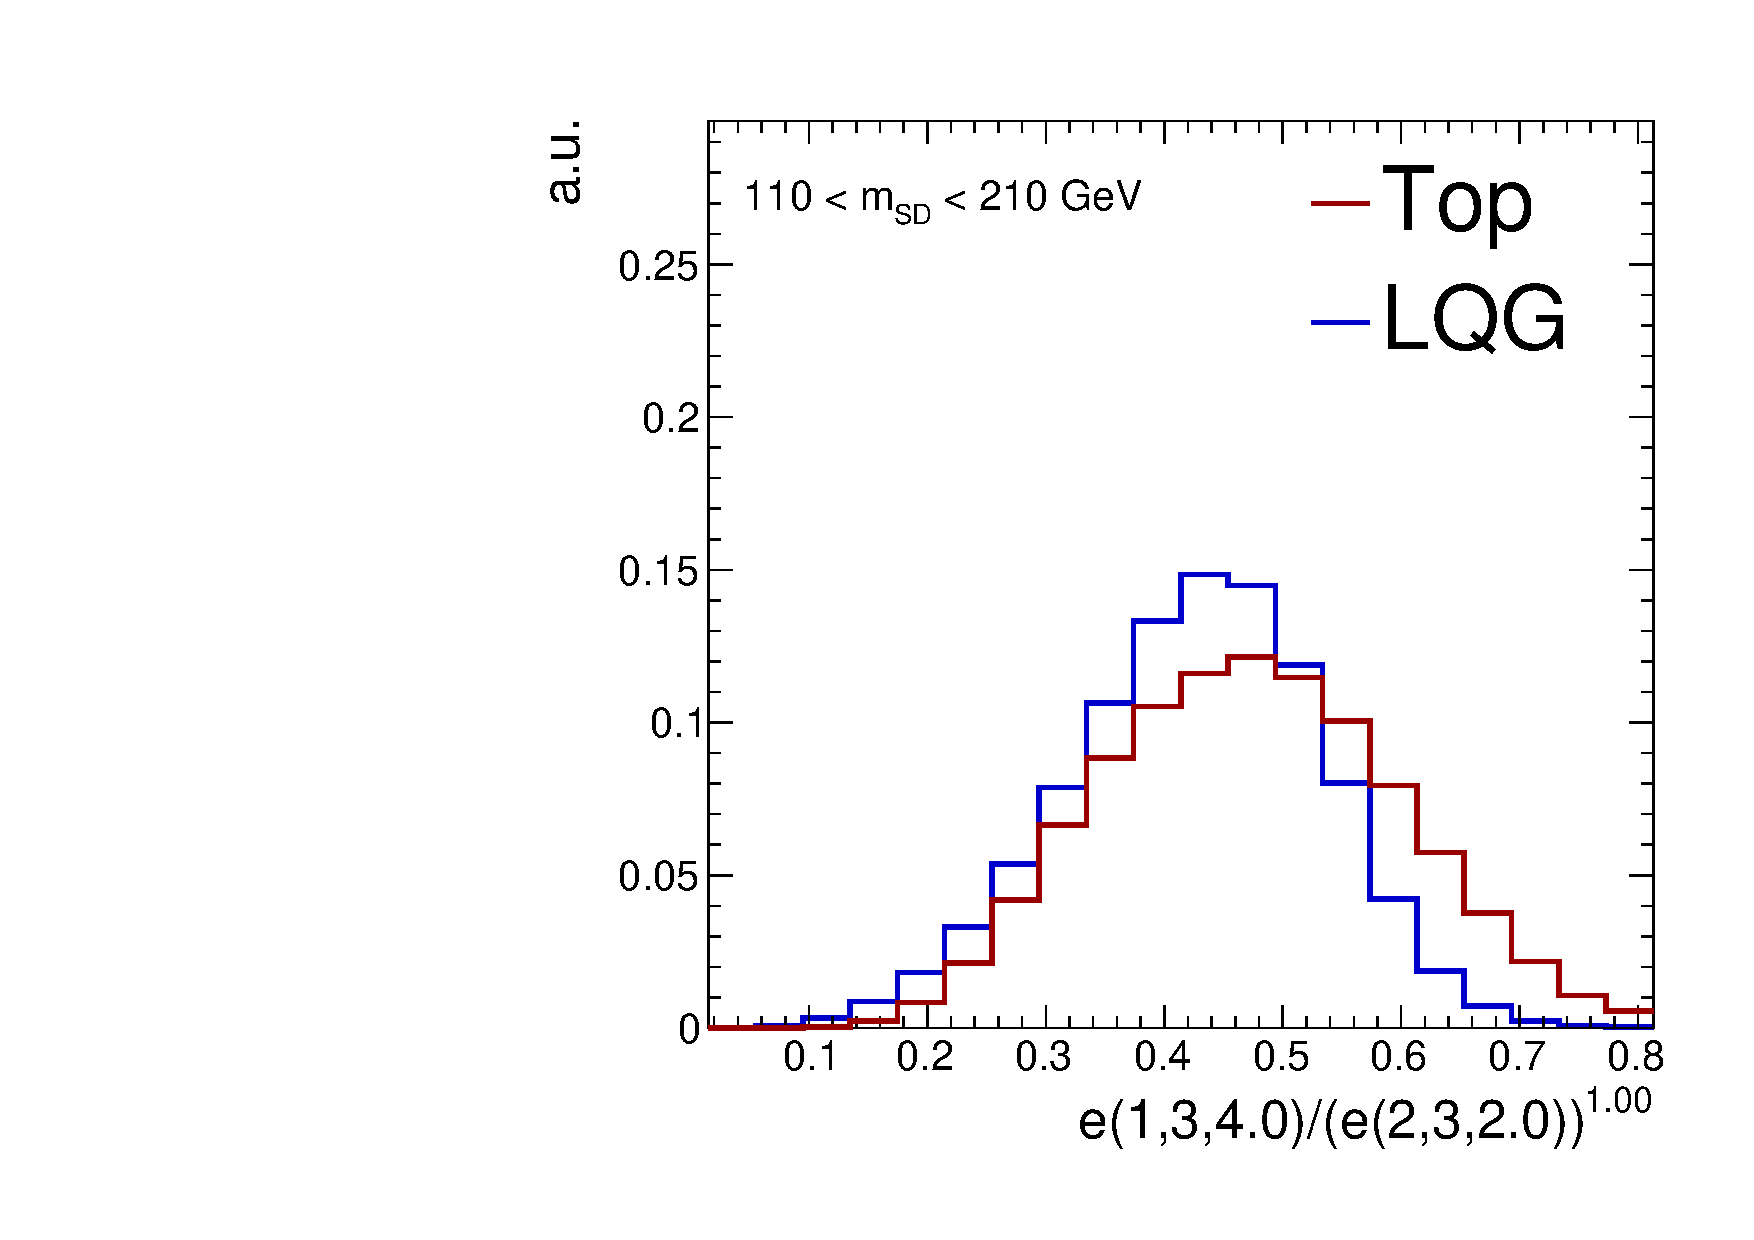
\includegraphics[width=0.24\textwidth]{figures/toptagging/shapes/mass_ratio_13402320.pdf}
        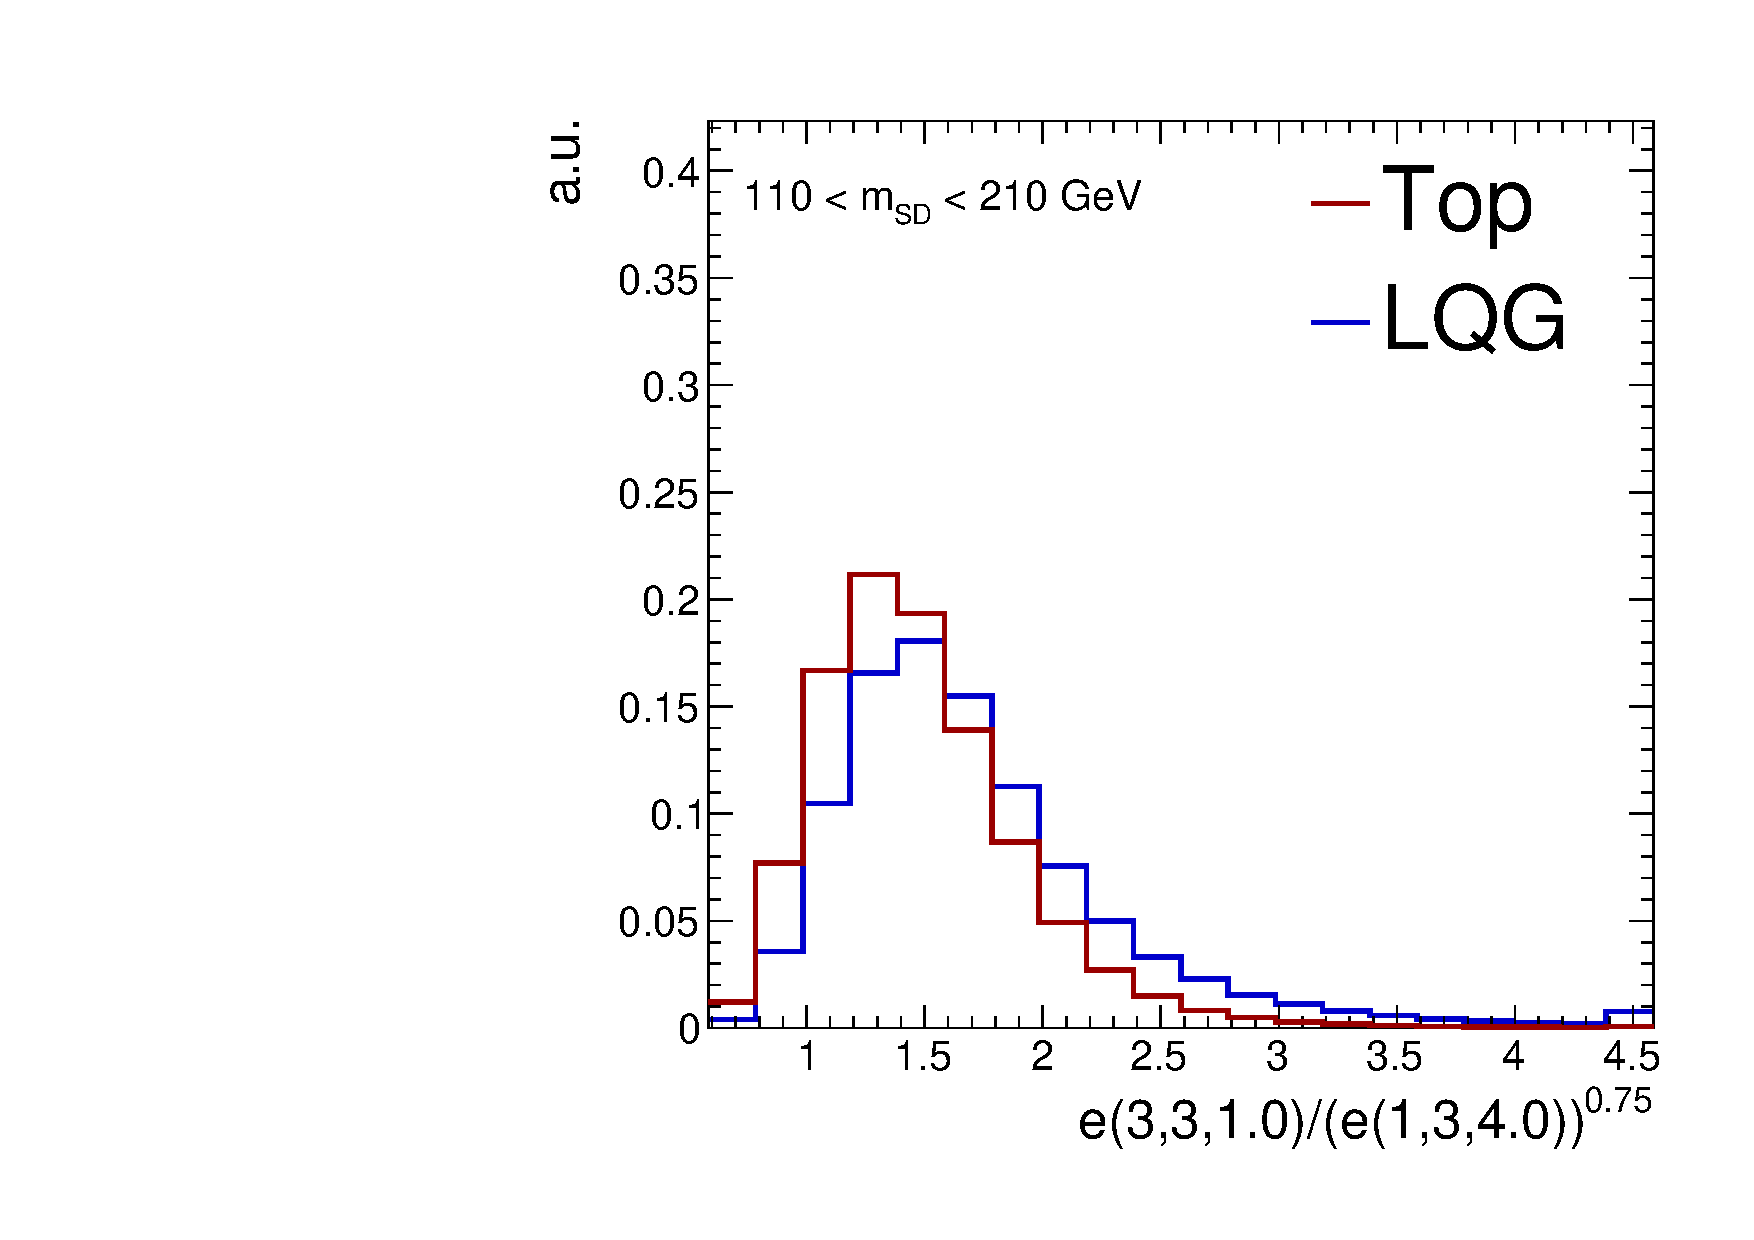
\includegraphics[width=0.24\textwidth]{figures/toptagging/shapes/mass_ratio_33101340.pdf}
        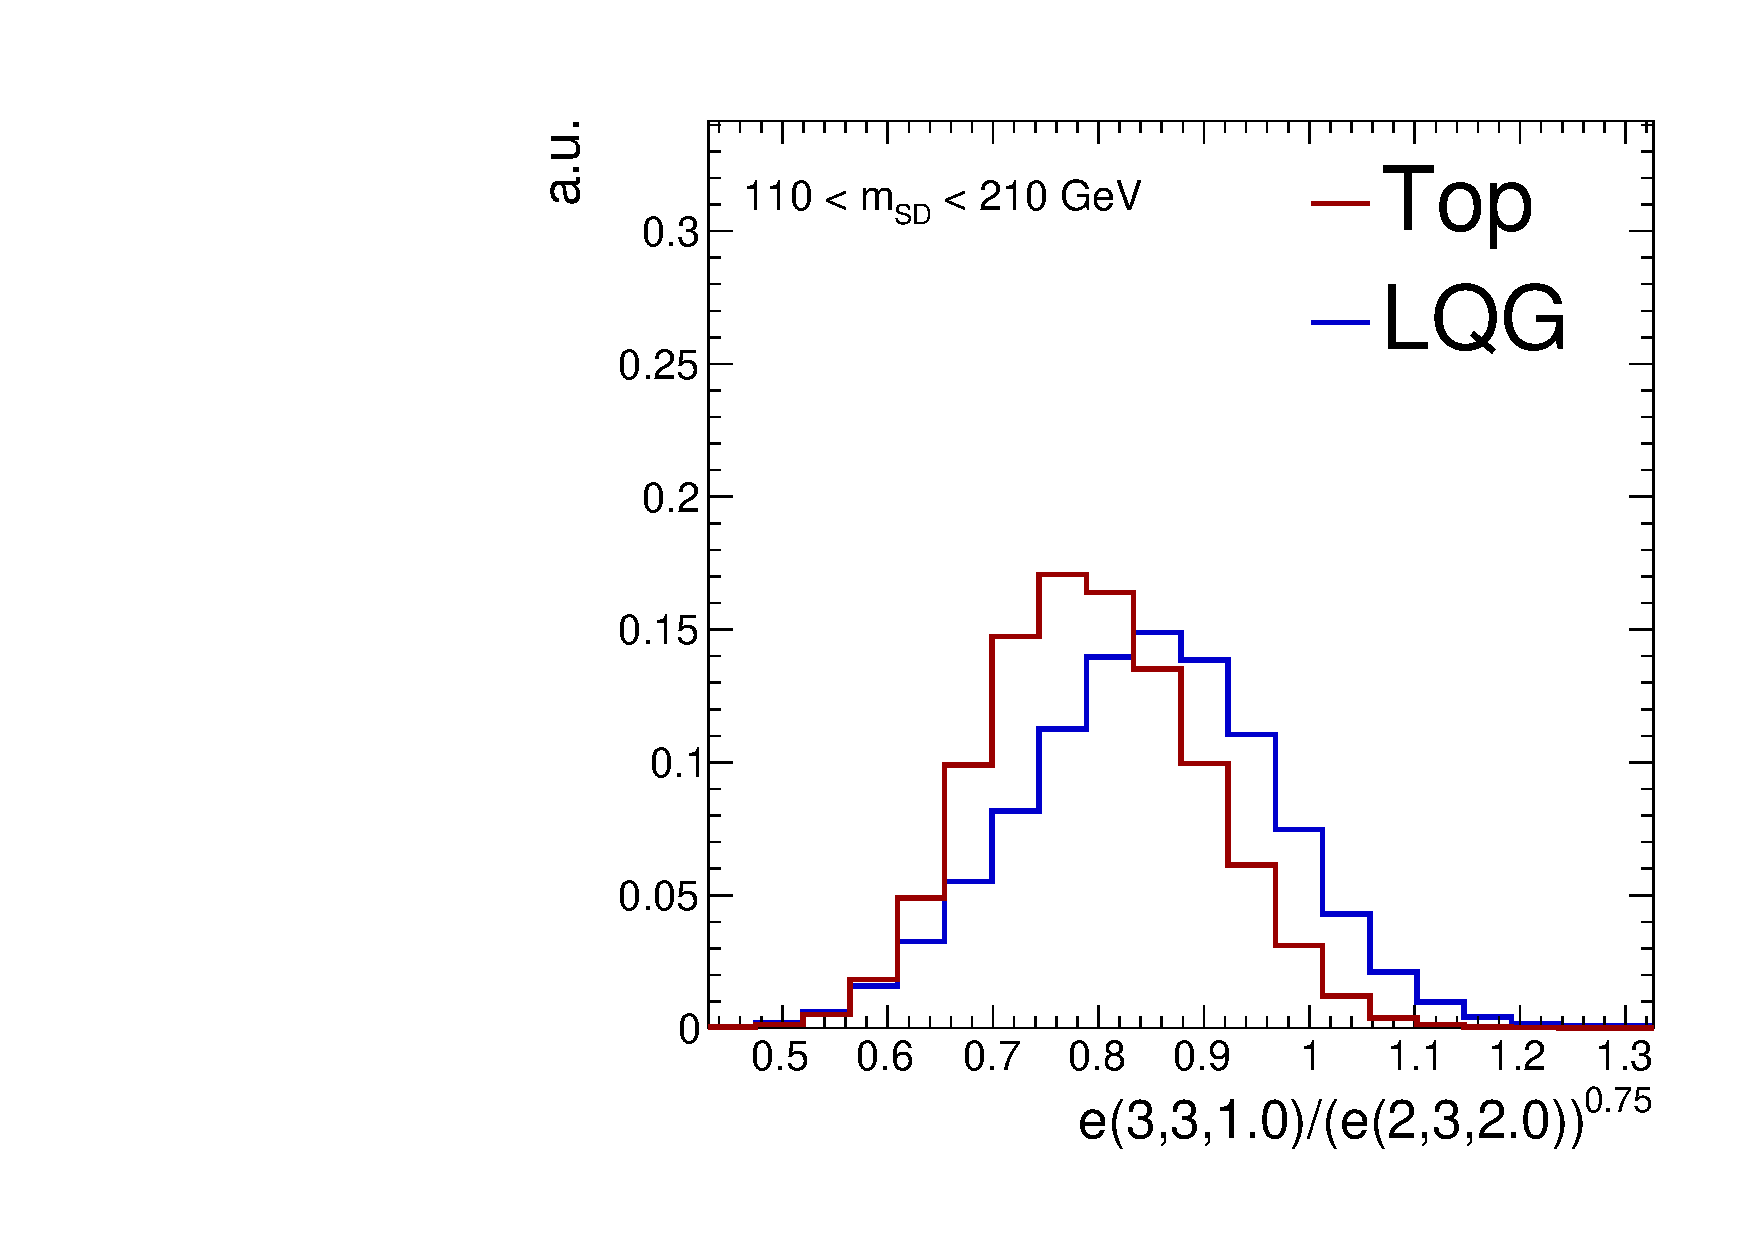
\includegraphics[width=0.24\textwidth]{figures/toptagging/shapes/mass_ratio_33102320.pdf}
        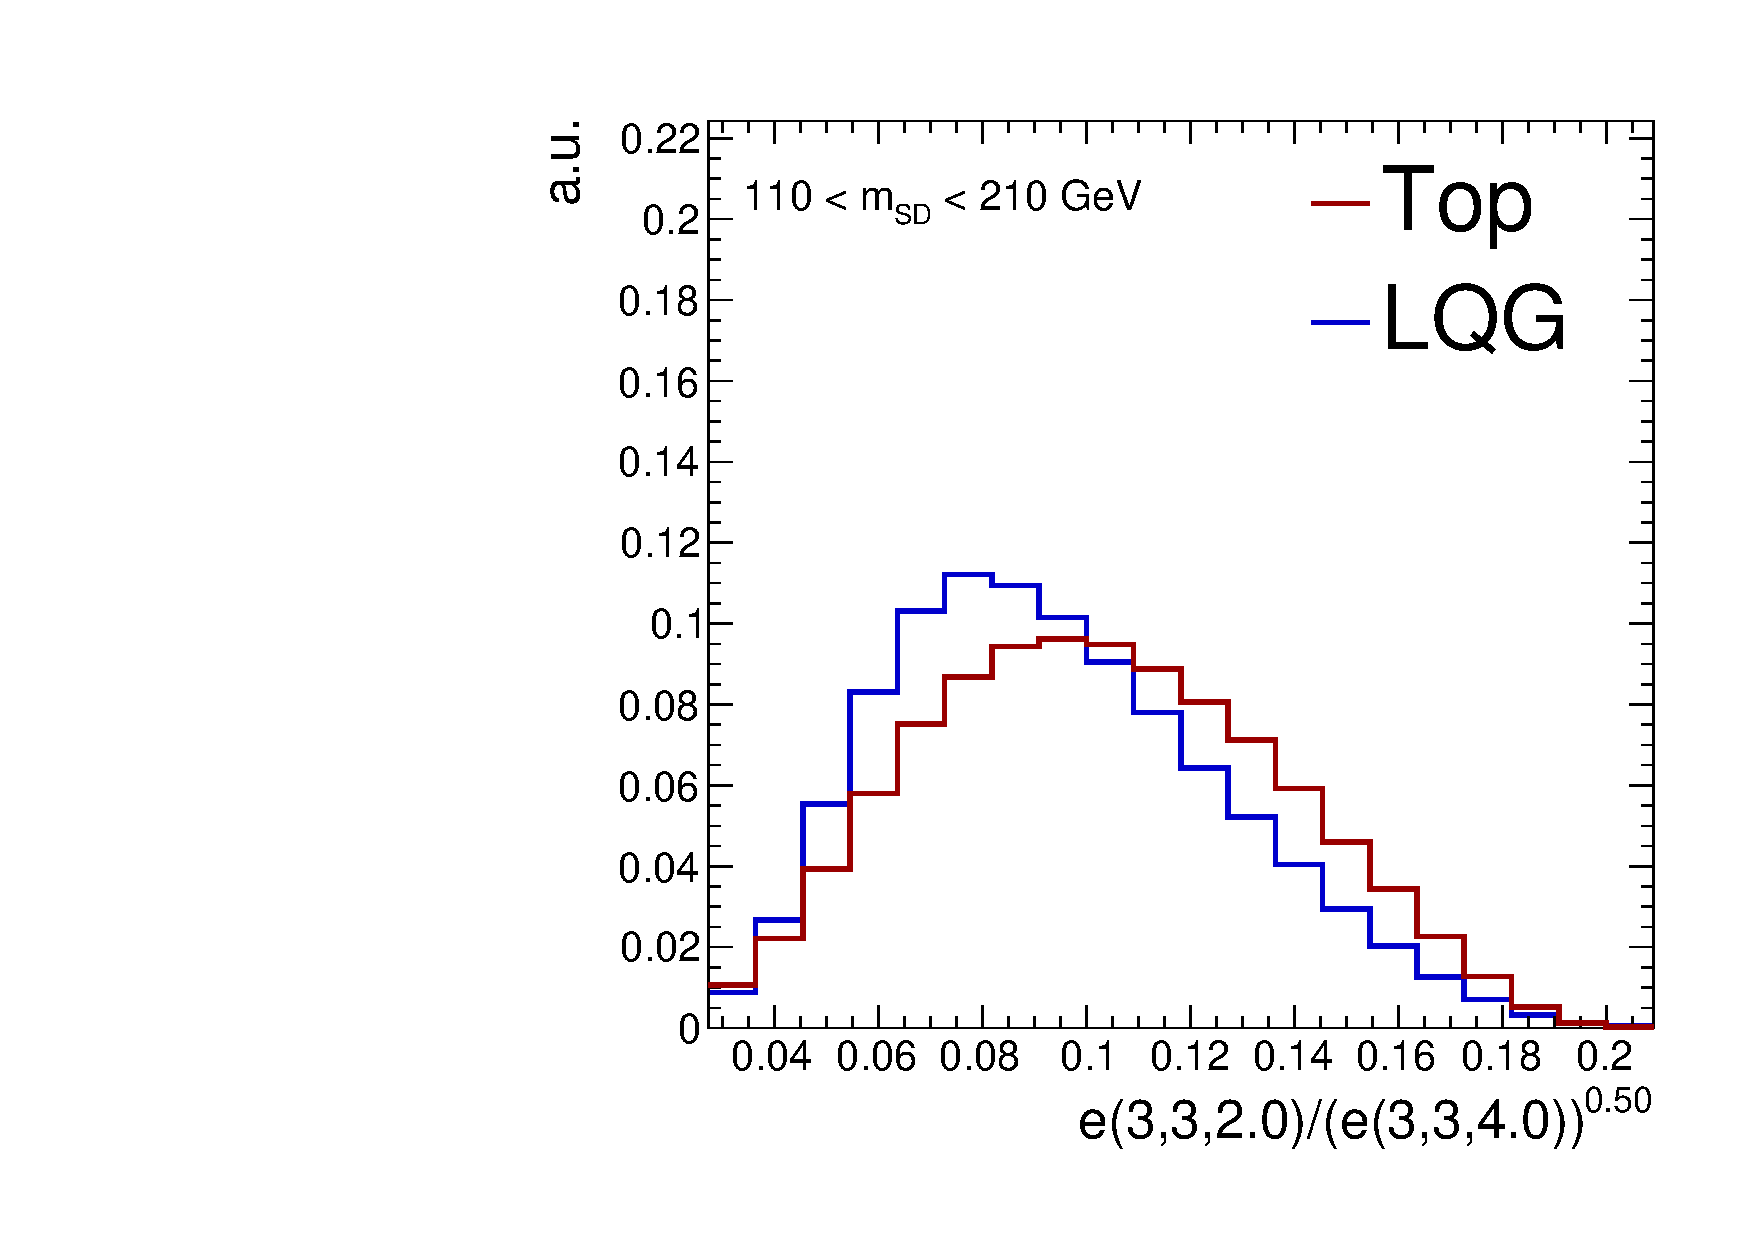
\includegraphics[width=0.24\textwidth]{figures/toptagging/shapes/mass_ratio_33203340.pdf} \\ 
        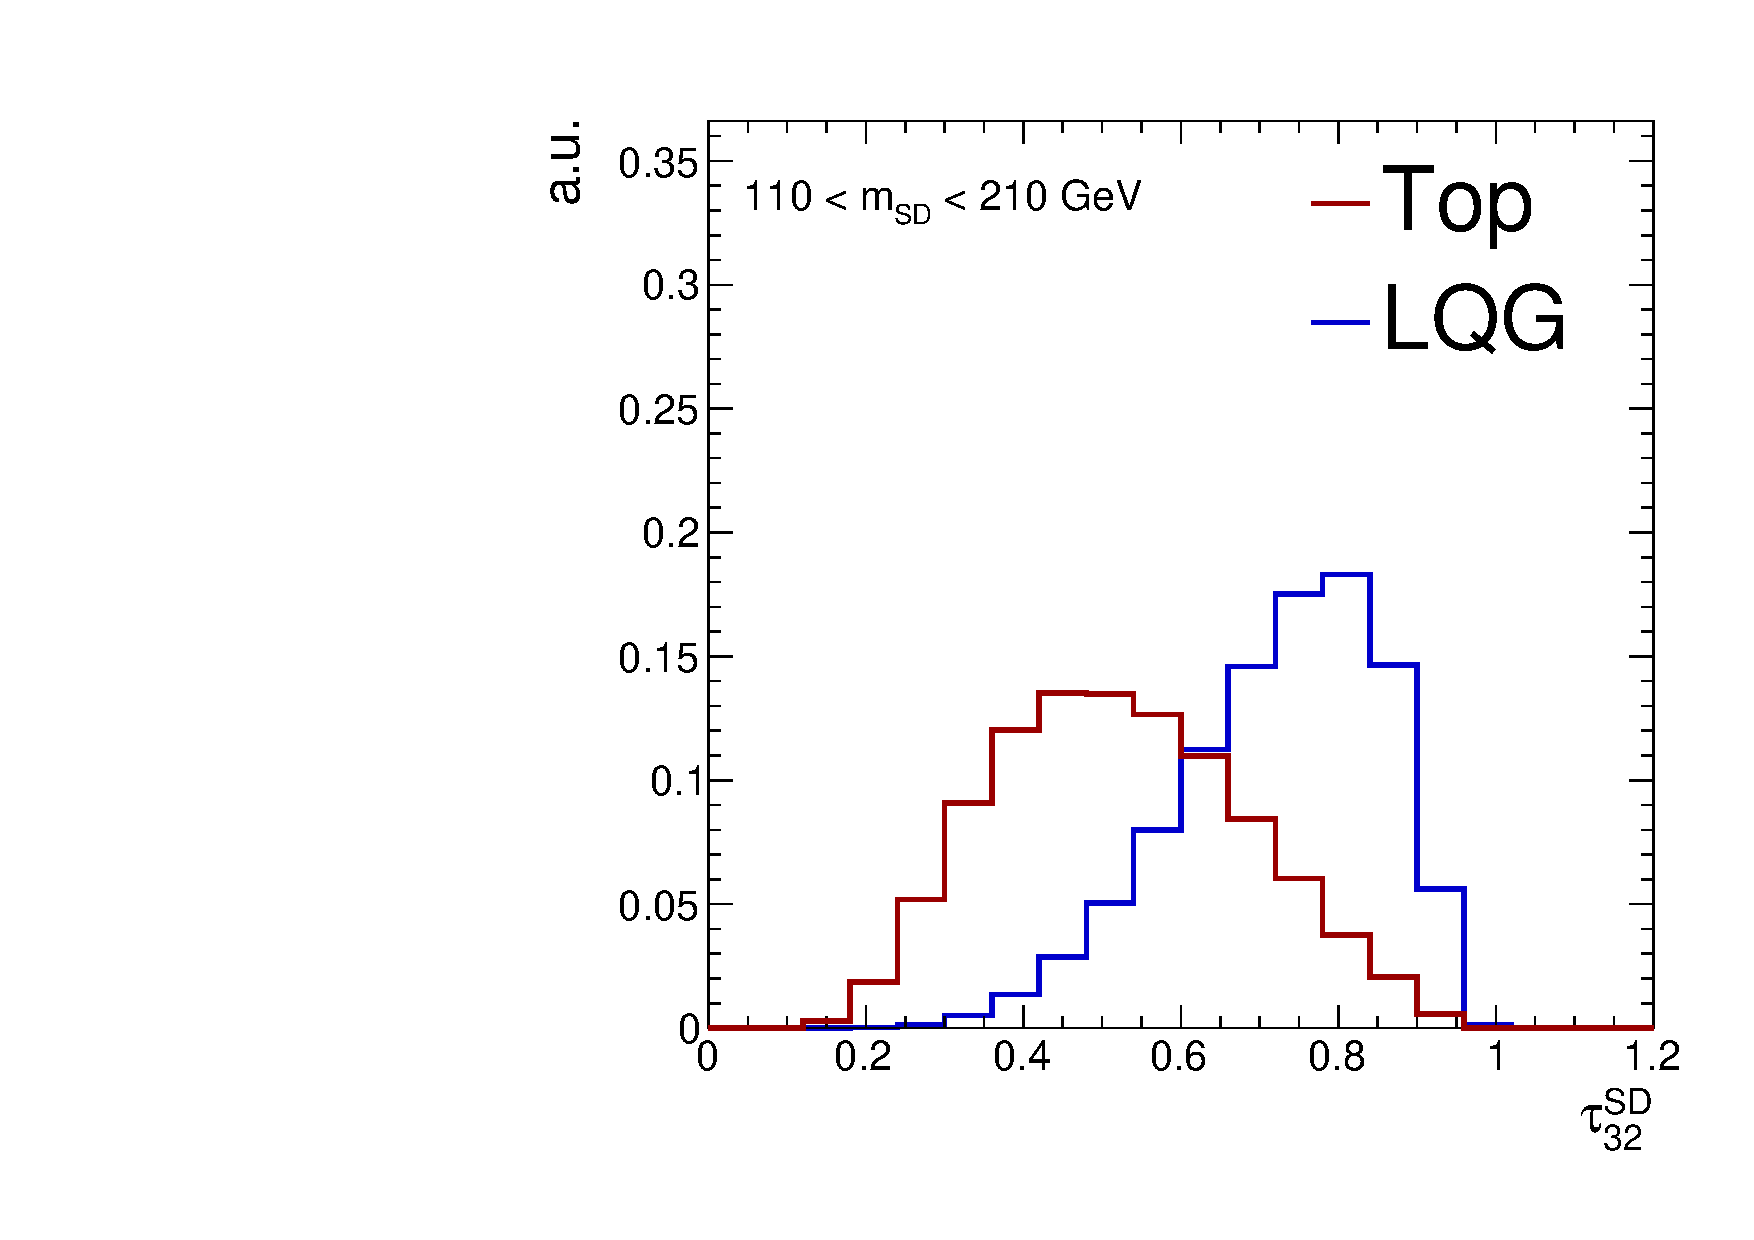
\includegraphics[width=0.24\textwidth]{figures/toptagging/shapes/mass_fjTau32SD.pdf}
        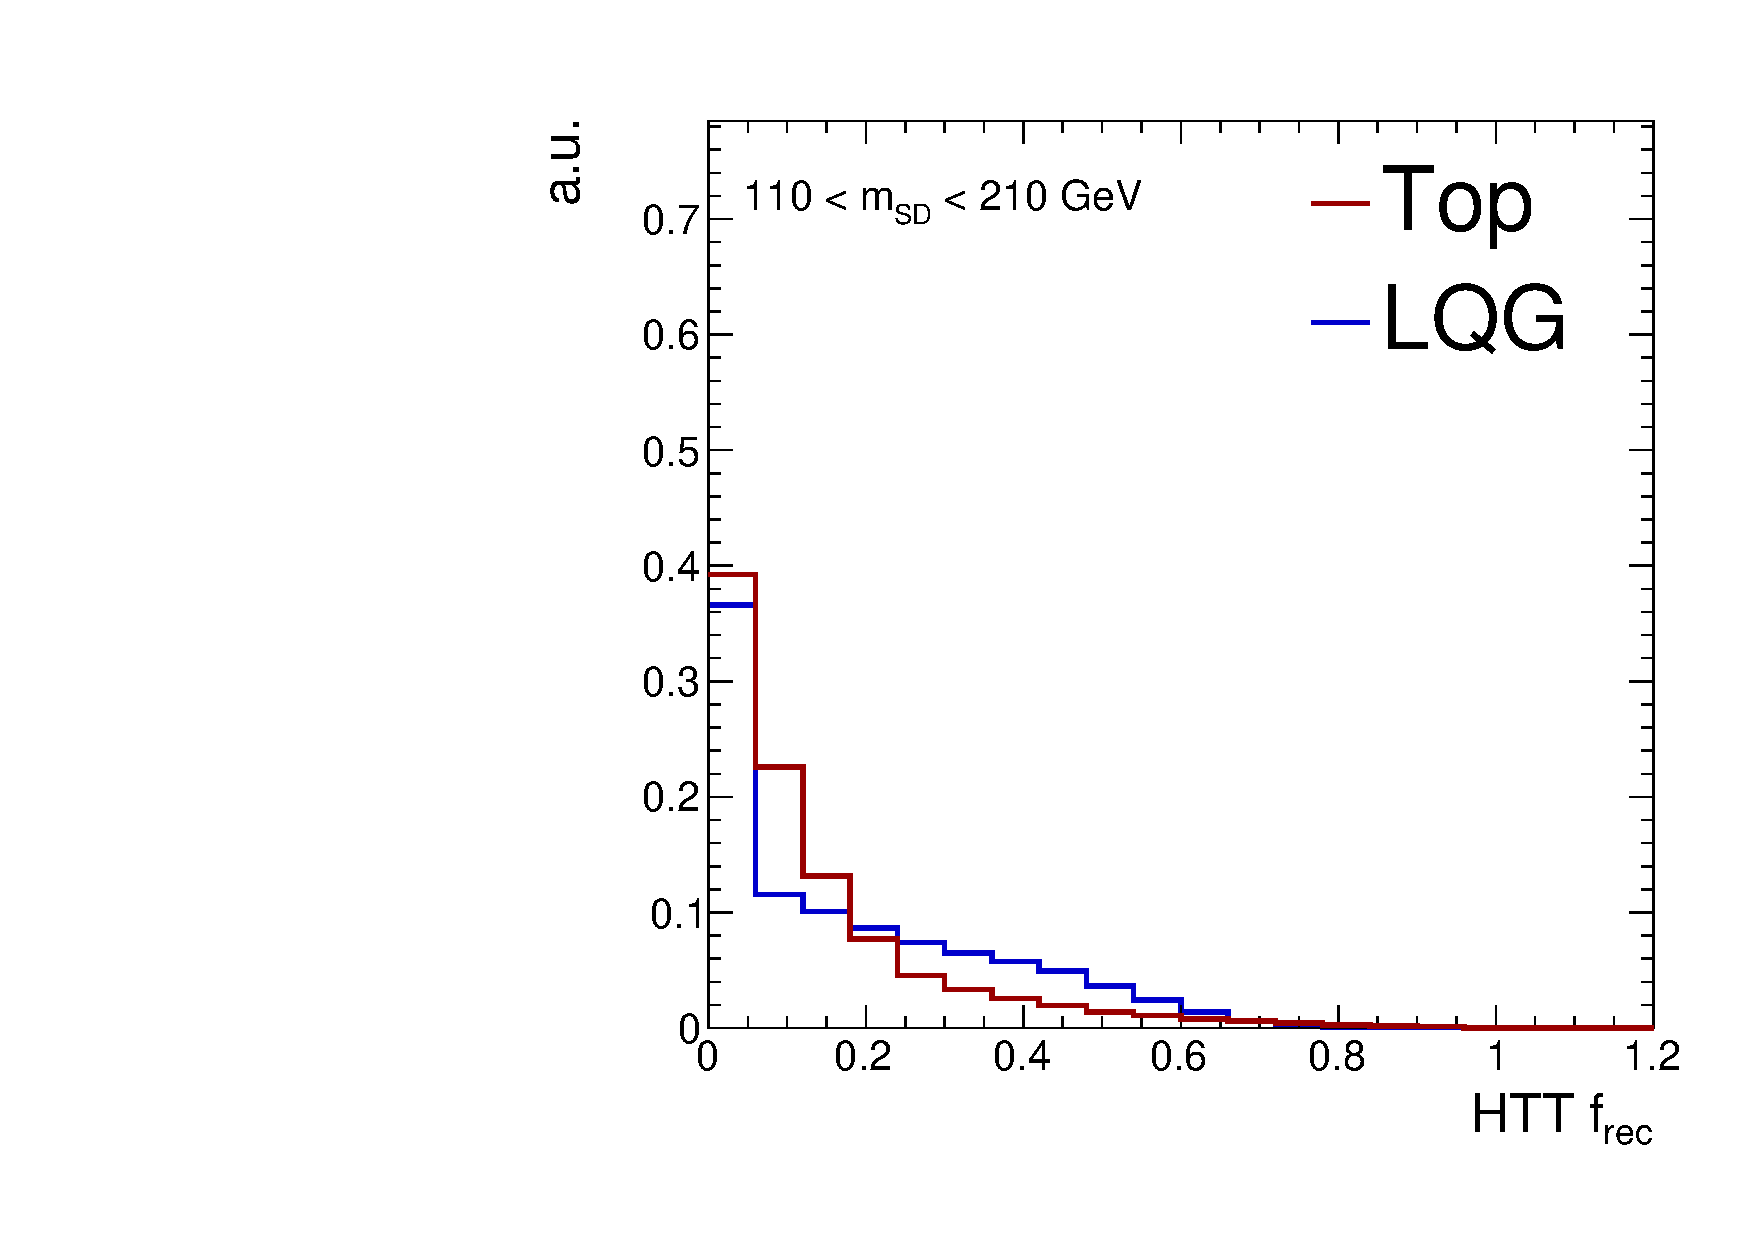
\includegraphics[width=0.24\textwidth]{figures/toptagging/shapes/mass_fjHTTFRec.pdf}
        \caption{Distributions of the 13 features selected by the iterative BDT training}
        \label{fig:jets:features}
    \end{center}
\end{figure}

\begin{figure}[]
    \begin{center}
        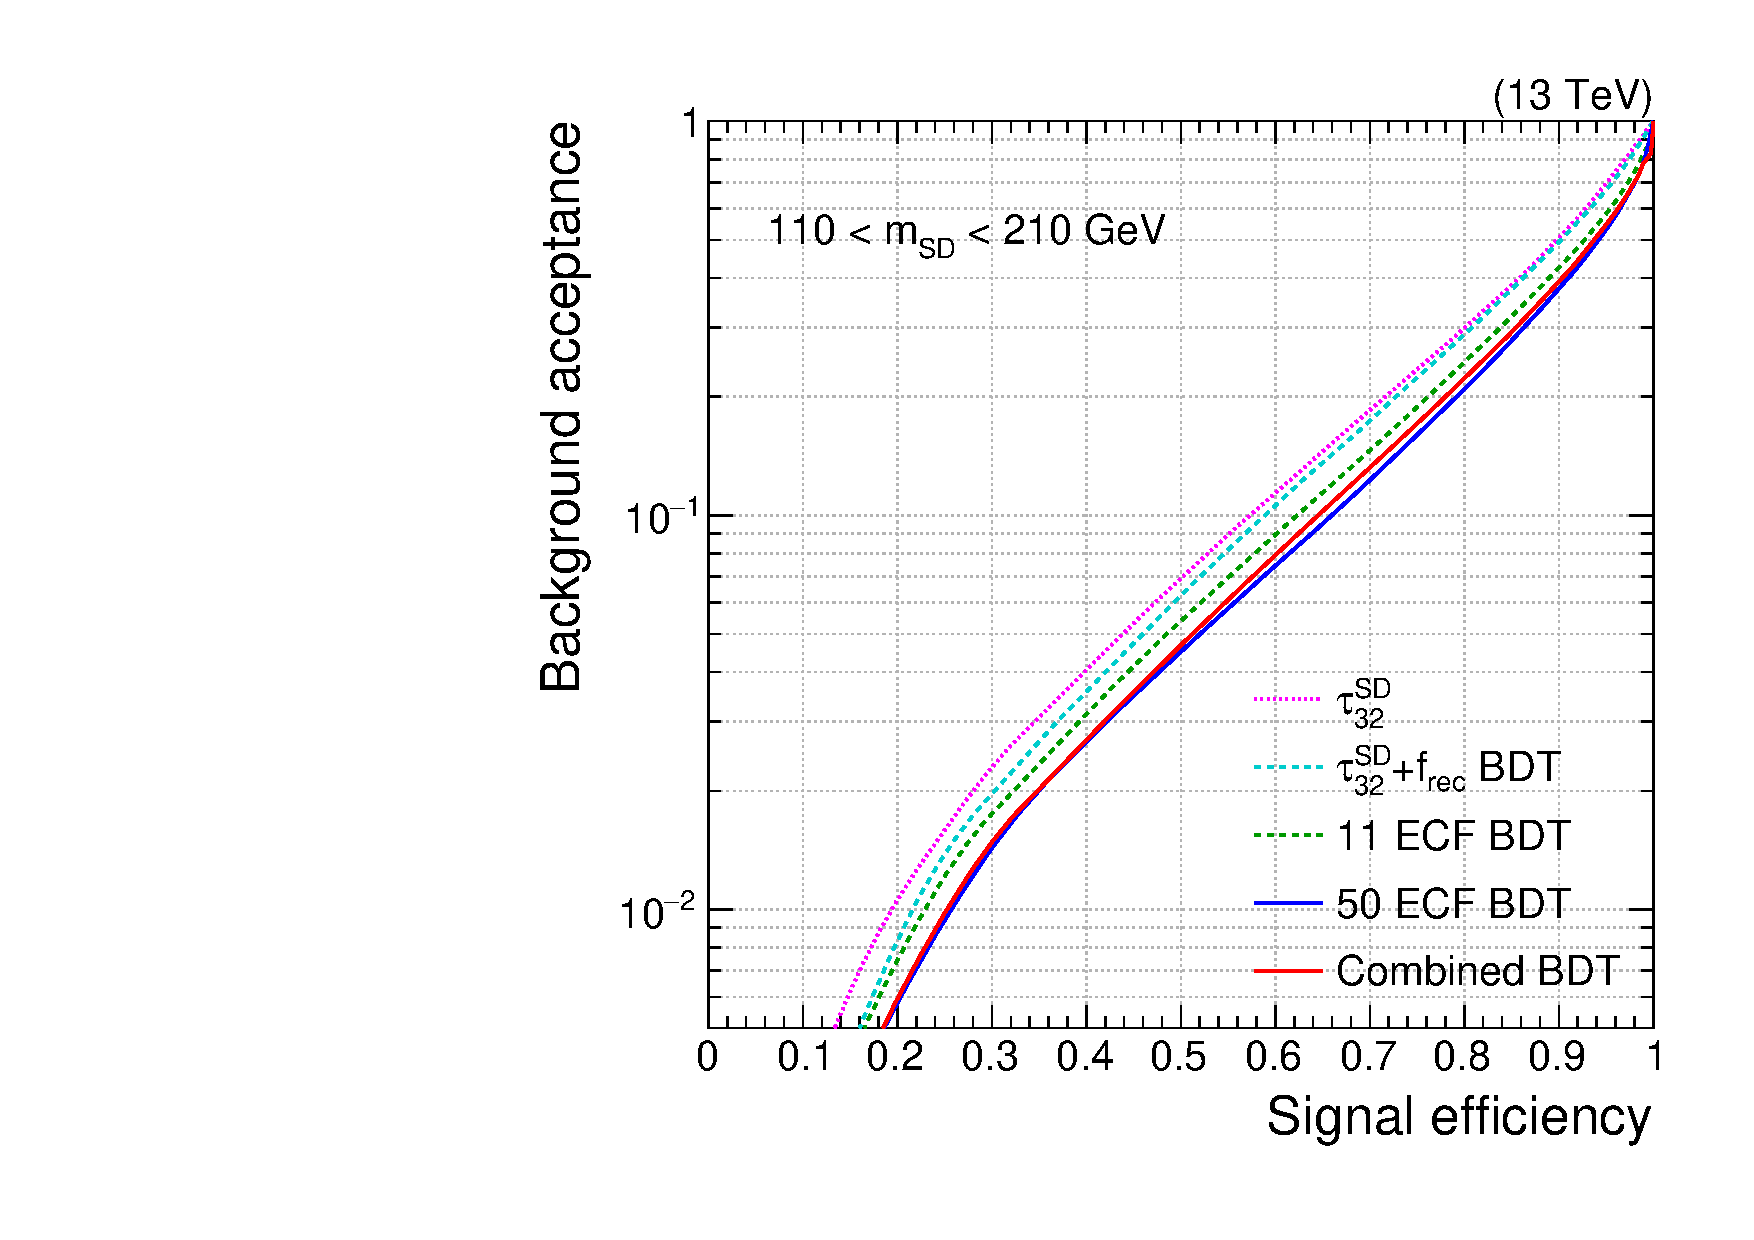
\includegraphics[width=0.5\textwidth]{figures/toptagging/bdt/roc.pdf}
        \caption{Receiver Operating Characteristic (ROC) curve comparing various top identification methods. The Combined BDT is the ID method chosen as the final tagger.}
        \label{fig:jets:roc}
    \end{center}
\end{figure}

\section{Data validation}
\label{sec:jets:sf}

Prior to using the top BDT to identify top jets and reject LQG jets, we must verify that the simulation describes the BDT distribution properly as compared to data, and correct for any residual discrepancies.
Figure~\ref{fig:jets:bdtdist} shows the BDT response and $m_\SD$ in top- and LQG-enriched selections.
Top quarks are isolated by selecting events that produce $t\bar{t}$ pairs, in which one top quark decays hadronically (the top jet) and the other decays muonically ($t\rightarrow b\mu^+\nu_mu$).
The leptonic $t$ is selected by identifying the muon and $b$ jet. 
We further require that the CA15 jet have $110<m_\SD<210$ GeV and at least one SD subjet to be $b$-tagged.
LQG jets are selected by using $Z(\rightarrow\mu\mu)$+jet events.
We require two opposite sign muons, with $|m_{\mu\mu}-m_Z|<30$ GeV; this selection selects a $\gtrsim95\%$ pure $Z$+jet sample. 
In both samples, we observe reasonably good agreement between data and simulation.

\begin{figure}[]
    \begin{center}
        \begin{subfigure}[t]{0.49\textwidth}
    \begin{center}
            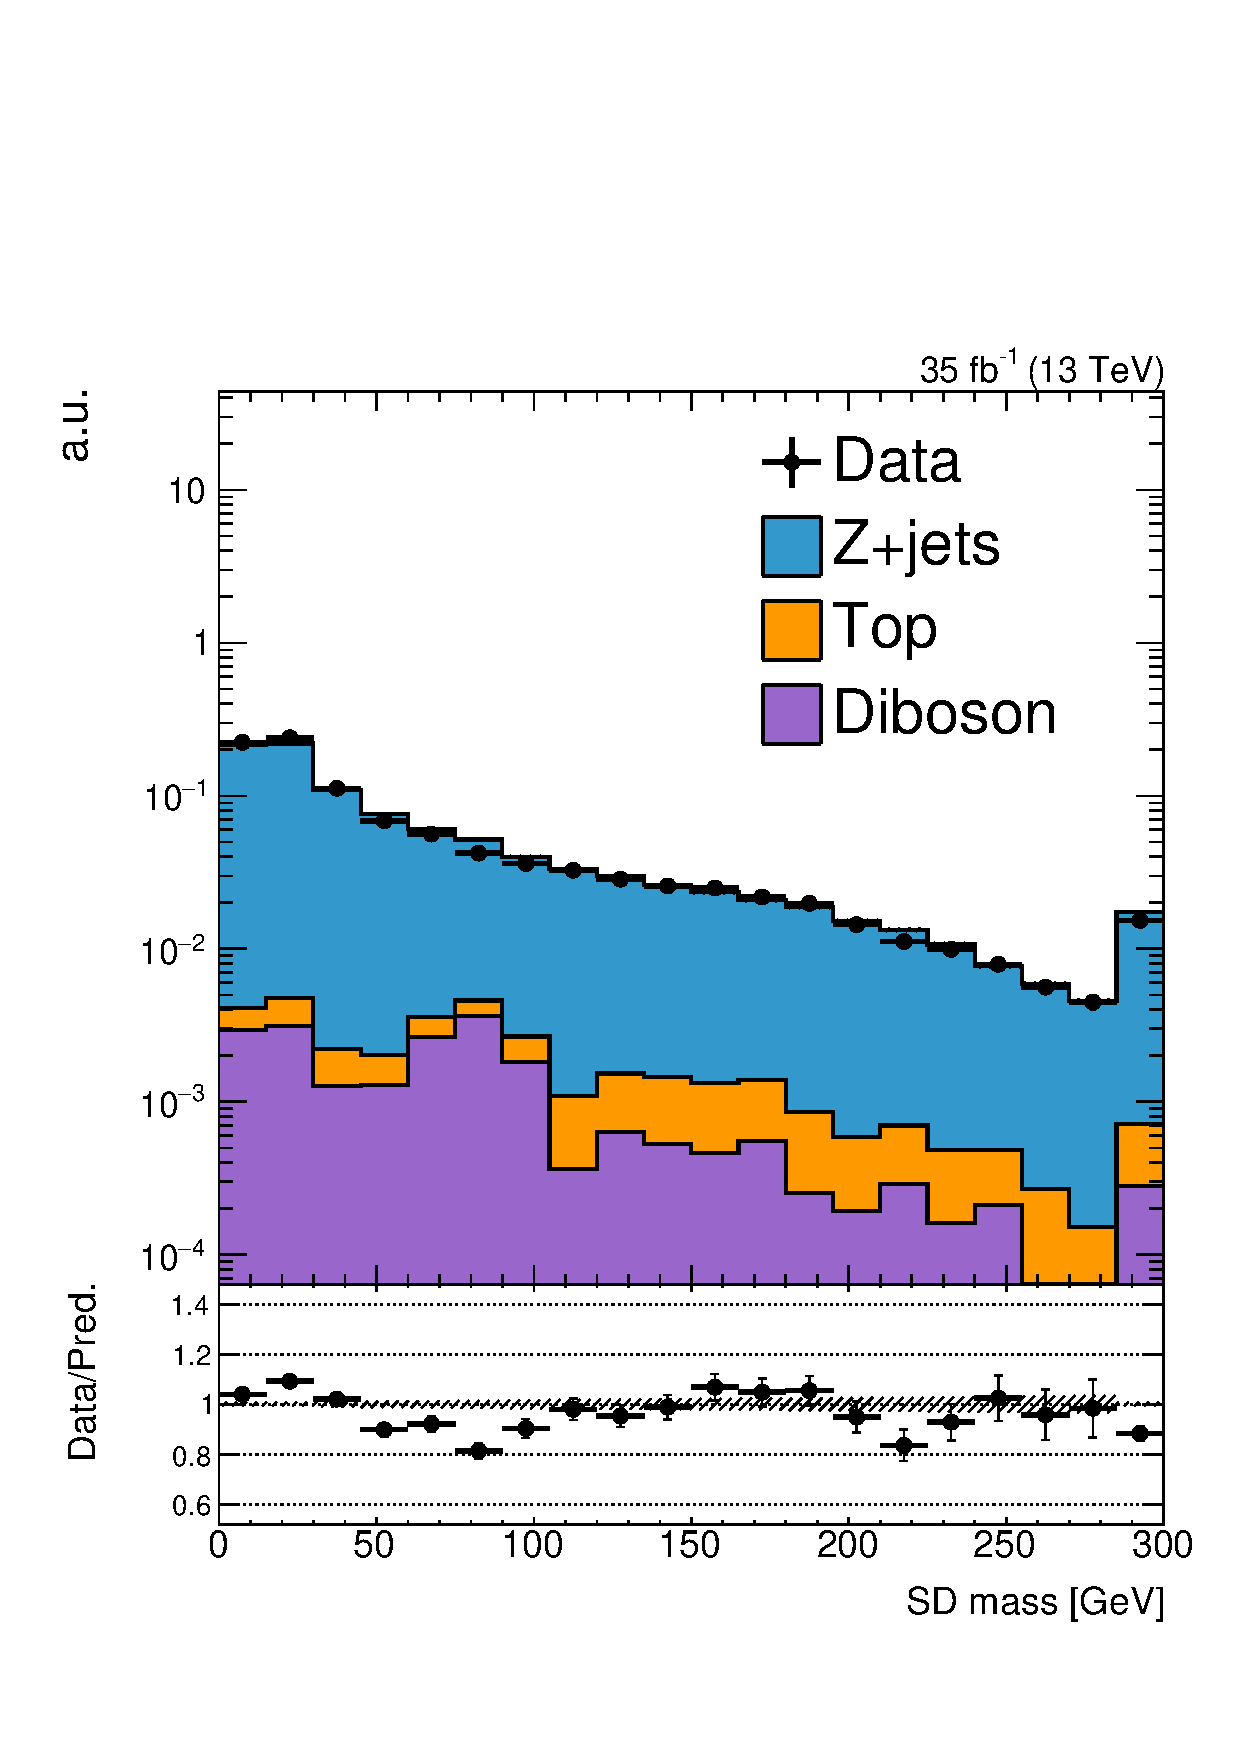
\includegraphics[width=0.49\textwidth]{figures/toptagging/sf/dimuon_fjMSD_logy.pdf}
            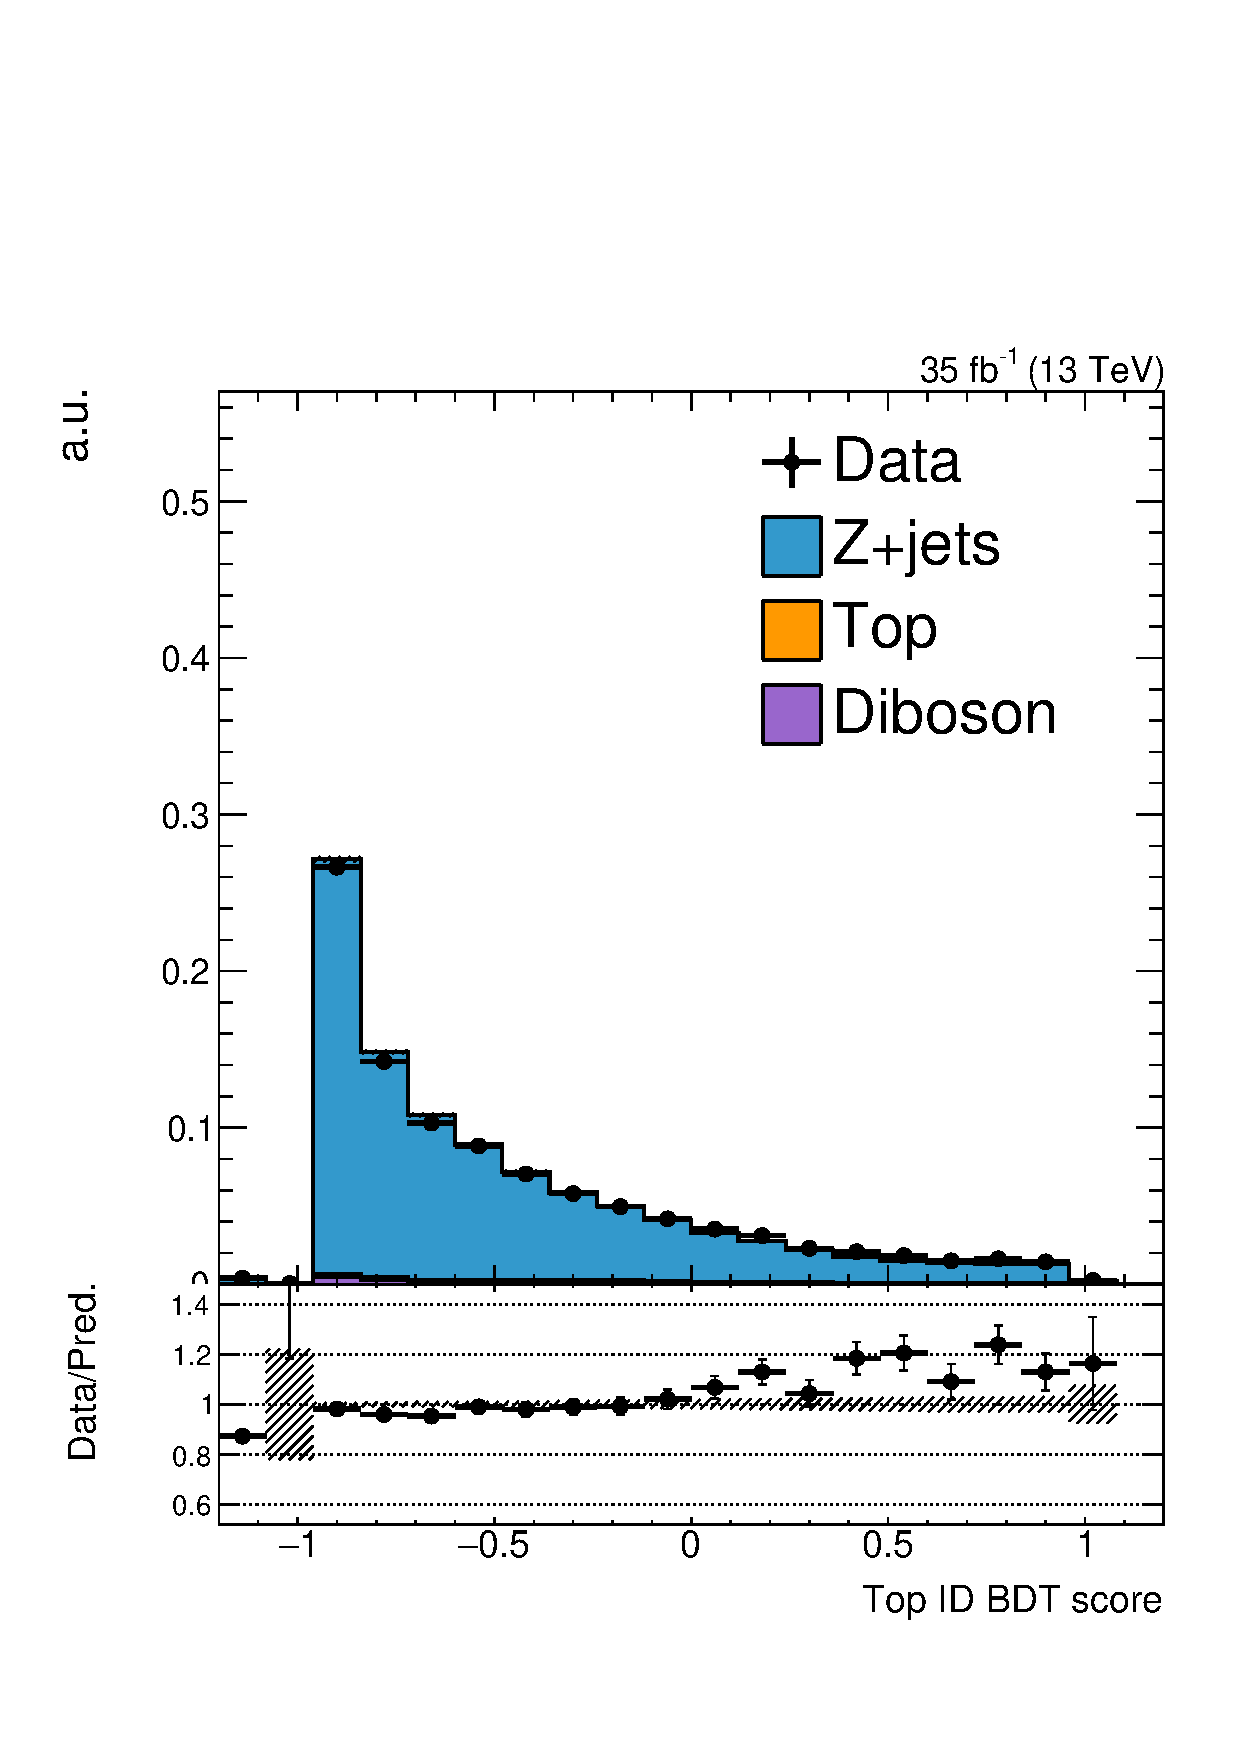
\includegraphics[width=0.49\textwidth]{figures/toptagging/sf/dimuon_top_ecf_bdt.pdf}
            \caption{Dimuon selection}
            \label{fig:jets:bdtdistmuon}
    \end{center}
    \end{subfigure} 
    \begin{subfigure}[t]{0.49\textwidth}
    \begin{center}
            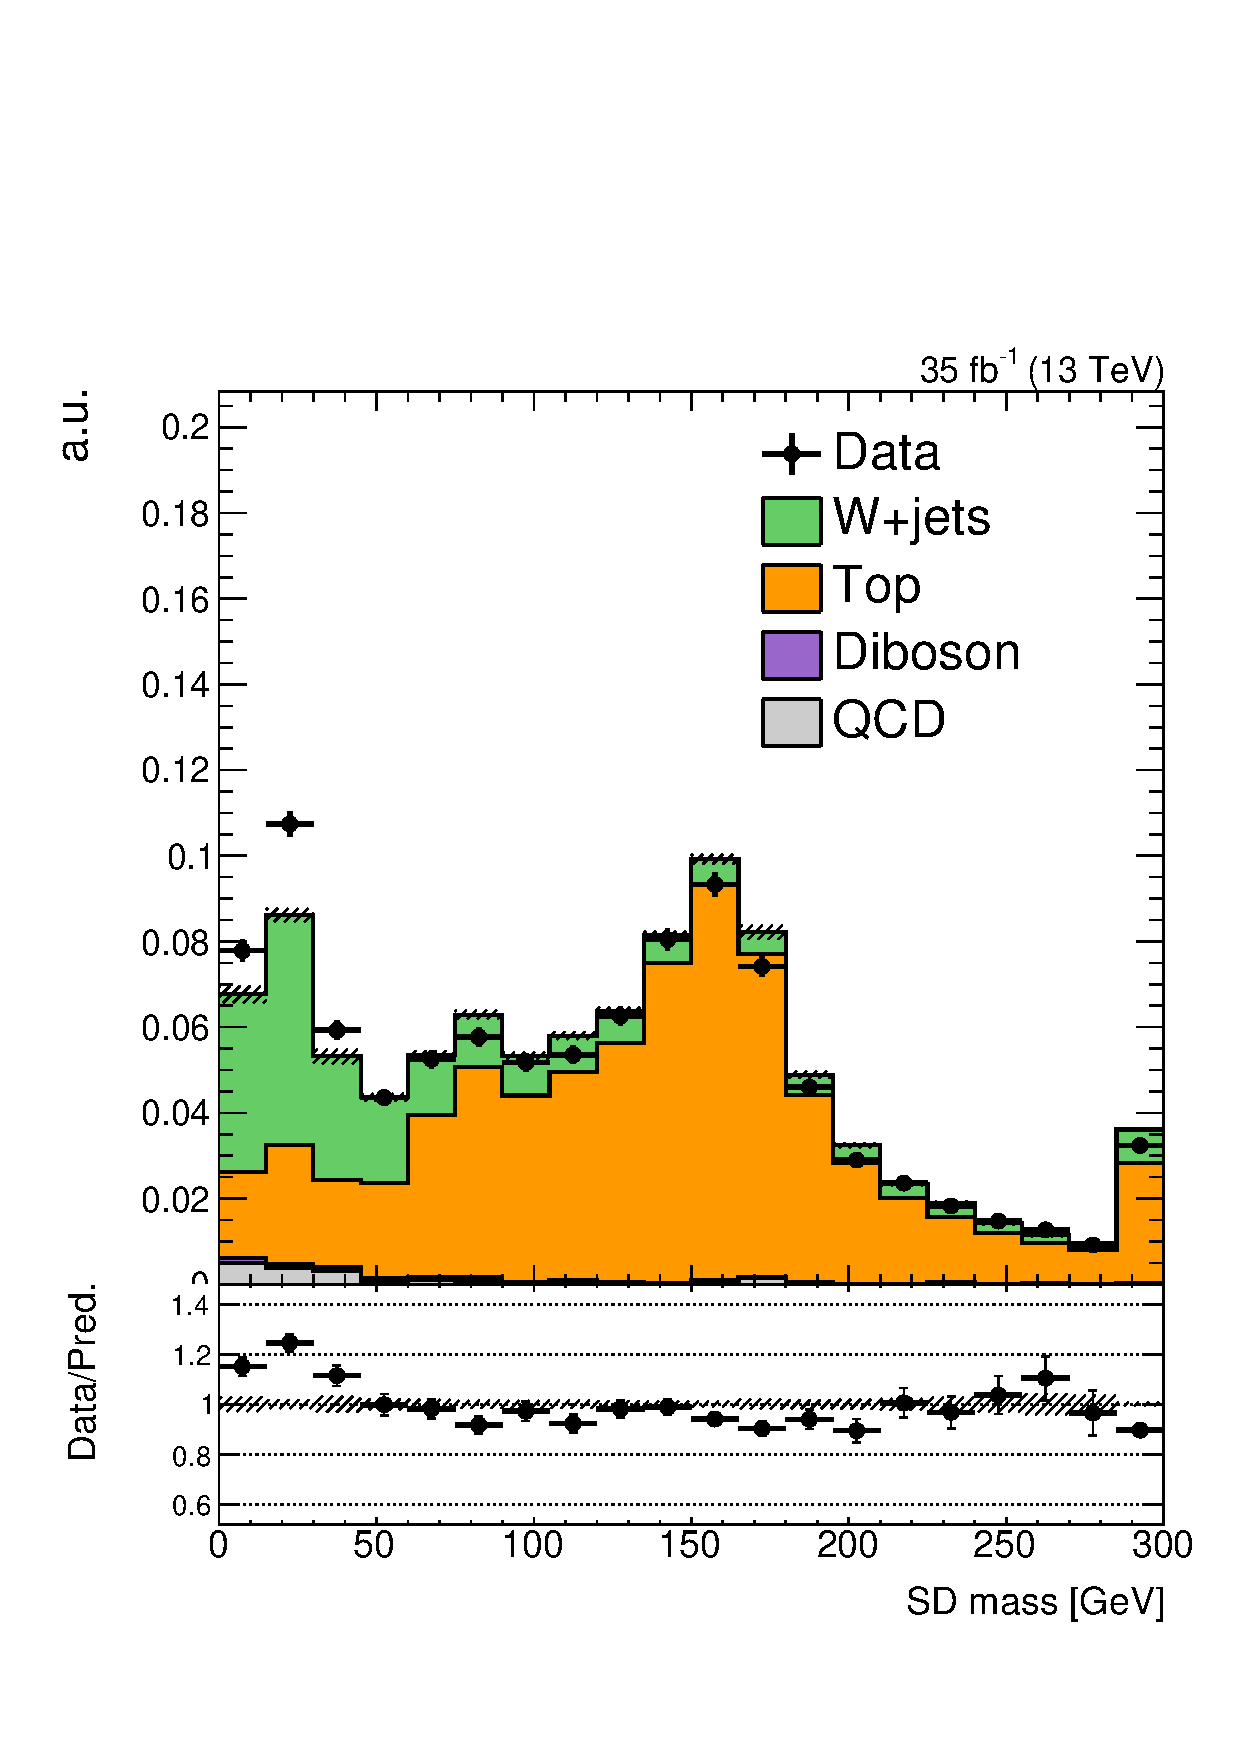
\includegraphics[width=0.49\textwidth]{figures/toptagging/sf/singlemuontop_fjMSD.pdf}
            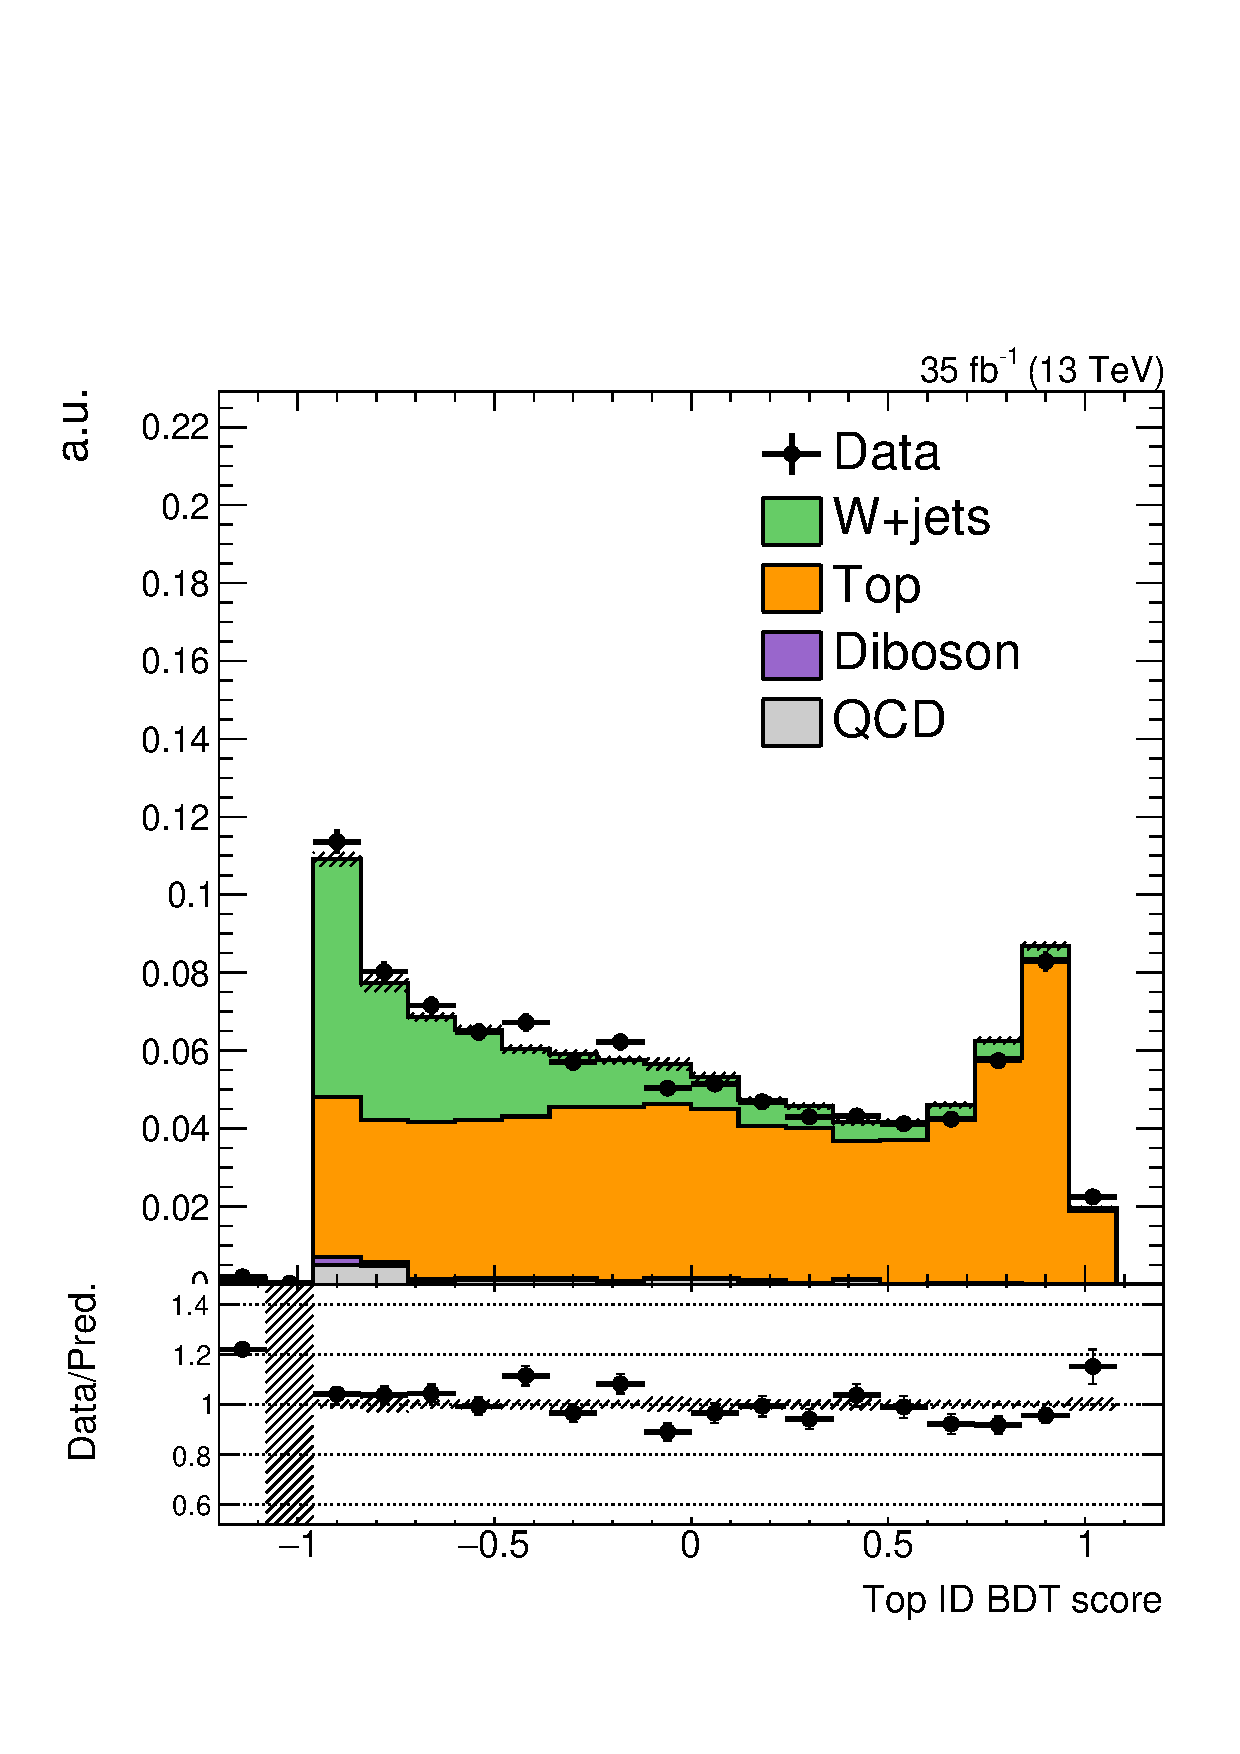
\includegraphics[width=0.49\textwidth]{figures/toptagging/sf/singlemuontop_top_ecf_bdt.pdf}
            \caption{$t\bar{t}$ selection}
    \end{center}
        \end{subfigure}
        \caption{Comparison of the BDT response and jet mass in data and simulation, in top and LQG jets.}
        \label{fig:jets:bdtdist}
    \end{center}
\end{figure}

To account for any remaining differences, we define a scale factor:
\begin{equation}
    \mathrm{SF}(x) = \frac{\epsilon_\mathrm{Data}(\mathrm{BDT}>x \text{ and }110<m_\SD<210)}{\epsilon_\mathrm{MC}(\mathrm{BDT}>x \text{ and }110<m_\SD<210)}
\end{equation}
where $x$ is a particular decision boundary and $\epsilon$ is the fraction of data or MC events passing this BDT  and mass selection.
These are chosen to optimize sensitivity to the mono-top analysis, as described in Chapter~\ref{sec:mt}.
The SF is strongly dependent on the type of jet; in particular, we expect different SFs for top and LQG jets.
In what follows, we will define two decision boundaries: loose ($x>0.1$) and tight ($x>0.45$) categories.

To compute $\mathrm{SF}_\mathrm{LQG}$, we use the dimuon selection in Figure~\ref{fig:jets:bdtdistmuon}, as this contains an essentially pure selection of LQG jets.
Two sources of uncertainty are considered: the statistical uncertainties present in the data and MC, and the uncertainties on the theoretical prediction of the cross section of the small non-LQG backgrounds ($t\bar{t}$ and diboson events).
The measured SFs are:
\begin{align}
    \mathrm{SF}_\mathrm{LQG}(0.1) = 1.02 & \pm 0.05 (\mathrm{total}) \nonumber \\ 
                                         & \pm 0.04 (\mathrm{statistical}) \pm 0.03 (t\bar{t}+\mathrm{diboson}) \nonumber \\ 
    \mathrm{SF}_\mathrm{LQG}(0.45) = 0.97 & \pm 0.07 (\mathrm{total}) \nonumber \\ 
                                         & \pm 0.06 (\mathrm{statistical}) \pm 0.03 (t\bar{t}+\mathrm{diboson})
\end{align}

The process for top jets is complicated by the fact that the top pair selection in Figure~\ref{fig:jets:bdtdist} is not sufficiently pure in merged top jets.
There is significant contamination from $W$+jets events.
Furthermore, we cannot ensure that every $t\bar{t}$ event selected produces a \emph{merged} top jet - some events may contain jets in which only part of the top's decay products are clustered into the CA15 jet.
Therefore, we extract the efficiency by means of a template fit to the mass distribution of passing and failing events, which can separate the top and LQG components in the selection.
It is for this reason that we only use groomed observables in the BDT: grooming prevents a strong correlation between the observables and $m_\SD$.
Such a correlation would cause the mass distribution of passing LQG jets to be indistinguishable from that of passing top jets.
Figure~\ref{fig:jets:sffits} show the fits in the passing and failing regions for both decision boundaries.

\begin{figure}[]
    \begin{center}
        \begin{subfigure}[t]{\textwidth}
    \begin{center}
            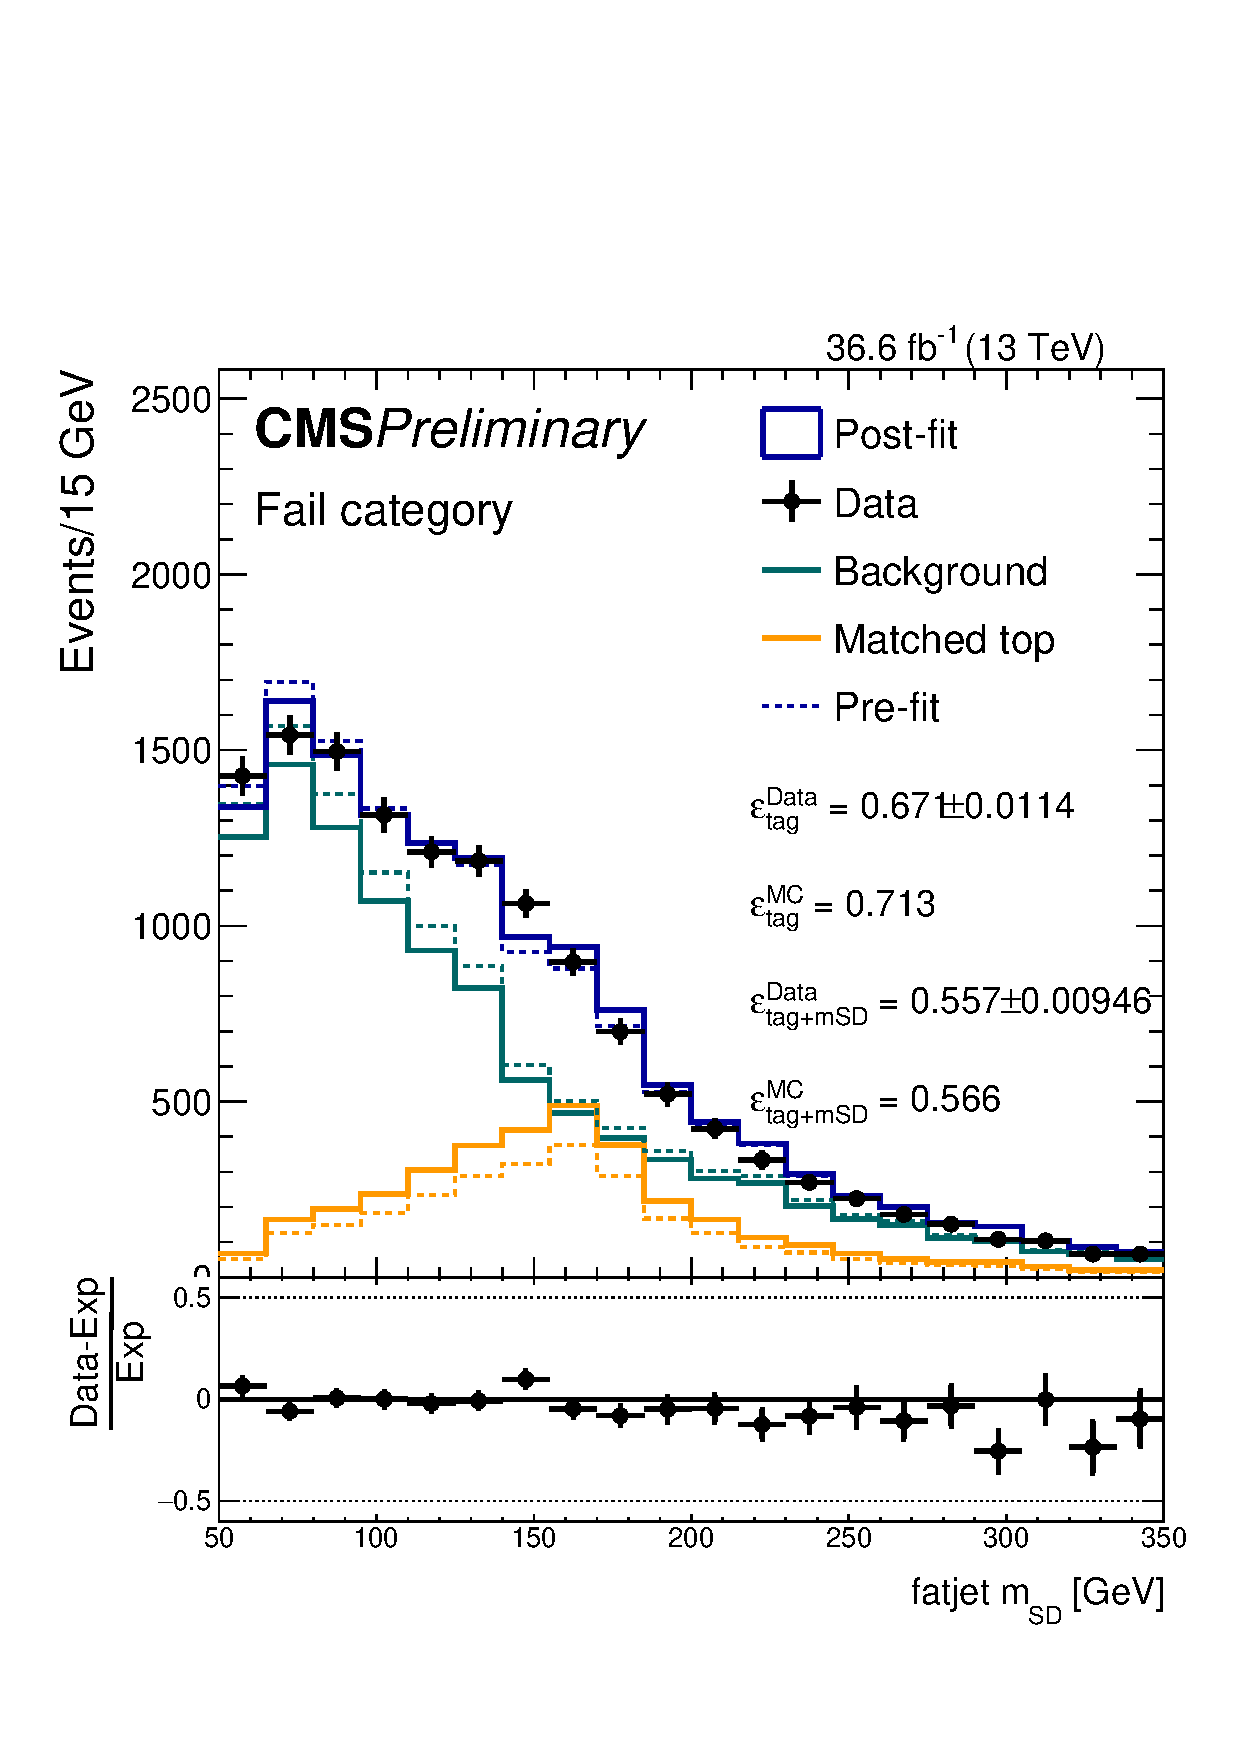
\includegraphics[width=0.35\textwidth]{figures/toptagging/sf/loose_fail.pdf}
            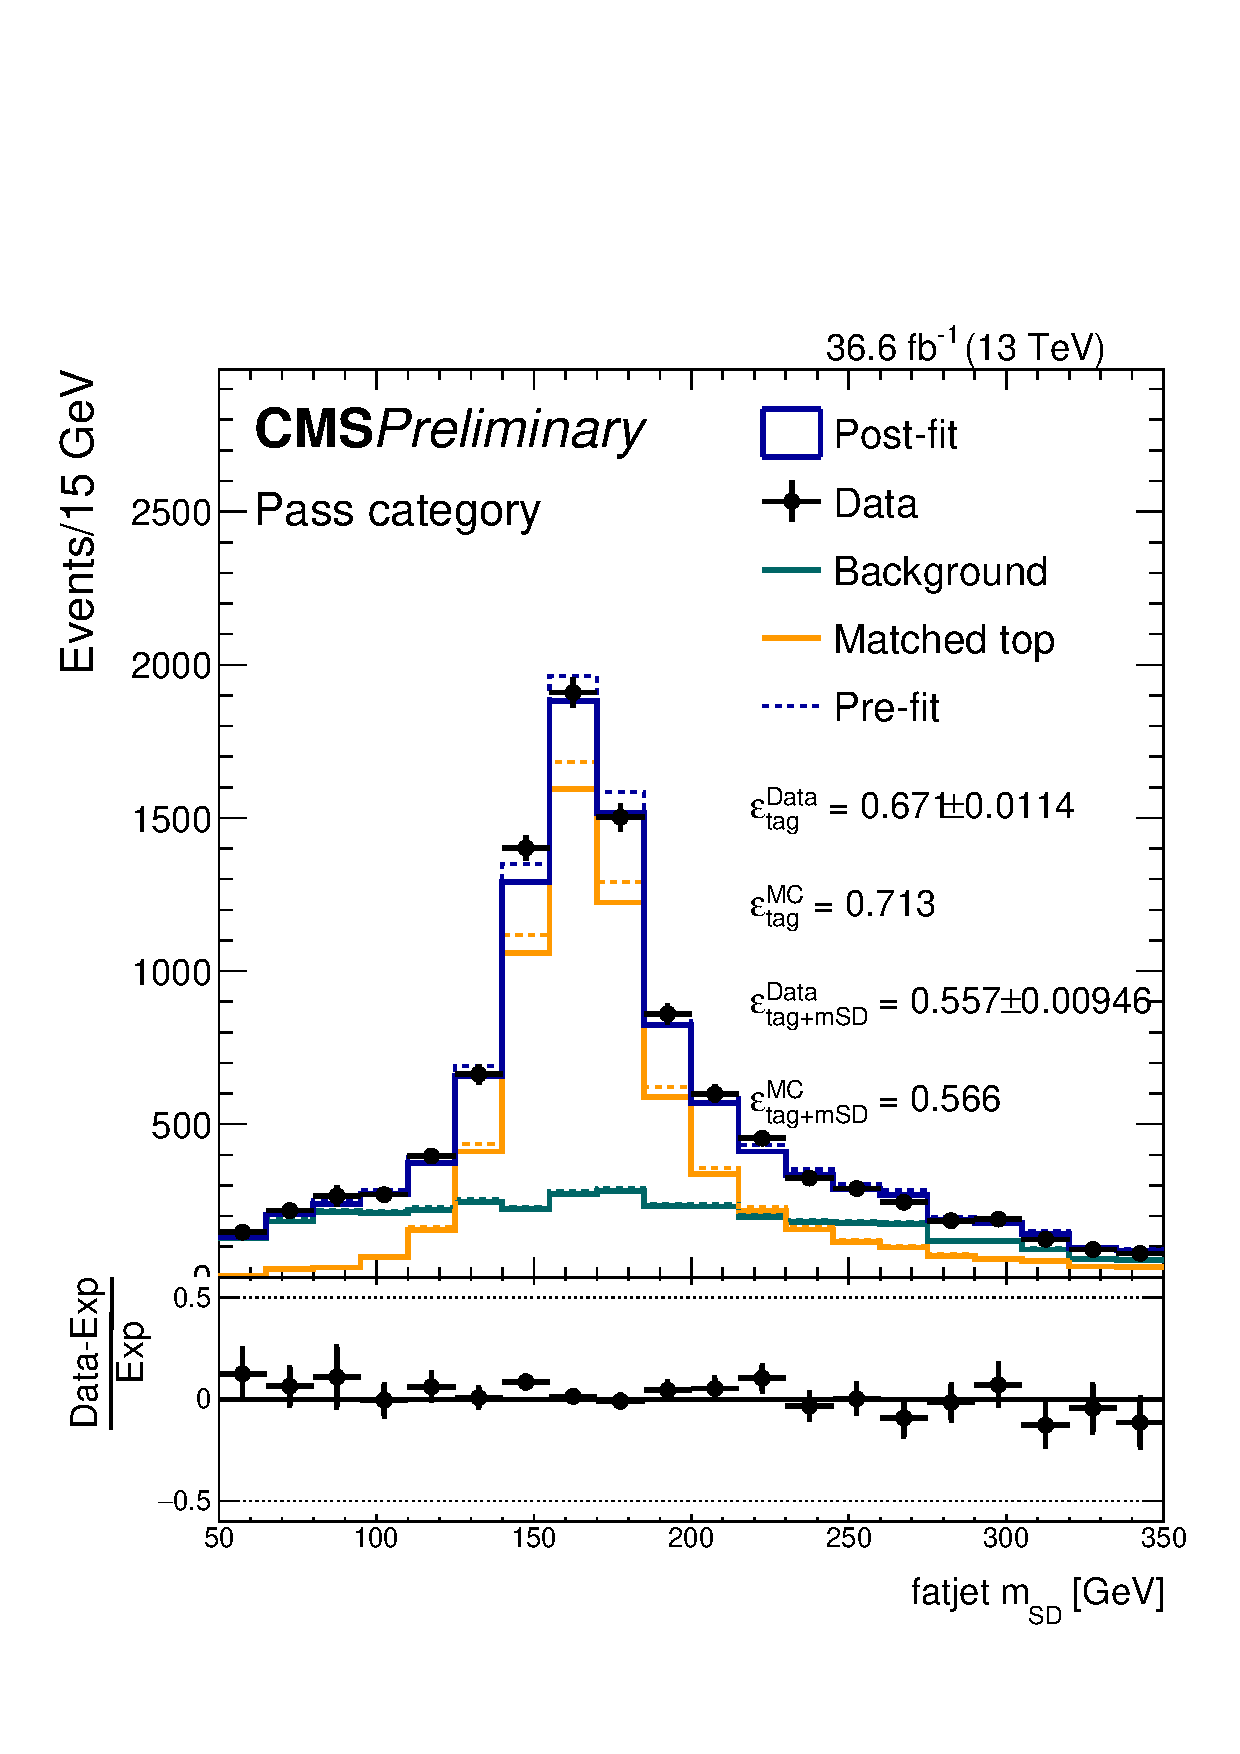
\includegraphics[width=0.35\textwidth]{figures/toptagging/sf/loose_pass.pdf}
            \caption{Loose BDT-tagged}
    \end{center}
        \end{subfigure}
        \begin{subfigure}[t]{\textwidth}
    \begin{center}
            \includegraphics[width=0.35\textwidth]{figures/toptagging/sf/tight_fail.pdf}
            \includegraphics[width=0.35\textwidth]{figures/toptagging/sf/tight_pass.pdf}
            \caption{Tight BDT-tagged}
    \end{center}
        \end{subfigure}
        \caption{Fits to the $m_\SD$ distribution in a $t\bar{t}$ sample to extract the efficiency in data of the BDT and mass selections.
                 All uncertainties plotted and quoted are statistical in nature.}
        \label{fig:jets:sffits}
    \end{center}
\end{figure}

Several sources of uncertainty are considered for this measurement:
\begin{itemize}
    \setlength\itemsep{1pt}
    \item Poisson uncertainties in the data and simulation 
    \item CA15 jet energy scale
    \item Definition used to select \emph{merged top} jets, allowing $\max \Delta R_{qq'}$ to vary between 1 and 1.5 (nominal value is 1.2)
    \item Efficiency of selecting $b$ jets
\end{itemize}
The resultant SFs and associated uncertainties are:
\begin{align}
    \mathrm{SF}_\mathrm{top}(0.1) = 1.08 & \pm 0.04 (\mathrm{total}) \nonumber \\ 
                                         & \pm 0.03 (\mathrm{statistical}) \pm 0.02 (\mathrm{JES+JER}) \pm 0.02 (\mathrm{merging}) \pm 0.002 (b) \nonumber \\ 
    \mathrm{SF}_\mathrm{top}(0.45) = 1.07 & \pm 0.06 (\mathrm{total}) \nonumber \\ 
                                         & \pm 0.03 (\mathrm{statistical}) \pm 0.02 (\mathrm{JES+JER}) \pm 0.014 (\mathrm{merging}) \pm 0.000 (b) 
\end{align}

